\phantomsection
\chapter[Classifying White Blood Cells]{Classifying White Blood Cells}
\label{chapter:white_blood_cells}
\renewcommand{\chaptertitle}{Classifying White Blood Cells}
\addcontentsline{cc}{chapter}{Chapter \thechapter} % Adds chapter number to table of contents

%\clearpage \null
%\thispagestyle{empty}
%\AddToShipoutPictureBG*{% Add picture to current page
%  \AtStockLowerLeft{% Add picture to lower-left corner of paper stock
%    \includegraphics[width=\stockwidth]{images/CMYK_ed3/cover/alignment_final}}
%}
%\addtocounter{page}{-1}
%\clearpage

\FloatBarrier

\section{Introduction: How Are Blood Cells Counted?}
\label{sec:introduction}
\phantomsection

Your doctor sometimes counts your blood cells to ensure that they are within healthy ranges as part of a complete blood count. These cells comprise \textdef{red blood cells (RBCs)}{red blood cells (RBCs)}{cells in blood that transport oxygen via the hemoglobin protein}, which transport oxygen via the hemoglobin protein, and \textdef{white blood cells (WBCs)}{white blood cells (WBCs)}{cells that help identify and attack foreign cells as part of the immune system}, which help identify and attack foreign cells as part of your immune system.

The classic device used for counting blood cells is the \textdefnogloss{hemocytometer}. In this device, a technician filters a small amount of blood onto a gridded slide (\autoref{fig:hemocytometer}) and then counts the number of cells of each type in the squares on the grid. As a result, the technician can estimate the number of each type of cell per volume of blood.\\

\begin{figure}[h]
\centering
\tabcolsep = 1em
\mySfFamily
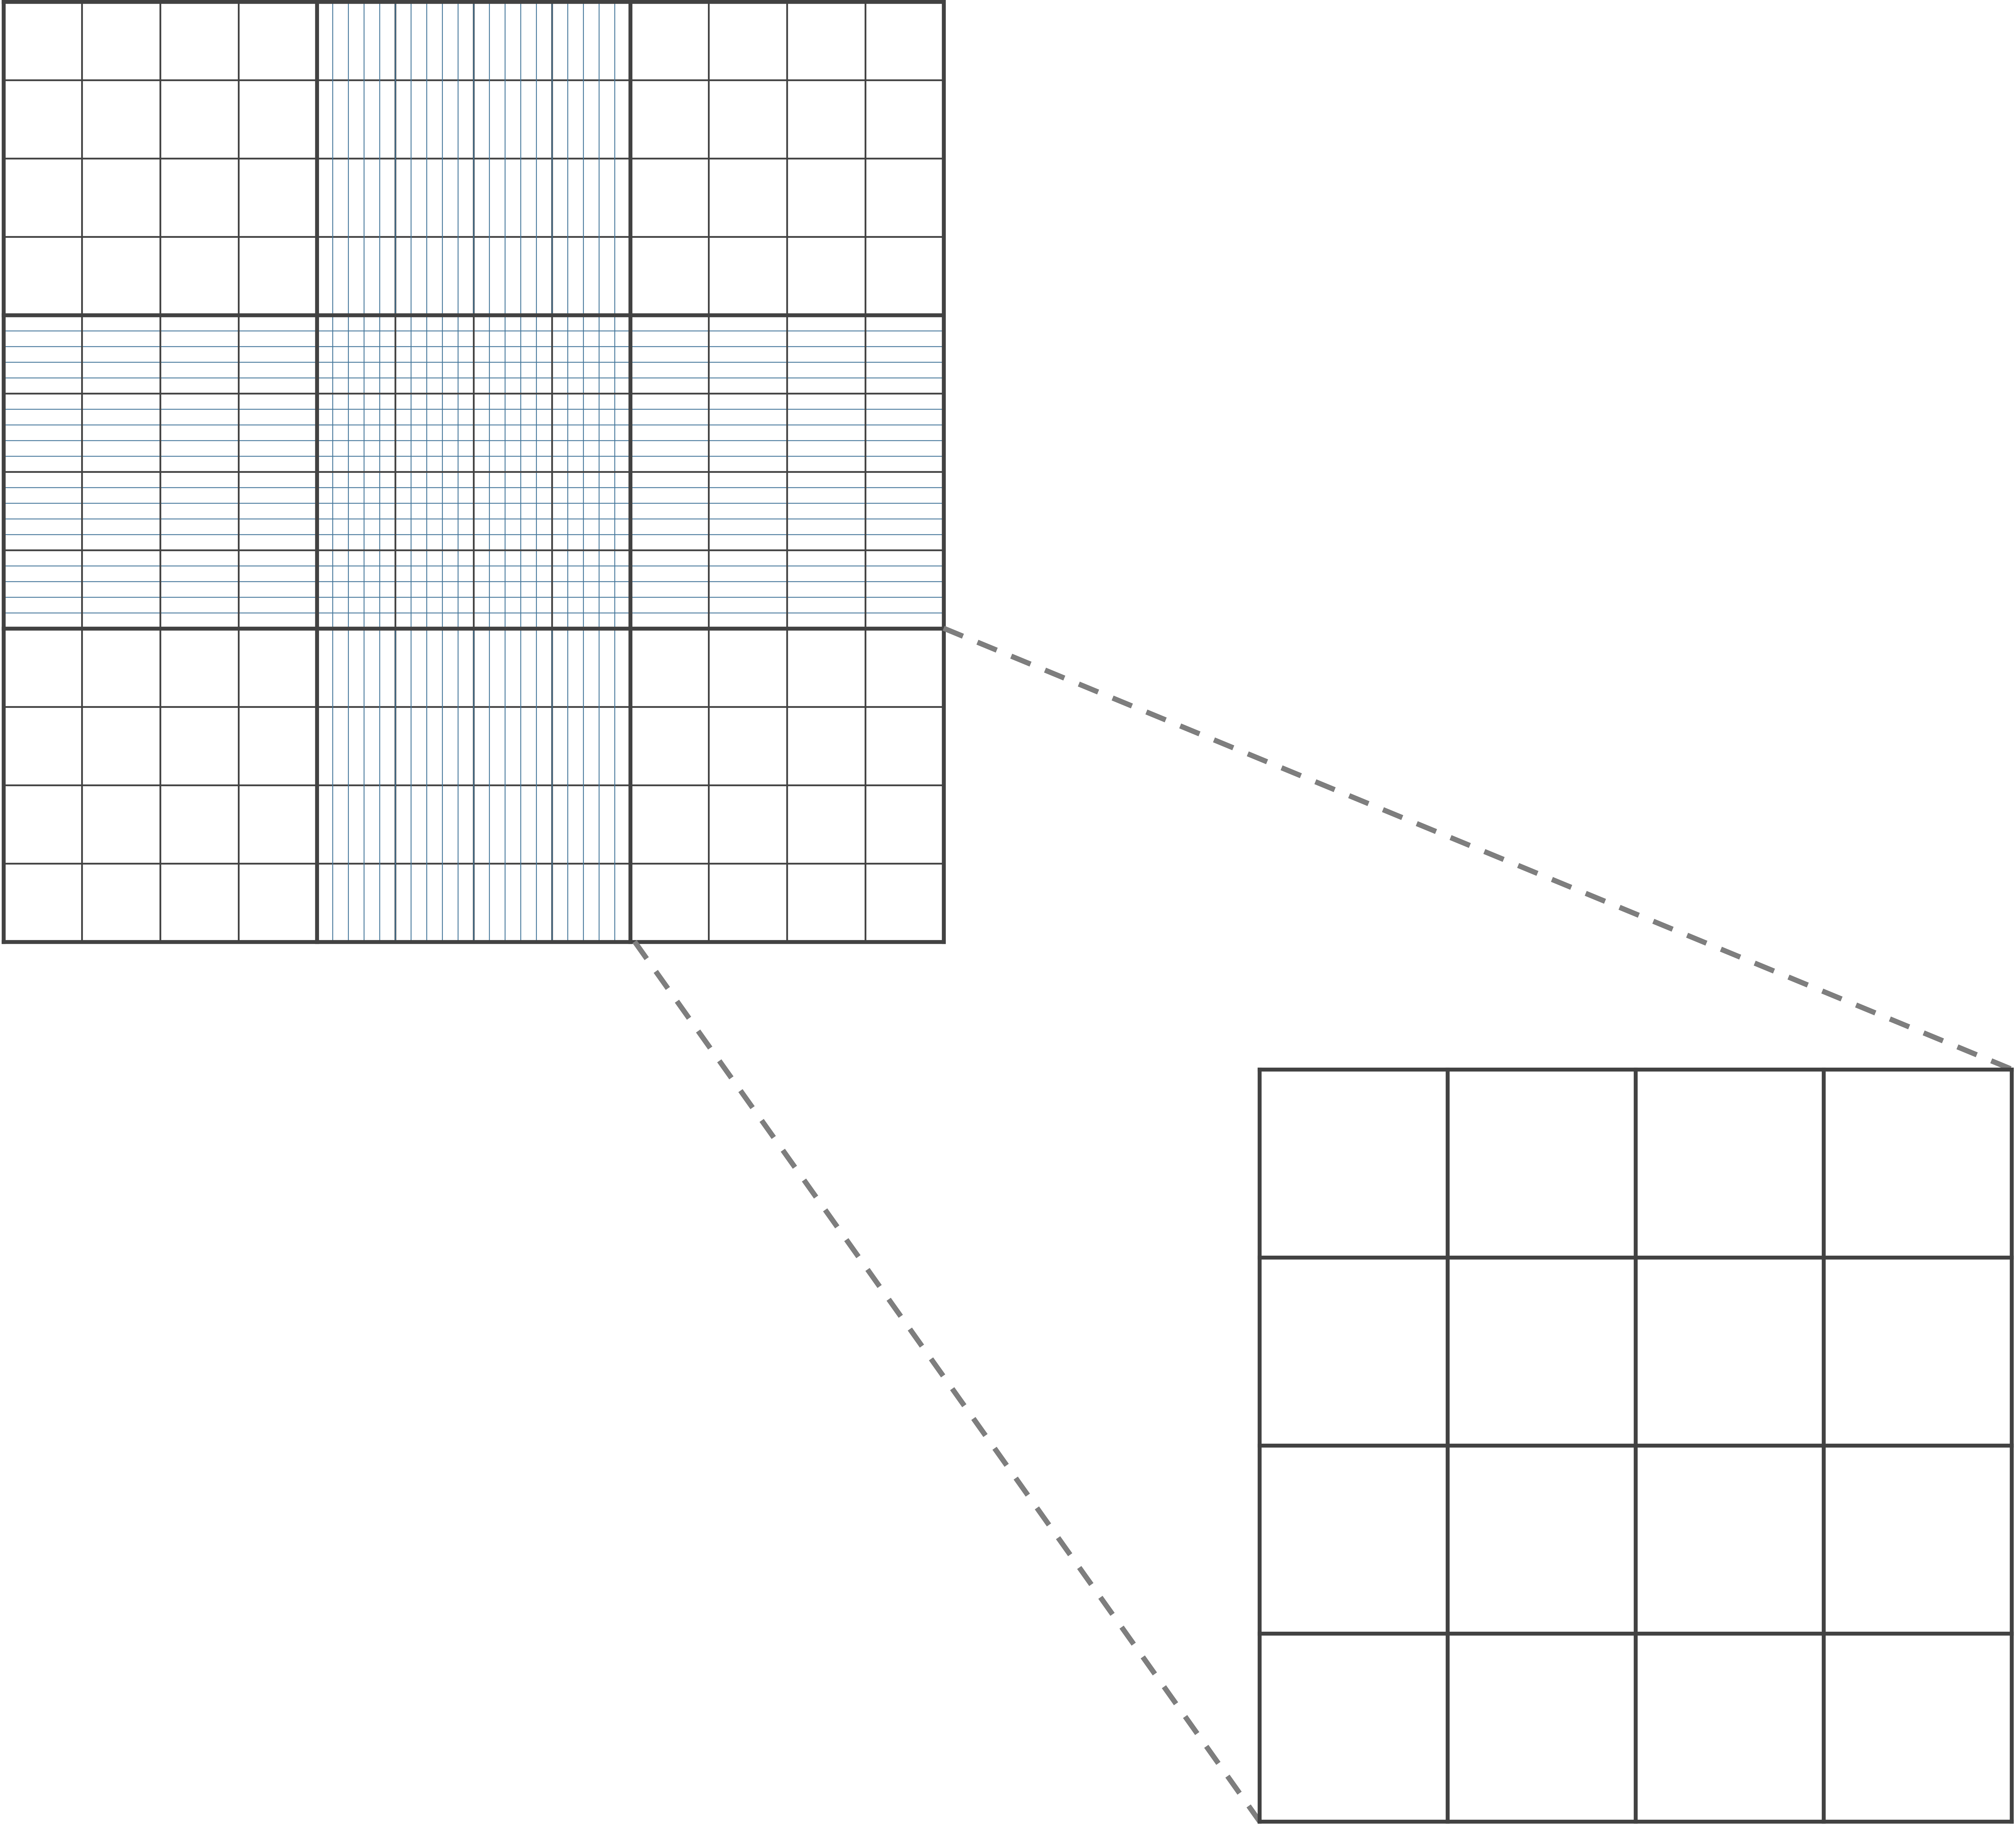
\includegraphics[width = 0.7\textwidth]{../images/hemocytometer.png}
\caption{(Left) A schematic of a 3 mm by 3 mm hemocytometer, showing grid lines with differing widths. (Right) A hypothetical blood smear within a 0.25 mm by 0.25 mm square, which contains a volume of blood equaling 0.00000625 mL. By counting the number of cells in a number of squares, researchers can estimate the counts of cells per unit volume of blood.}
\label{fig:hemocytometer}
\end{figure}

\begin{qbox}[%
How could the volume of a blood sample influence the estimate of blood cell count?
]\end{qbox}

You would not be wrong to think that the hemocytometer seems old-fashioned, as it was invented by Louis-Charles Malassez 150 years ago. To reduce the human error inherent in using this device, what if we train a computer to count blood cells for us?

We will focus our work on WBCs. WBCs divide into families based on their structure and function, with some diseases causing an abnormally low or high count of cells in a specific WBC class. In this chapter, we therefore have two aims. First, can we excise, or \textdef{segment}{segmentation}{the process of partitioning an image in order to excise objects of interest}, WBCs from cellular images?  Second, can we \textdef{classify}{classification}{the seminal problem of (correctly) categorizing a collection of data} WBCs into their appropriate types?

We will work with a publicly available dataset (\url{https://github.com/Shenggan/BCCD_Dataset}) containing blood cell images that depict both RBCs and WBCs (\autoref{fig:three_families}). The cells have been stained with a red-orange dye that bonds to hemoglobin and a blue dye that bonds to DNA and RNA. RBCs lack a nucleus and will only absorb the red-orange dye, whereas WBCs have a nucleus but lack hemoglobin and will only absorb the blue dye.

\autoref{fig:three_families} also illustrates the three main families of WBCs: \textdefnogloss{granulocytes} (left), \textdefnogloss{monocytes} (center), and \textdefnogloss{lymphocytes} (right).  Granulocytes have a \textdef{multilobular nucleus}{multilobular nucleus}{a nucleus consisting of several round ``lobes'' that are linked by thin strands of nuclear material}, which consists of several round ``lobes'' that are linked by thin strands of nuclear material. Monocyte and lymphocyte nuclei only have a single lobe, but monocyte nuclei have a more irregular shape, whereas lymphocyte nuclei are more rounded and take up a greater fraction of the cell's volume.\\

\begin{figure}[h]
\centering
\tabcolsep = 1em
\mySfFamily
\begin{tabular}{c c c}
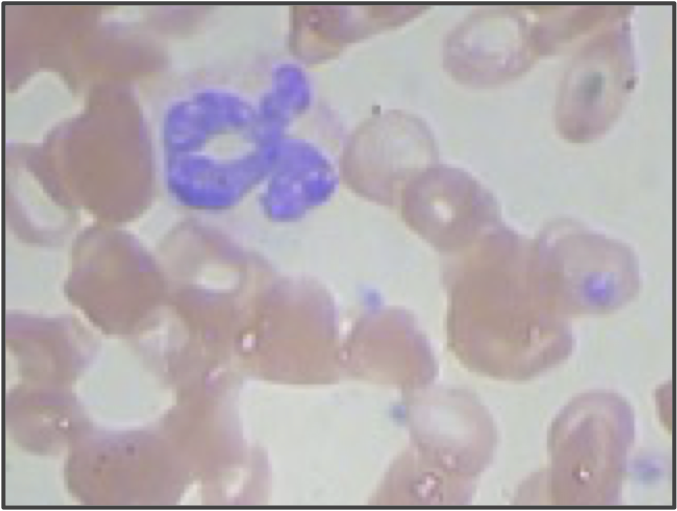
\includegraphics[width = 0.25\textwidth]{../images/neutrophil.png} & 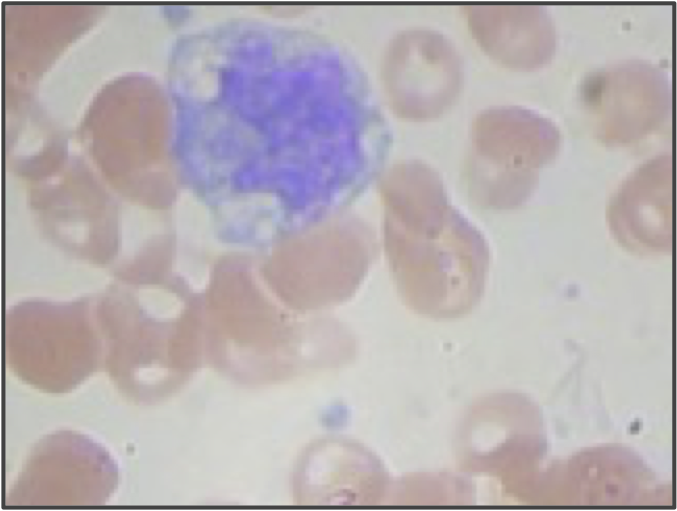
\includegraphics[width = 0.25\textwidth]{../images/monocyte.png} & 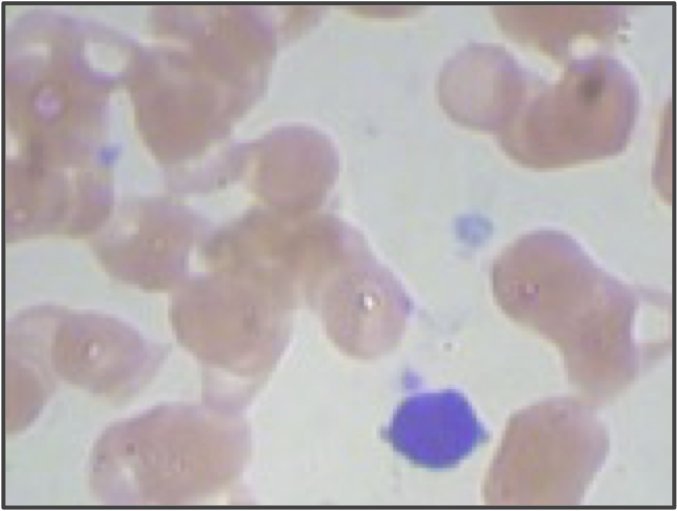
\includegraphics[width = 0.25\textwidth]{../images/lymphocyte.png}
\end{tabular}
\caption{Three images from the blood cell image dataset showing three types of WBCs. In our dataset, these cells correspond to image IDs 3, 15, and 20. (Left) A specific subtype of granulocyte called a neutrophil, illustrating the multilobular structure of this WBC family. (Center) A monocyte with a single, irregularly-shaped nucleus. (Right) A lymphocyte with a small, round nucleus.}
\label{fig:three_families}
\end{figure}

When you look at the cells in \autoref{fig:three_families}, you may think that our work will be easy. Segmenting WBCs only requires identifying the large purplish regions, and classifying them is just a matter of categorizing them according to the differences in shape that we described above. Yet even after decades of research into computer vision, researchers struggle to attain the precision of the human eye, which is the result of billions of years of evolution.\\

\FloatBarrier
\phantomsection

\section{Segmenting White Blood Cell Images}
\label{sec:segmenting_white_blood_cell_images}
\phantomsection
\subsection{Image segmentation requires a tailored approach}

We begin our work by discussing how to segment WBCs from blood cell images. Researchers have developed many algorithms for cellular image segmentation, but no single approach can be used in all contexts. We therefore will identify the key attributes that make this dataset special, which we will use to develop our own segmentation algorithm.

What makes the WBC nucleus so easy for a human to spot in the images in \autoref{fig:three_families}? You may be screaming, ``The nucleus is dark blue! How hard could it be?'' But to train a computer to segment images by color, we should first understand how the computer encodes color in images.

\FloatBarrier
\phantomsection
\subsection{The RGB color model}

In the \textdef{RGB color model}{RGB color model}{a model in which every rectangular pixel on a computer screen emits a single color formed as a mixture of red, green, and blue}, every rectangular pixel on a computer screen emits a single color formed as a mixture of differing amounts of the three primary colors of light: red, green, and blue (hence the acronym ``RGB''). The amount of each primary color in a pixel is expressed as an integer between 0 and 255, inclusively, with larger integers corresponding to greater amounts of the color.

A few colors are shown in \autoref{fig:RGB_color_chart} along with their RGB equivalents; for example, magenta corresponds to equal parts red and blue. Note that a color like (128, 0, 0) contains only red but appears duskier than (256, 0, 0) because the red light in that pixel has not been fully “turned on”.\\

\begin{figure}[h]
\centering
\mySfFamily
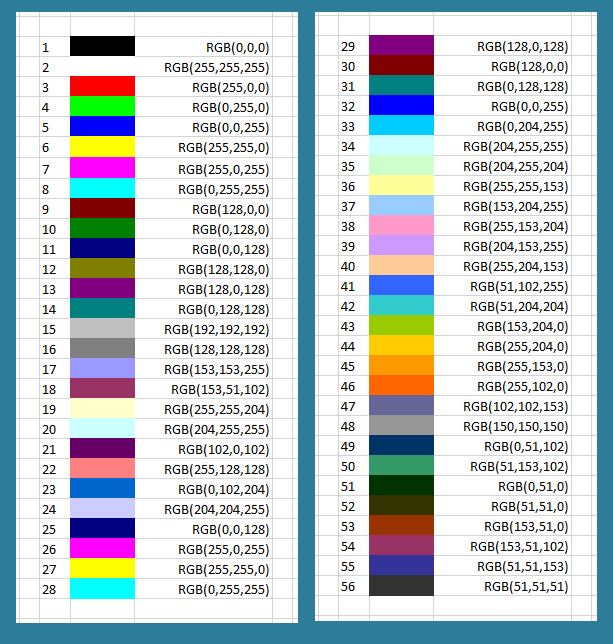
\includegraphics[width = 0.55\textwidth]{../images/RGB_color_chart.png}
\caption{A collection of colors along with their RGB codes. This table corresponds to mixing colors of light instead of pigment, which causes some non-intuitive effects; for example, yellow is formed by mixing equal parts red and green. The last six colors appear muted because they only receive half of a given color value compared to a color that receives 256 units. If all three colors are mixed in equal proportions, then we obtain a color on the gray scale between white (maximum amount of all three colors) and black (no color).}
\label{fig:RGB_color_chart}
\end{figure}

The RGB model gives us an idea for segmenting a WBC nucleus. If we scan through the pixels in a blood cell image, we can ignore any pixels whose RGB color values are not sufficiently blue; hopefully, the remaining pixels are found in the WBC nucleus.\\

\begin{qbox}[%
You can find a color picker in \texttt{Utilities > Digital Color Meter} (Mac OS X) or by using ShareX  (Windows). Open your color picker, and hover the picker over different parts of the granulocyte image in \autoref{fig:three_families} (left). What are the typical RGB values for the WBC nucleus, and how do these RGB values differ from those of the RBCs and the image background?
]\end{qbox}

\FloatBarrier
\phantomsection
\subsection{Binarizing an image based on a color threshold}

We will \textdefnogloss{binarize} each blood cell image by coloring a pixel white (RGB: (256, 256, 256)) if its blue value is above some threshold, and turning a pixel black (RGB: (0, 0, 0)) if its blue value is beneath some threshold. The binarized version of the granulocyte image from \autoref{fig:three_families} (left) using the threshold value of 153 is shown in \autoref{fig:neutrophil_binarized_blue}. Unfortunately, we cannot clearly see the WBC nucleus in this binarized image because although the nucleus's pixels have high blue values, so do those of the image's background, which emit high percentages of red, green, and blue, producing the background's light appearance.\\

\begin{figure}[h]
\centering
\mySfFamily
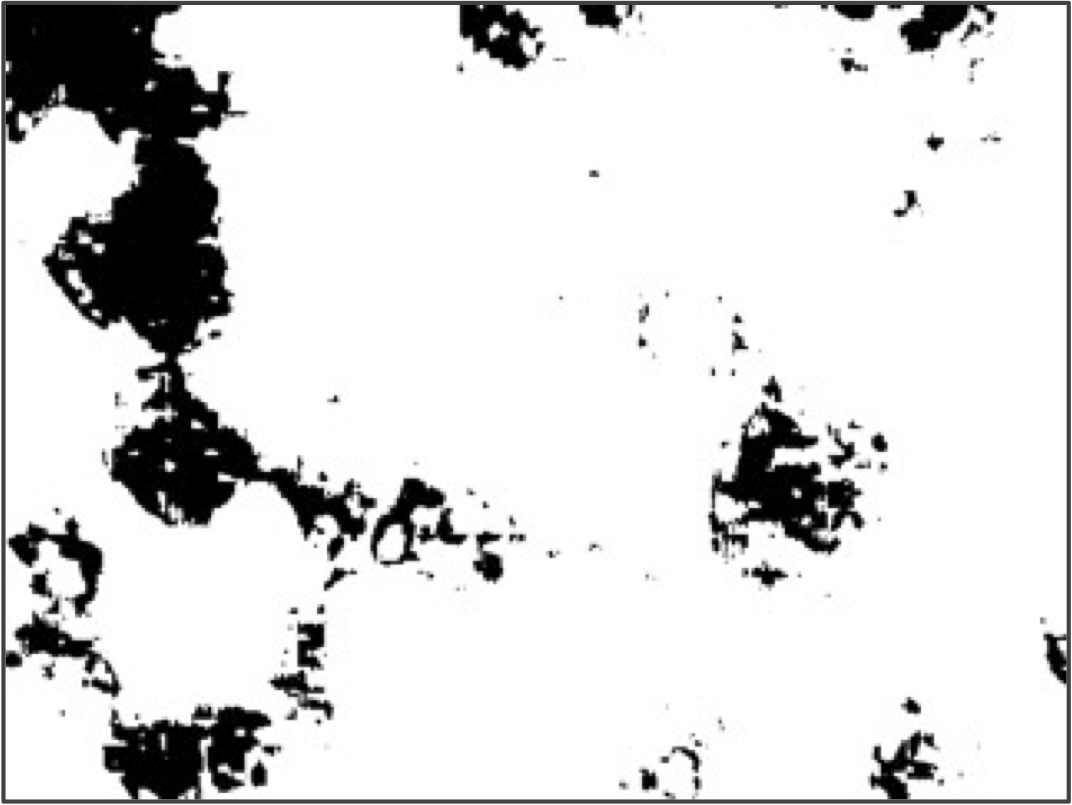
\includegraphics[width = 0.4\textwidth]{../images/neutrophil_binarized_blue.png}
\caption{A binarized version of the granulocyte image from \autoref{fig:three_families} (left). A pixel is colored white if it has a blue value of 153 or greater, and a pixel is colored black otherwise. The region with the nucleus is not clearly visible because much of the original image's background is light, and so its pixels have large red, green, and blue values.}
\label{fig:neutrophil_binarized_blue}
\end{figure}

\begin{qbox}[%
How might we modify our segmentation approach to perform a binarization that identifies the WBC nucleus more effectively?
]\end{qbox}

We were unable to distinguish between the image background and the WBC nucleus using blue color values, but a color picker verifies that pixels in the WBC nucleus tend to have a green value that is much lower than the image background and a red value that is lower than every other part of the image. \autoref{fig:neutrophil_binarized_other_colors} shows two binarizations of the original image using a green threshold of 153 (left) and a red threshold of 166 (right).

\begin{figure}[h]
\centering
 \tabcolsep = 1em
\mySfFamily
\begin{tabular}{c c}
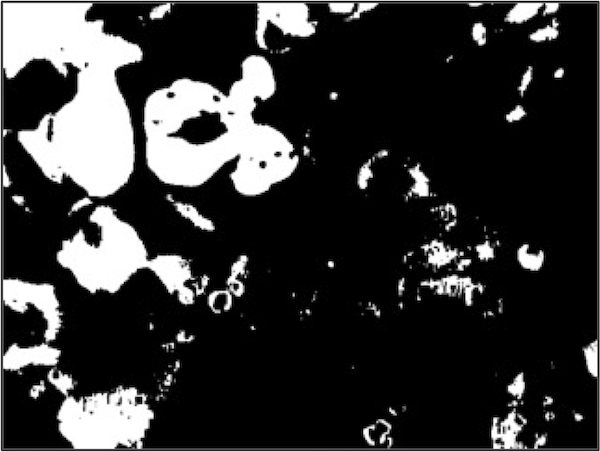
\includegraphics[width = 0.4\textwidth]{../images/neutrophil_binarized_green.png} & 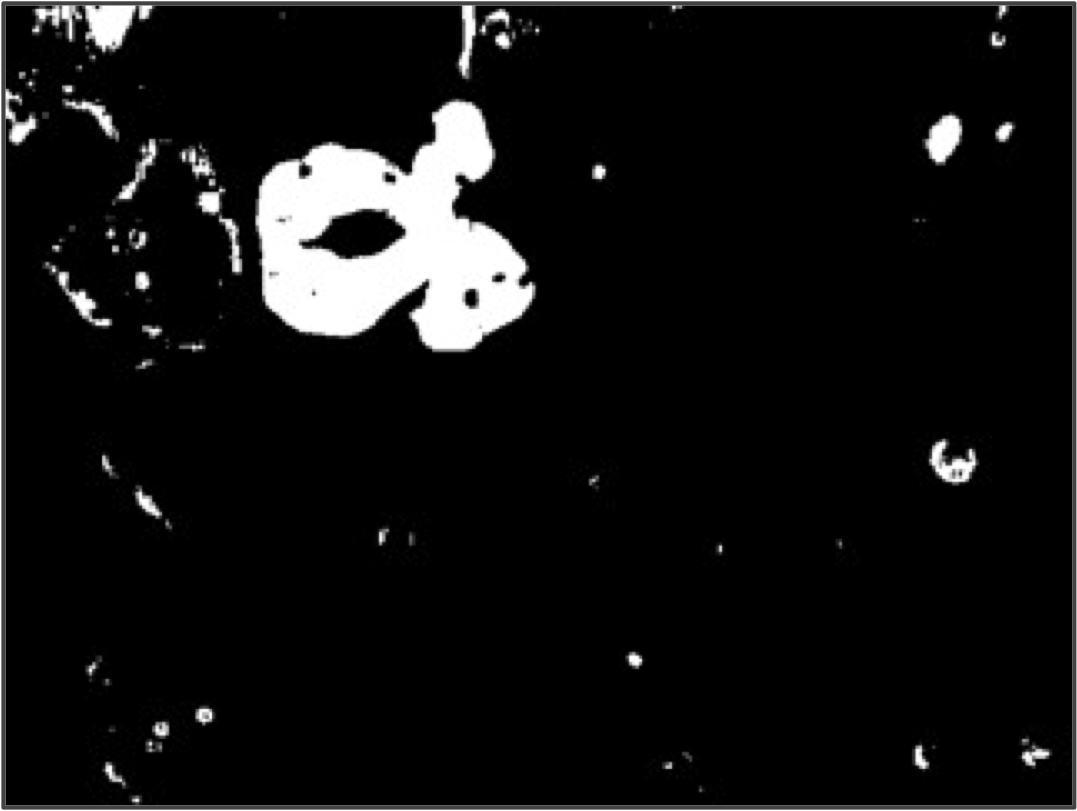
\includegraphics[width = 0.4\textwidth]{../images/neutrophil_binarized_red.png}
\end{tabular}
\caption{Two more binarized versions of the neutrophil image from \autoref{fig:three_families} (left), based on the green and red channels. For both these colors, the WBC nucleus tends to have lower values than other parts of the original image. (Left) A binarization in which a pixel is colored white if it has a green value less than or equal to 153, and a pixel is colored black otherwise. (Right) A binarization in which a pixel is turned white if it has a red value less than or equal to 166, and a pixel is colored black otherwise.}
\label{fig:neutrophil_binarized_other_colors}
\end{figure}

It would seem that we should work with the binarized image based on the red threshold, which contains the clearest image of the nucleus among the three binarized images. However, note that each threshold was successful in eliminating some of the non-nuclear parts of the image. For example, the white regions in the top left of both binarized images in \autoref{fig:neutrophil_binarized_other_colors} was eliminated by the binarized image in \autoref{fig:neutrophil_binarized_blue} based on the blue threshold, which initially did not seem helpful.

This insight gives us an idea: if each of the three binarized images was successful at excluding some part of the image, then let us produce a fourth image in which a pixel is white only if it is white in all three binarized images, and a pixel is black if it is black in any of the three binarized images.\tutorial[white_blood_cells/tutorial_nuclear_segmentation] This process typically produces a nice result, as indicated in \autoref{fig:segmentation} for the sample monocyte and lymphocyte images presented in \autoref{fig:three_families}. At the same time, no segmentation pipeline is perfect; \autoref{fig:segmentation_imperfect} illustrates that for a few images in our dataset, we may not correctly segment the entire nucleus. \\

\begin{figure}[h]
\centering
\tabcolsep = 1em
\mySfFamily
\begin{tabular}{c c}
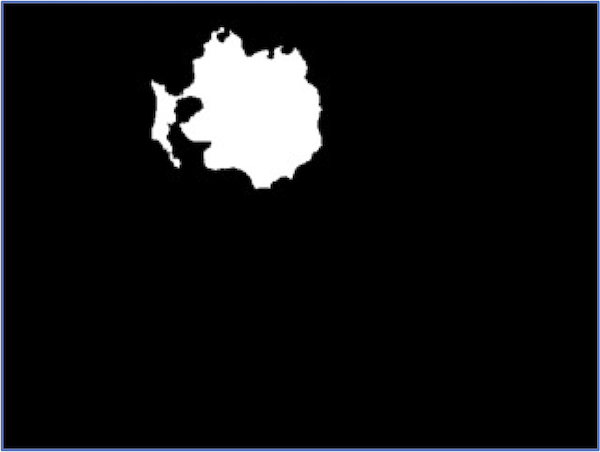
\includegraphics[width = 0.4\textwidth]{../images/monocyte_binarized.png} & 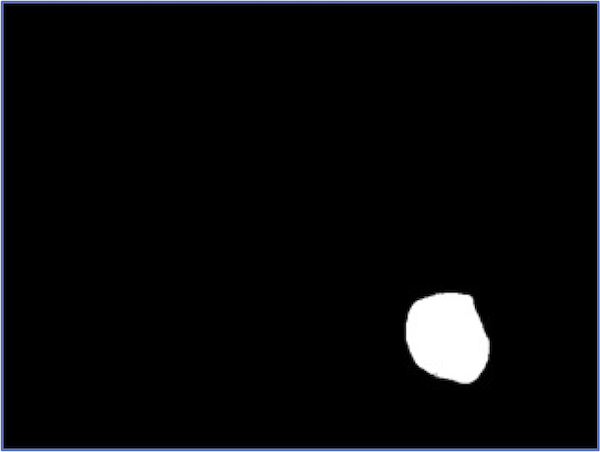
\includegraphics[width = 0.4\textwidth]{../images/lymphocyte_binarized.png}
\end{tabular}
\caption{Image segmentation of the monocyte (left) and lymphocyte (right) from images from \autoref{fig:three_families} (center) and \autoref{fig:three_families} (right), respectively.}
\label{fig:segmentation}
\end{figure}

\begin{figure}[h]
\centering
\tabcolsep = 1em
\mySfFamily
\begin{tabular}{c c}
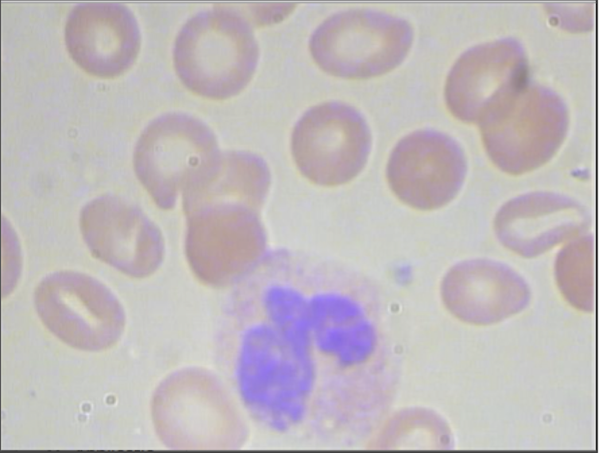
\includegraphics[width = 0.4\textwidth]{../images/WBC_167.png} & 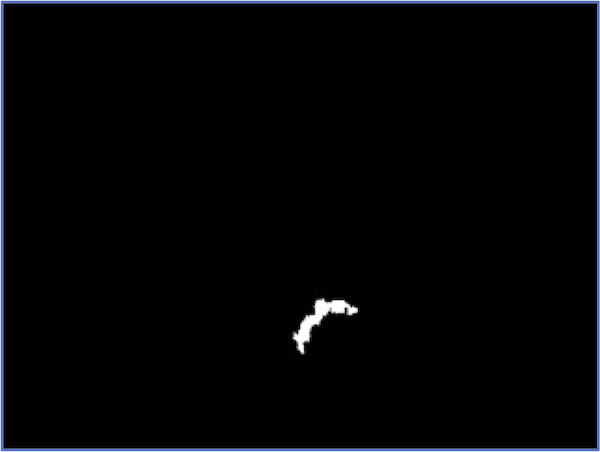
\includegraphics[width = 0.4\textwidth]{../images/WBC_167_segmentation.png}
\end{tabular}
\caption{(Left) An image of a WBC (ID: 167). (Right) The binarization of this image, showing that the nucleus is not correctly identified during segmentation using the parameters described in the text.}
\label{fig:segmentation_imperfect}
\end{figure}

We can continue to tweak threshold parameters, but our relatively simple algorithm successfully segments almost every WBC nucleus from our dataset. We are ready to move on to classify WBC nuclei into families according to their shape.\\



\FloatBarrier
\phantomsection
\section{An Overview of Classification and k-Nearest Neighbors}
\label{sec:knn}


\phantomsection
\subsection{The classification problem and the iris flower dataset}

Categorizing images of WBCs according to family is a specific instance of a ubiquitous problem in data science, in which we wish to \textit{classify} each object in a given dataset into one of \textvar{k} groups called \textdefnogloss{classes}. In our ongoing example, the data are images of WBCs, and the classes are the three main families of WBCs (granulocytes, lymphocytes, and monocytes). To take a different example, our data could be tumor genomes sequenced from cancer patients, which we want to classify according to the therapeutic that should be prescribed for the patient. Or the data may be the past sales behavior of shoppers, whom we wish to classify into two classes based on a prediction of whether they will buy a new product.

A classical dataset used for motivating classification is the \textdef{iris flower dataset}{iris flower dataset}{a dataset commonly used for motivating classification, which was compiled by Edgar Anderson, and which Ronald Fisher used in a seminal paper on classification in 1936}, which was compiled by Edgar Anderson and used by Ronald Fisher in a seminal paper on classification in 1936. Anderson took measurements from 150 iris flowers, fifty from each of three species (\autoref{fig:iris_flowers}).\\

\begin{figure}[h]
\centering
\tabcolsep = 1em
\mySfFamily
\begin{tabular}{c c c}
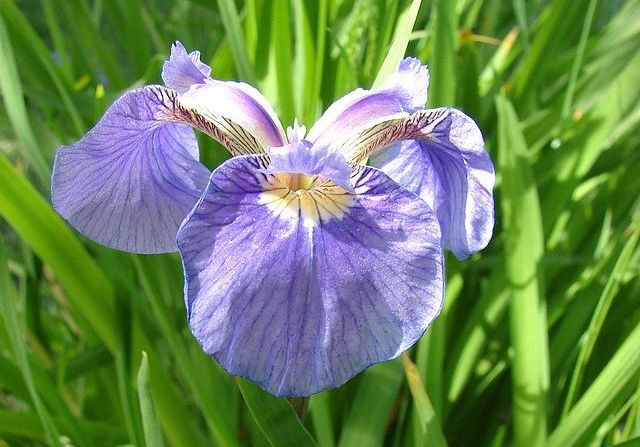
\includegraphics[width = 0.25\textwidth]{../images/Iris_setosa_2.jpg} & 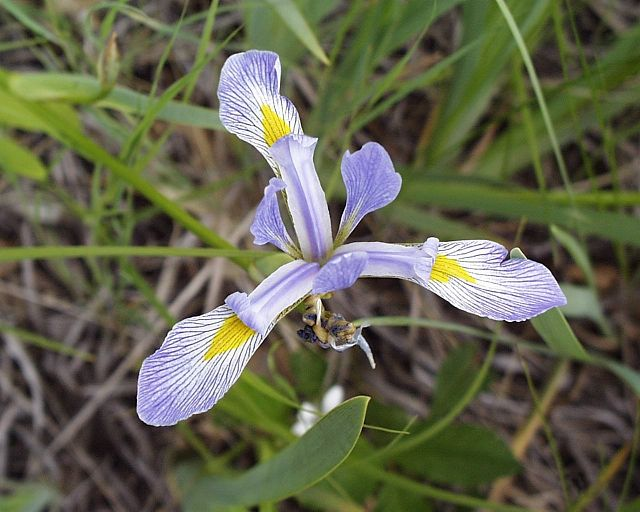
\includegraphics[width = 0.25\textwidth]{../images/Iris_versicolor.jpg} & 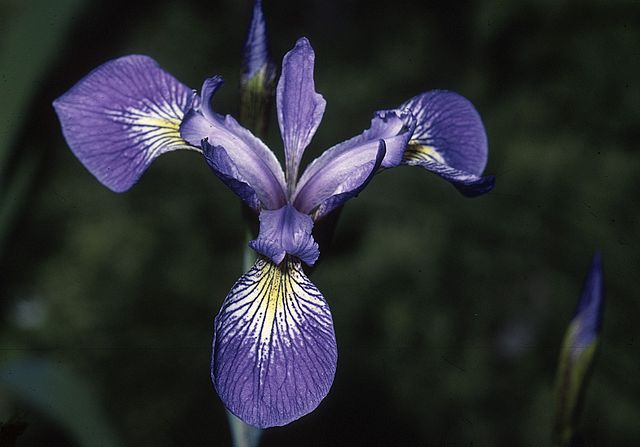
\includegraphics[width = 0.25\textwidth]{../images/Iris_virginica.jpg}
\end{tabular}
\caption{Representative images of the three species of iris included in Anderson's iris flower dataset. (Left) \textit{Iris setosa}. (Center)  \textit{Iris versicolor}. (Right) \textit{Iris virginica}.}
\label{fig:iris_flowers}
\end{figure}

Anderson measured four attributes, or \textdef{features}{feature}{a measurable characteristic of a data point; multiple features are grouped together to form a feature vector in which the \textvar{i}-th element is the data point's value for the \textvar{i}-th feature}, of each flower in his dataset: the width and height of the flower's petal, and the width and height of the flower's sepal (a green offshoot beneath the petals). \autoref{fig:iris_feature_table} shows the features and species labels for twelve of the flowers in the iris flower dataset. Fisher noticed that flowers from the same species had similar features and wondered whether it was possible to classify the flowers according to its species using only Anderson's four features.\\


\begin{figure}[h]
\centering
\tabcolsep = 0.45 em
\mySfFamily
\rowcolors{2}{gray!25}{white}
\begin{tabular}{c c c c c}
\rowcolor{gray!50}
\textbf{Sepal length} & \textbf{Sepal width} & \textbf{Petal length} & \textbf{Petal width} & \textbf{Species} \\
5.1 & 3.5 & 1.4 & 0.2 & \textit{I. setosa} \\
4.9 & 3.0 & 1.4 & 0.2 & \textit{I. setosa} \\
4.7 & 3.2 & 1.3 & 0.2 & \textit{I. setosa} \\
4.6 & 3.1 & 1.5 & 0.2 & \textit{I. setosa} \\
7.0 & 3.2 & 4.7 & 1.4 & \textit{I. versicolor} \\
6.4 & 3.2 & 4.5 & 1.5 & \textit{I. versicolor} \\
6.9 & 3.1 & 4.9 & 1.5 & \textit{I. versicolor} \\
5.5 & 2.3 & 4.0 & 1.3 & \textit{I. versicolor} \\
6.3 & 3.3 & 6.0 & 2.5 & \textit{I. virginica} \\
5.8 & 2.7 & 5.1 & 1.9 & \textit{I. virginica} \\
7.1 & 3.0 & 5.9 & 2.1 & \textit{I. virginica} \\
6.3 & 2.9 & 5.6 & 1.8 & \textit{I. virginica} \\
\end{tabular}
\caption{A table containing values of the four features for twelve members of the iris flower dataset, along with each flower's species. Distances are in centimeters. The complete dataset was accessed from the \href{https://archive.ics.uci.edu/ml/datasets/iris}{University of California, Irvine Machine Learning Repository}.}
\label{fig:iris_feature_table}
\end{figure}

\begin{qbox}[%
What are the typical values of each feature for flowers from each species in \autoref{fig:iris_feature_table}?
]\end{qbox}

\FloatBarrier
\phantomsection
\subsection{From flowers to vectors}

If we were to use only two of the four features in the iris flower dataset, then a flower's feature values \textvar{x} and \textvar{y} could be represented as a point in two-dimensional space $(x, y)$. \autoref{fig:iris_petal_data} shows such a plot for the features of petal length (x-axis) and petal width (y-axis).

\begin{figure}[h]
\centering
\mySfFamily
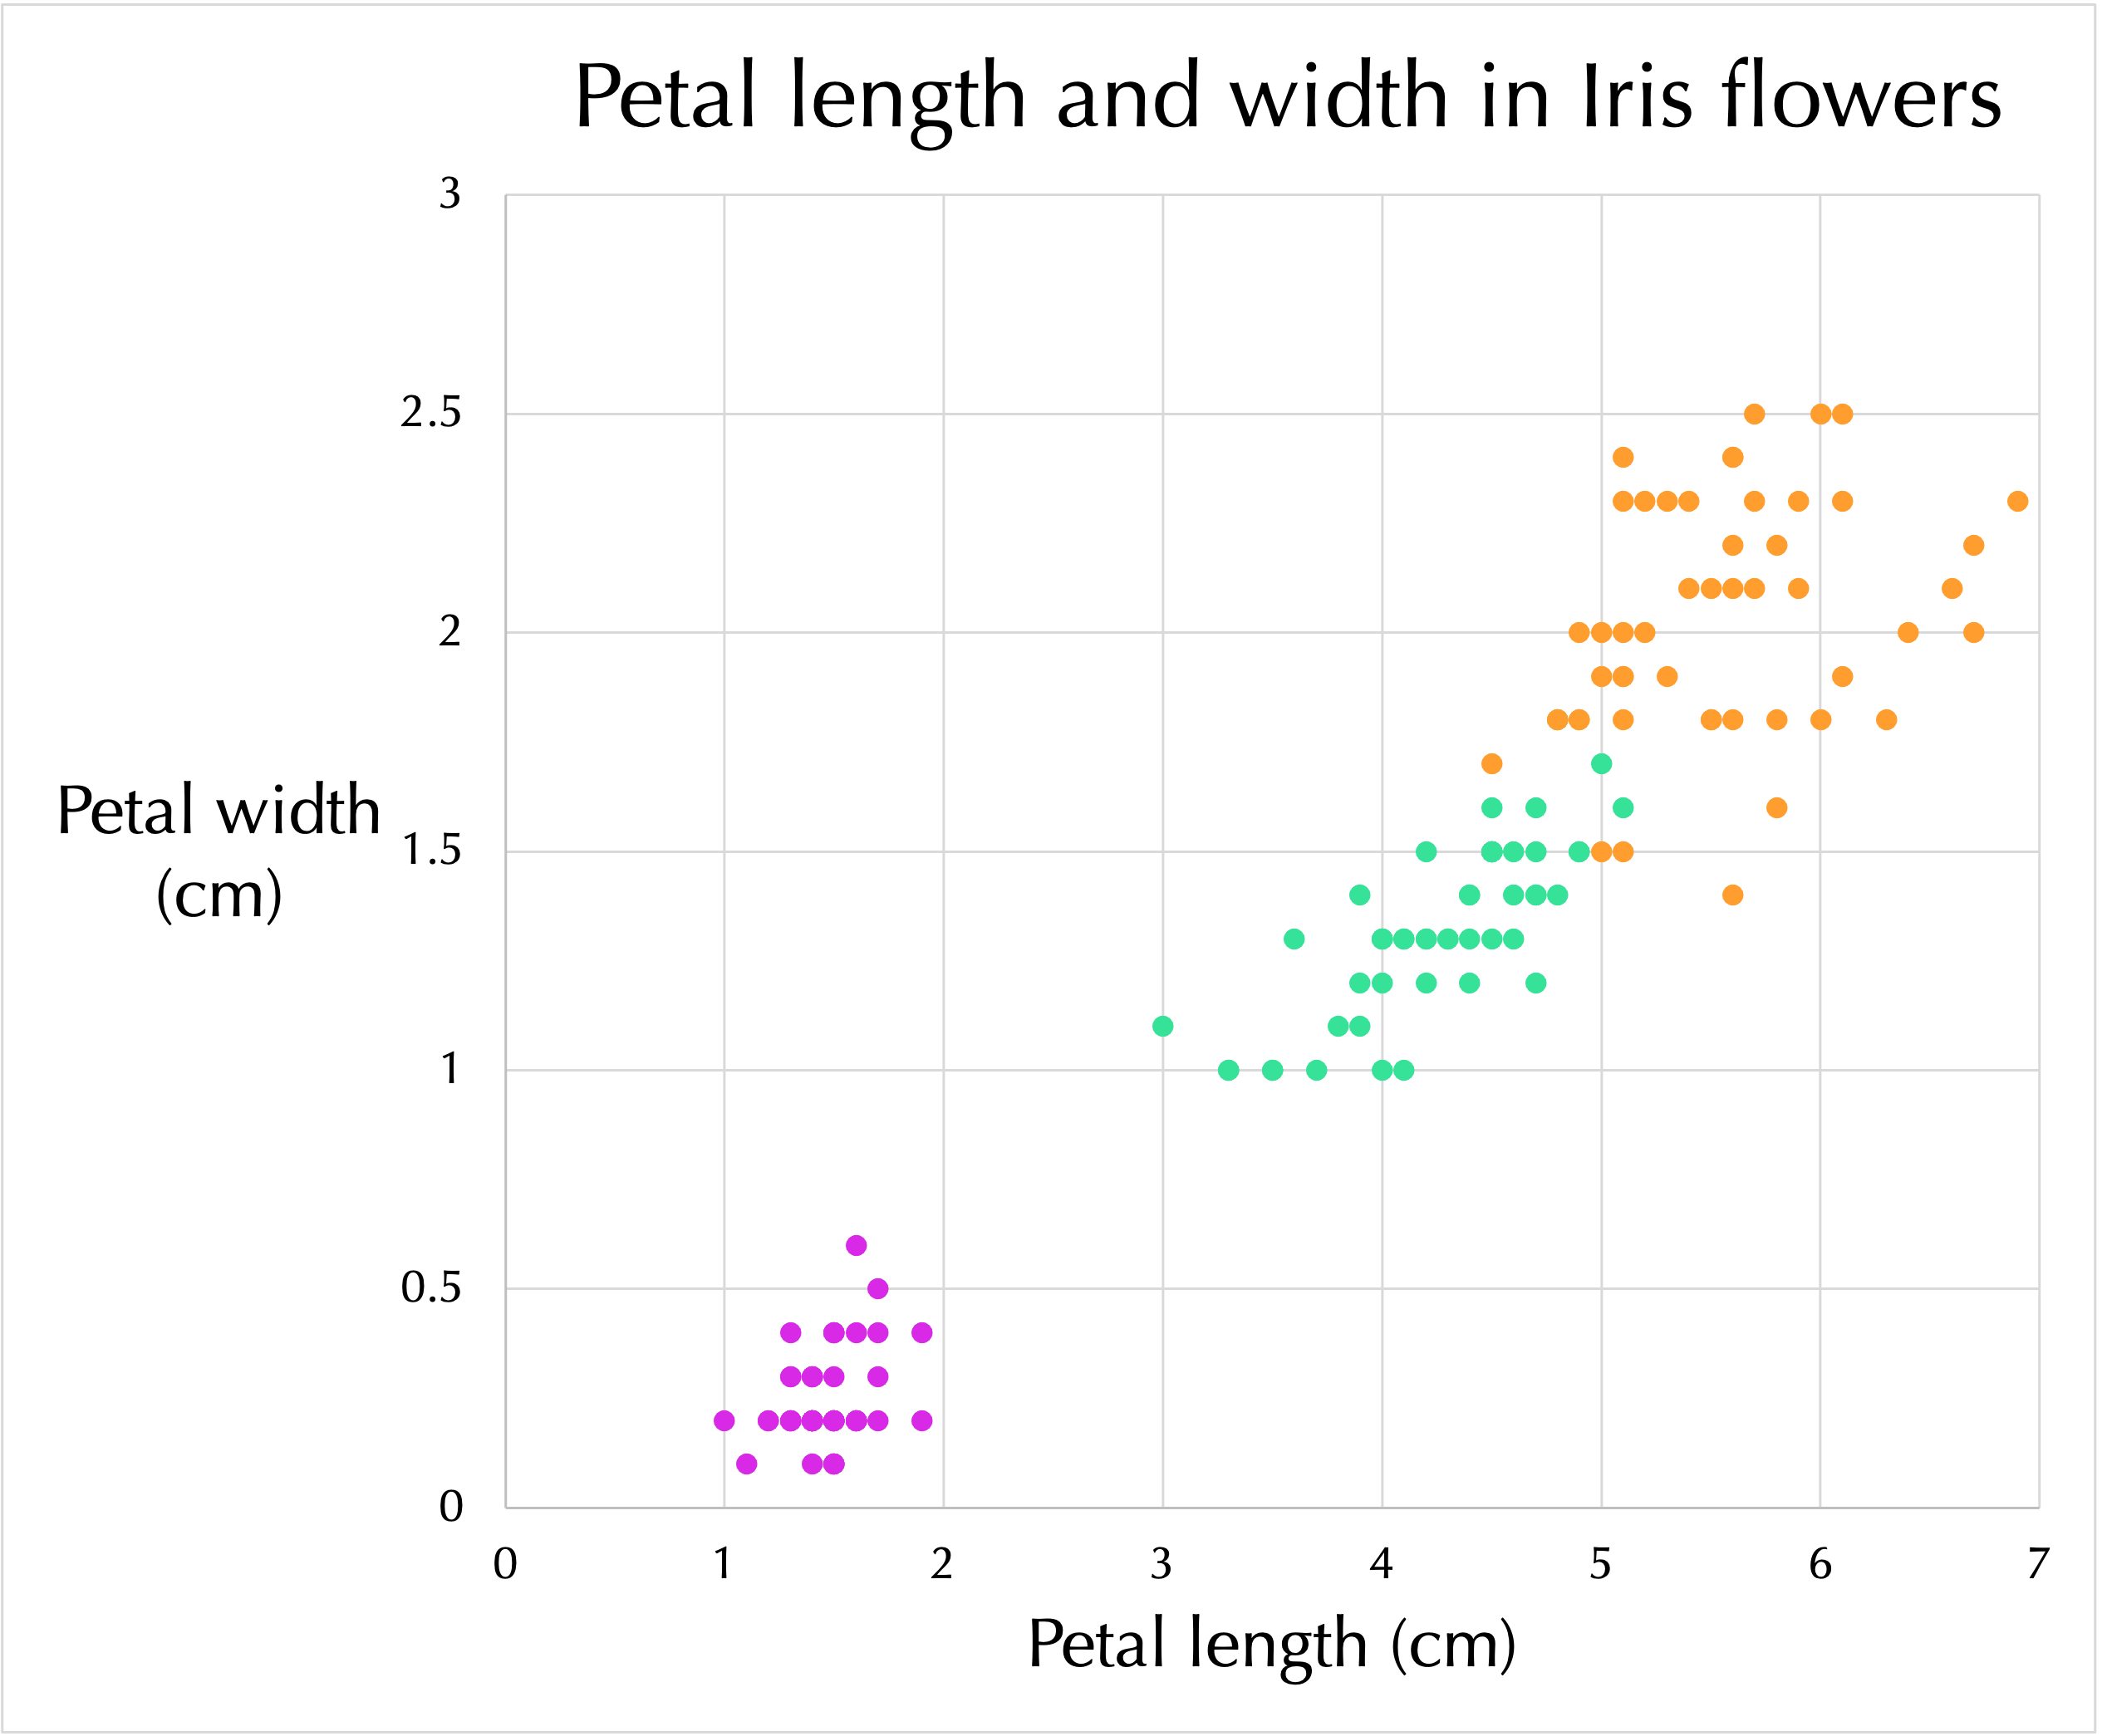
\includegraphics[width = 0.7\textwidth]{../images/iris_petal_data.png}
\caption{Petal width (x-axis) plotted against width (y-axis) for each of the flowers in the iris flower dataset, with data points colored by species. Although there were fifty flowers from each species, there are not fifty points corresponding to every species because some flowers have the same petal length and width and therefore occupy the same point.}
\label{fig:iris_petal_data}
\end{figure}

Note how stark the pattern is in \autoref{fig:iris_petal_data}. Even though we chose only two features from the iris flowers, the points associated with the flowers mostly divide into three main clusters by species. In other words, nearby points tend to correspond to flowers from the same species.

If we were to use all four features for the iris dataset, then every flower would be represented by a point in four-dimensional space. For example, the first flower in our initial table of iris features would be represented by the point $(5.1, 3.5, 1.4, 0.2)$. In general, when classifying a collection of data with \textvar{n} features, each element in the dataset can be represented by a \textdefnogloss{feature vector} of length \textvar{n}, whose \textvar{i}-th value corresponds to the value of the data point's \textvar{i}-th feature.

\FloatBarrier
\phantomsection
\subsection{Classifying unknown elements with k-nearest neighbors}

Our hope is that for datasets other than the iris flower dataset, elements from the same class will have feature vectors that are nearby in \textvar{n}-dimensional space. If so, then we can classify a data point whose class is \textit{unknown} by determining which data points with \textit{known} classification it is near.\\

\begin{qbox}[%
Consider the gray point with unknown class in \autoref{fig:knn_neighborhood}. Should it be assigned to the class of the green points or to the class of the blue points?
]\end{qbox}

\begin{figure}[h]
\centering
\mySfFamily
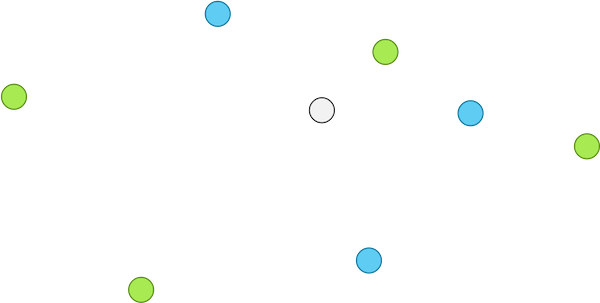
\includegraphics[width = 0.6\textwidth]{../images/knn_neighborhood.png}
\caption{An unknown point (gray) along with a collection of nearby points belonging to two classes, colored green and blue.}
\label{fig:knn_neighborhood}
\end{figure}

The preceding question indicates that classifying points can be surprisingly open-ended. Because of this freedom, researchers have devised a variety of different approaches for classifying data given data with known classes.

We will discuss a simple but powerful classification algorithm called \textdef{k-nearest neighbors (k-NN)}{k-nearest neighbors (k-NN)}{a classification algorithm that assigns each point with unknown class to have the class possessed by the largest number of its \textvar{k} closest neighbors with known class}. In k-NN, we fix a positive integer \textvar{k} in advance. Then, for each point with unknown class, we assign it to the class possessed by the largest number of its \textvar{k} closest neighbors.

In the ongoing example, if we were using \textvar{k} equal to 1, then we would assign the unknown point from \autoref{fig:knn_neighborhood} to the green class (\autoref{fig:knn_neighborhood_k=1}). However, with the same data and \textvar{k} equal to 4, most of the gray point's \textvar{k} nearest neighbors are blue, and so we classify the unknown point as blue (\autoref{fig:knn_neighborhood_k=4}). This example reinforces a theme of this course, that the results of an algorithm can be sensitive to our choice of parameters.\\

\begin{figure}[h]
\centering
\mySfFamily
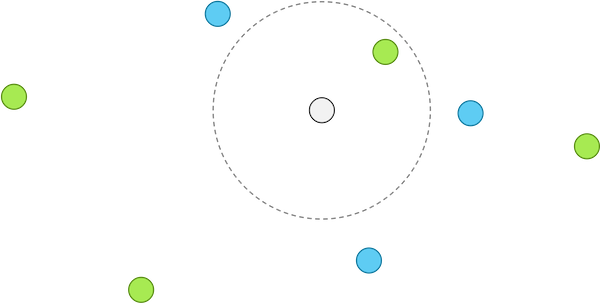
\includegraphics[width = 0.6\textwidth]{../images/knn_neighborhood_k=1.png}
\caption{When \textvar{k} is equal to 1, k-NN classifies an unknown point according to the point of known class that is nearest; for this reason, the gray point with unknown class would be assigned to the green class. (Bottom)}
\label{fig:knn_neighborhood_k=1}
\end{figure}

\begin{figure}[h]
\centering
\mySfFamily
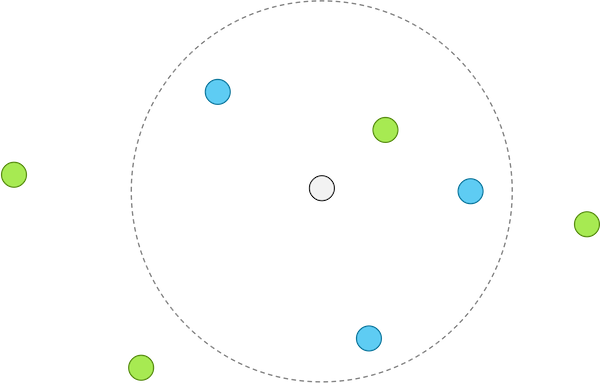
\includegraphics[width = 0.6\textwidth]{../images/knn_neighborhood_k=4.png}
\caption{When \textvar{k} is equal to 4, k-NN classifies the gray point as blue, since three of its four closest neighbors are blue.}
\label{fig:knn_neighborhood_k=4}
\end{figure}

\begin{qbox}[%
When \textvar{k} is equal to 2 or 6 for the classification of the point in \autoref{fig:knn_neighborhood}, note that we obtain a tie in the number of points from each known class belonging to the \textvar{k} nearest neighbors of a point with unknown class. How could we break ties in k-NN?
]\end{qbox}

In the more general case in which feature vectors have \textvar{n} coordinates, we can determine which points are nearest to a given point by using the \textdefnogloss{Euclidean distance}, which generalizes the distance formula to handle vectors in \textvar{n}-dimensional space. The Euclidean distance between vectors $\mathbf{x} = (x_1, x_2, \ldots, x_n)$ and $\mathbf{y} = (y_1, y_2, \ldots, y_n)$ is given by the sum of squares of differences between corresponding vector elements:

$$d(\mathbf{x}, \mathbf{y}) = \sqrt{(x_1 - y_1)^2 + (x_2 - y_2)^2 + \cdots + (x_n-y_n)^2}\,.$$

We now have learned how to use k-NN to classify feature vectors with unknown classes given vectors with known classes. There is just one problem: how can we convert an image of a WBC into a vector?\\

\FloatBarrier
\phantomsection

\section{Shape Spaces}
\label{sec:shape_spaces}
\phantomsection

\subsection{Interlude: Stone tablets and lost cities}

Imagine that you are an interstellar traveler to Earth and come across the ruins of New York City. You find an old road atlas that has driving distances between cities (\autoref{fig:atlas}). Can you use this atlas to find the other cities? In \autoref{chapter:chemotaxis}, we encountered a ``Lost Immortals'' problem; we call the problem of inferring the locations of cities given the distance between them the ``Lost Cities'' problem.\\

\begin{figure}[h]
\centering
\tabcolsep = 0.7 em
\mySfFamily
\small
\rowcolors{2}{gray!25}{white}
\begin{tabular}{r c c c c c c}
\rowcolor{gray!50}
& \textbf{NYC} & \textbf{LA} & \textbf{Pitt.} & \textbf{Miami} & \textbf{Houston} & \textbf{Seattle} \\
\textbf{New York City} & 0 & 2805 & 371 & 1283 & 1628 & 2852 \\
\textbf{Los Angeles} & 2805 & 0 & 2427 & 2733 & 1547 & 1135 \\
\textbf{Pittsburgh} & 371 & 2427 & 0 & 1181 & 1388 & 2502 \\
\textbf{Miami} & 1283 & 2733 & 1181 & 0 & 1189 & 3300 \\
\textbf{Houston} & 1628 & 1547 & 1388 & 1189 & 0 & 2340 \\
\textbf{Seattle} & 2852 & 1135 & 2502 & 3300 & 2340 & 0 \\
\end{tabular}
\caption{All pairwise distances (in miles) between six cities in the United States.}
\label{fig:atlas}
\end{figure}

\begin{qbox}[%
If you know the location of New York, how could you use the information in \autoref{fig:atlas} to find the other cities?
]\end{qbox}

This seemingly contrived example has a real archaeological counterpart. In 2019, researchers used commercial records that had been engraved by Assyrian merchants onto 19th Century BCE stone tablets in order to estimate distances between pairs of Bronze age cities in present-day Turkey. Using this ``atlas'' of sorts, they estimated the locations of lost cities.

You may be confused as to why biologists should care about stone tablets and lost cities. Let us therefore return to our problem of classifying segmented WBC images by family.

\FloatBarrier
\phantomsection
\subsection{Vectorizing a segmented image}

We would like to apply a classification algorithm like k-NN to our example of segmented WBC images. Yet k-NN first requires each object to be represented by a feature vector, and so we need some way of converting a WBC image into a feature vector. In this way, we can produce a \textdef{shape space}{shape space}{an assignment of shapes to points in multi-dimensional space}, or an assignment of shapes to points in multi-dimensional space.

You may notice that the problem of ``vectorizing'' a WBC image is similar to one that we have already encountered in \autoref{chapter:coronavirus}, when we vectorized a protein structure \textvar{S} as the collection of locations of its \textvar{n} alpha carbons to produce a vector $\mathbf{s} = (s_1, \ldots, s_n)$, where $s_i$ is the position of the \textvar{i}-th alpha carbon of \textvar{S}.

We will apply the same idea to vectorize our segmented WBCs. Given a binarized WBC nucleus image, we will first center the image so that its center of mass is at the origin, and then sample \textvar{n} points from the boundary of the cell nucleus to produce a \textdef{shape vector}{shape vector}{a feature vector for a shape whose features are points on the boundary of the shape} $s = (s_1, \ldots, s_n)$, where $s_i$ is a point with coordinates $(x(i), y(i))$.\\

\begin{note}[%
Both identifying the boundary of a binarized image and sampling points from this boundary to ensure that points are similarly spaced are challenging tasks that are outside the scope of our work here, and which we will let modeling software handle for us.
]\end{note}

To determine the ``distance'' between two images' shape vectors, we will use our old friend root mean square deviation (RMSD), which is very similar to the Euclidean distance. Given shape vectors $\mathbf{s}$ and $\mathbf{t}$, the RMSD between these vectors is

$$\text{RMSD}(\mathbf{s}, \mathbf{t}) = \sqrt{\dfrac{1}{n} \cdot (d(s_1, t_1)^2 + d(s_2, t_2)^2 + \cdots + d(s_n, t_n)^2)}\,. $$

\FloatBarrier
\phantomsection
\subsection{Inferring a shape space from pairwise distances}

It is tempting to take the vectorization of every shape as our desired shape space. If this were the case, then we would hope that images of similarly shaped nuclei will have low RMSD and that the more dissimilar two nuclei become, the higher the RMSD of their shape vectors. The potential issues with this assumption are the same as those encountered when discussing protein structures, which we now review.

On the one hand, recall the danger from undersampling from \autoref{fig:circle_square_undersampling}, so that we must ensure that the number of points that we sample from the object boundary is sufficiently high to avoid dissimilar shapes from having low RMSD. On the other hand, we could have very similar shapes whose RMSD winds up being high. For example, recall the shapes in \autoref{fig:two_shapes}, which are identical, but one has been flipped and rotated. If we were to vectorize these shapes as they are now in the same way (say, by starting at the top of the shape and proceeding clockwise), then we would obtain two vectors with high RMSD.

We handled the latter issue in our work on protein structure comparison by introducing the Kabsch algorithm, which identified the best rotation of one shape into another that would minimize the RMSD of the resulting shape vectors. And yet what makes our work here more complicated is that we are not comparing  two WBC image shape vectors, we are comparing hundreds.

However, we could apply the Kabsch algorithm to every pair of images, producing the RMSD between every pair of images. We would then need to build a shape space from all these distances between pairs of shapes. We hope that this problem sounds familiar, as it is the Lost Cities problem in disguise. The pairs of distances between images correspond to a road atlas, and placing images into a shape space corresponds to locating cities.

Statisticians have devised a collection of approaches called multi-dimensional scaling to solve versions of the Lost Cities problem that arise frequently in practice. The fundamental idea of multi-dimensional scaling is to assign points to \textvar{n}-dimensional space such that the distances between points in this space approximately resemble a collection of distances between pairs of objects in some dataset.\\

\begin{qbox}[%
If we have \textvar{m} cellular images, then how many times will we need to compute the distance between a pair of images?
]\end{qbox}

\FloatBarrier
\phantomsection
\subsection{Aligning many images concurrently}

Unfortunately, if we have a large dataset, then computing the distance between every pair of objects can prove time-intensive, even with a powerful computer. Instead, we will rotate all images \textit{concurrently}. After this alignment, we can then center and vectorize all the images starting at the same position.

One way of aligning a collection of images is to first identify the \textdef{major axis}{major axis}{the line segment crossing through an object's center of mass that is as long as possible} of each image, which is the line segment crossing through the image's center of mass that is as long as possible. \autoref{fig:three_similar_shapes_unaligned} shows the major axis for a few similar shapes.\\

\begin{figure}[h]
\centering
\mySfFamily
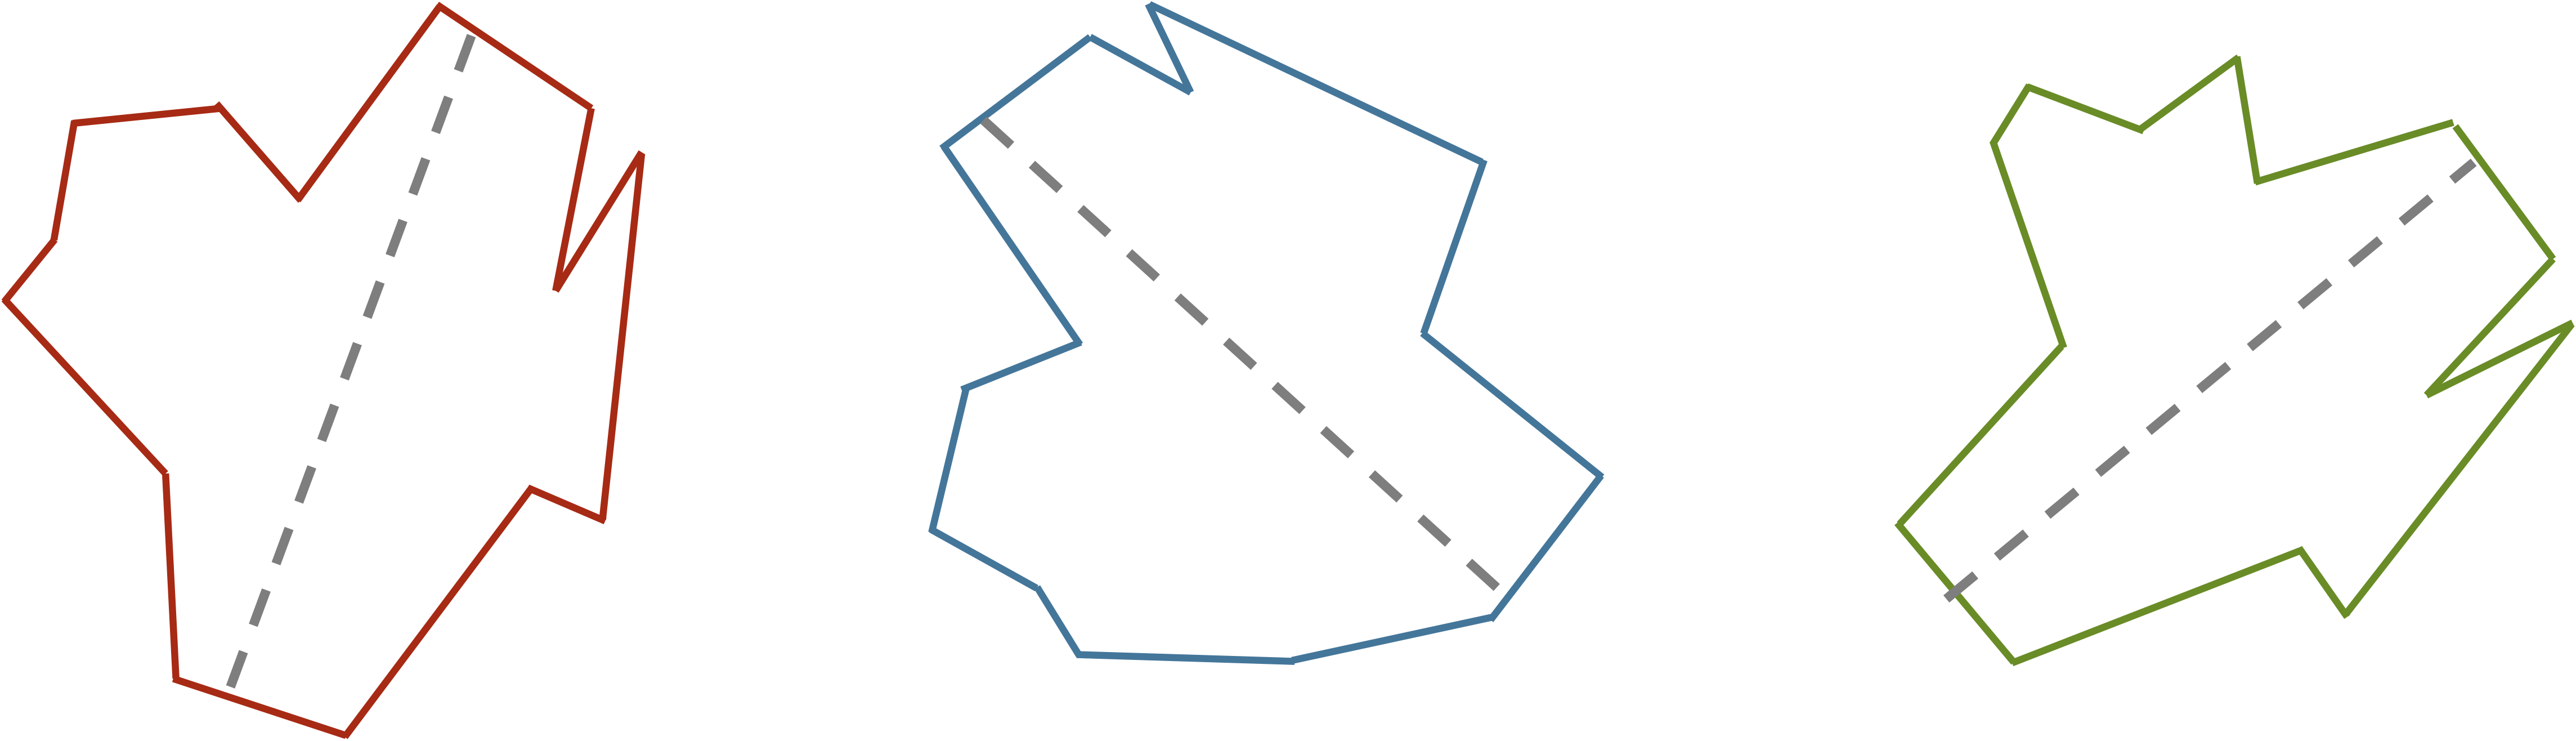
\includegraphics[width = 0.85\textwidth]{../images/three_similar_shapes_unaligned.png}
\caption{Three similar shapes, with their major axes highlighted in gray.}
\label{fig:three_similar_shapes_unaligned}
\end{figure}

Aligning the major axes of these similar shapes reveals their similarities (\autoref{fig:three_similar_shapes_aligned}). These images are ready to be vectorized (say, starting from the point on the right side of an image's major axis and proceeding counterclockwise). The resulting vectors will have low RMSD because corresponding points on the shapes will be nearby.\\

\begin{figure}[h]
\centering
\mySfFamily
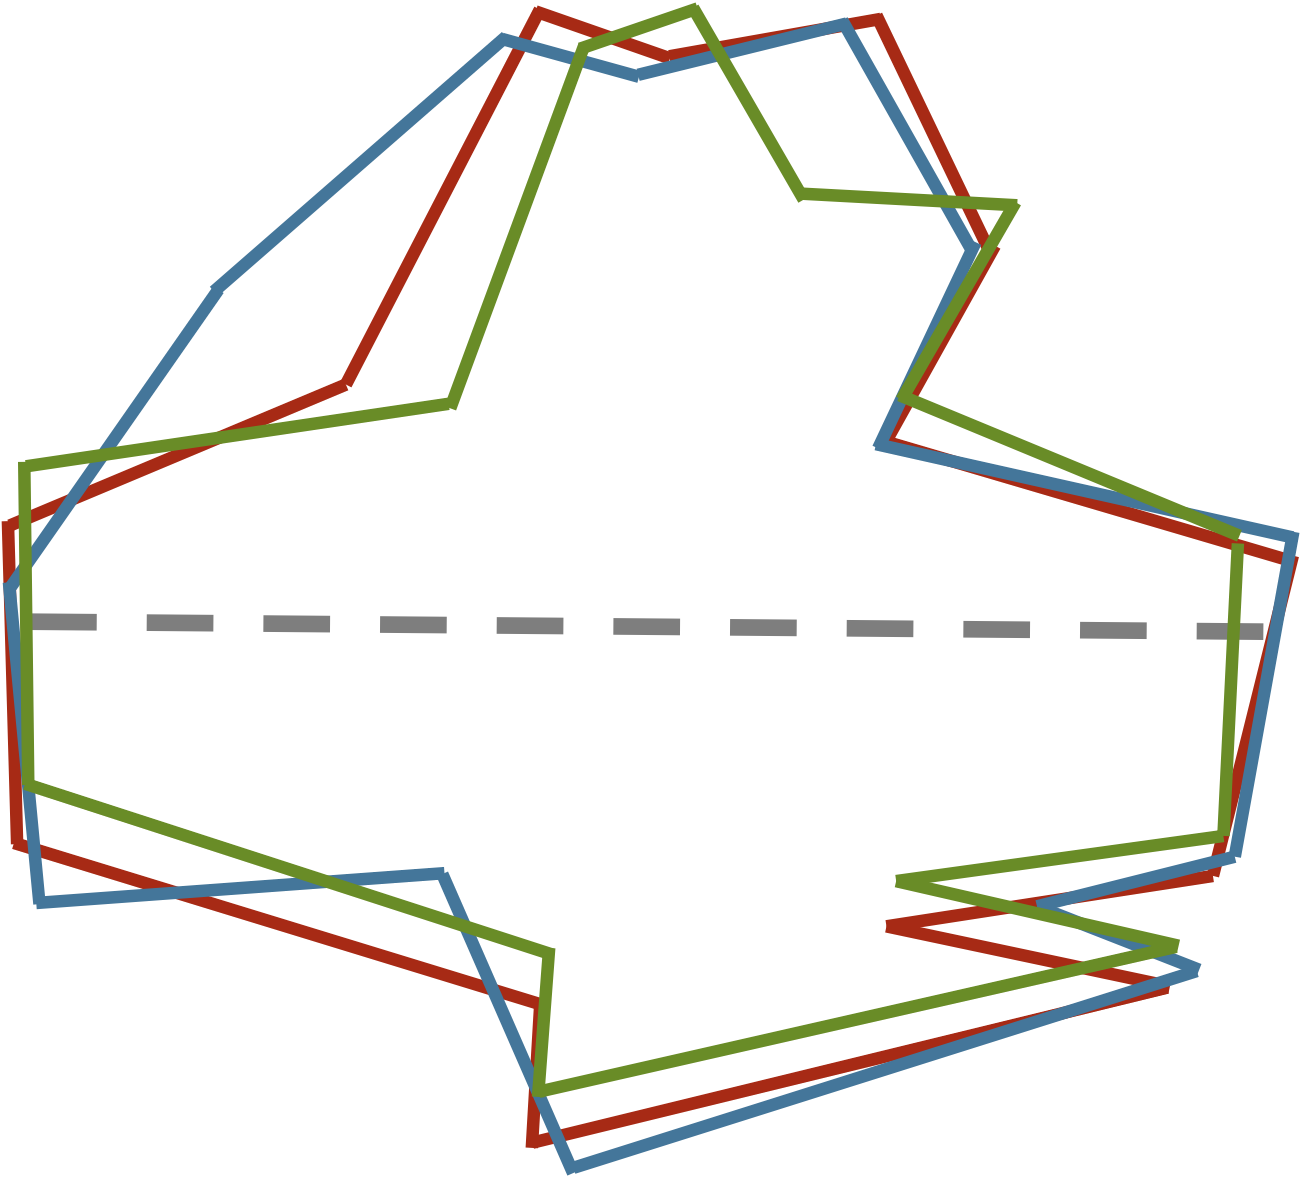
\includegraphics[width = 0.3\textwidth]{../images/three_similar_shapes_aligned.png}
\caption{Aligning the three images from \autoref{fig:three_similar_shapes_unaligned} so that their major axes overlap allows us to see similarities between the shapes as well as build consistent shape vectors for them.}
\label{fig:three_similar_shapes_aligned}
\end{figure}

\begin{note}[%
In practice, when we align shapes along their major axes, we need to consider the flip of each shape across its major axis as well.
]\end{note}

By aligning and then vectorizing a collection of binarized cellular images after alignment, the resulting feature vectors form our desired shape space. We are almost ready to apply a classifier to this shape space, but one more pitfall remains.\\


\FloatBarrier
\phantomsection

\section{Principal Components Analysis}
\label{sec:pca}

\phantomsection
\subsection{The curse of dimensionality}

Things get weird in multi-dimensional space.

Consider a circle inscribed in a square (\autoref{fig:inscribed_circle_and_sphere} (left)). The ratio of the area of the circle to the area of the square is $\pi/4 \approx 0.785$, regardless of the side length. When we move to three dimensions and have a sphere inscribed in a cube (\autoref{fig:inscribed_circle_and_sphere} (right)), the ratio of the volume of the sphere to that of the cube is $(4\pi/3)/8 \approx 0.524$.\\

\begin{figure}[h]
\centering
\mySfFamily
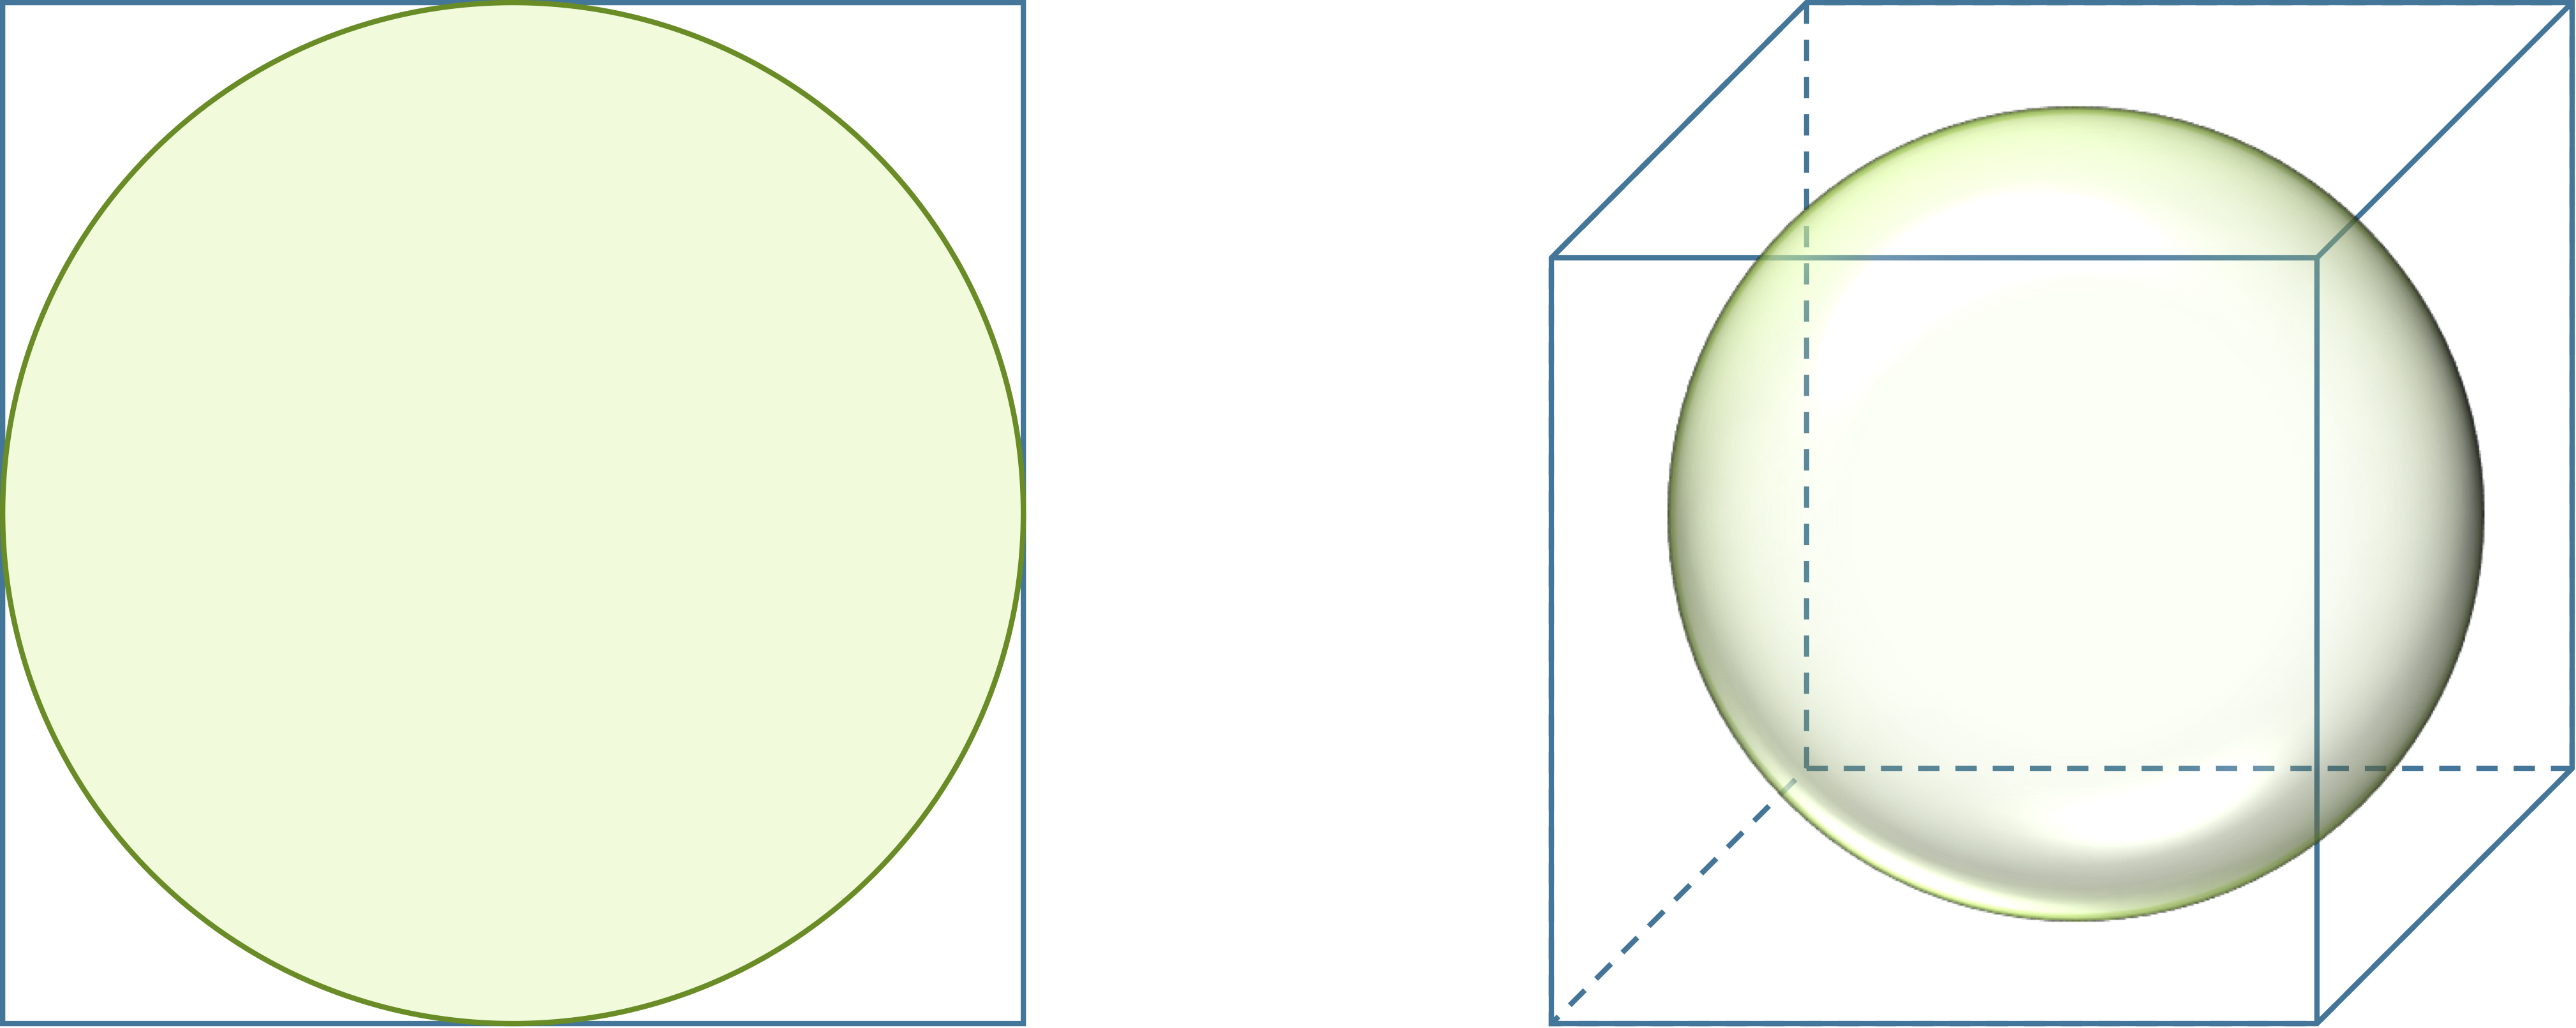
\includegraphics[width = 0.8\textwidth]{../images/inscribed_circle_and_sphere.png}
\caption{A circle inscribed in a square takes up more of the square (78.5 percent) than a sphere inscribed in a cube (52.4 percent).}
\label{fig:inscribed_circle_and_sphere}
\end{figure}

We define an \textvar{n}-dimensional unit sphere as the set of points in \textvar{n}-dimensional space whose Euclidean distance from the origin is at most 1, and an \textvar{n}-dimensional cube as the set of points whose coordinates are all between 0 and 1. A precise definition of the volume of a multi-dimensional object is beyond the scope of this work, but as \textvar{n} increases, the sphere takes up less and less of the cube. As \textvar{n} tends toward infinity, the ratio of the volume of the \textvar{n}-dimensional unit sphere to the volume of the \textvar{n}-dimensional unit cube approaches zero!

One way of interpreting the vanishing of the sphere's volume is that as \textvar{n} increases, an \textvar{n}-dimensional cube has more and more corners in which there points can hide away from the sphere. Most of the cube's volume therefore winds up scattering outward from its center.

The case of the vanishing sphere may seem like an arcane triviality that only holds interest for mathematicians toiling in fluorescently lit academic offices at strange hours. Yet this phenomenon is just one manifestation of a profound paradigm in data science called the \textdef{curse of dimensionality}{curse of dimensionality}{a collection of principles that arise in higher dimensions that run counter to our intuition about three-dimensional space}, a collection of principles that arise in higher dimensions that run counter to our intuition about three-dimensional space.

\FloatBarrier
\phantomsection
\subsection{How the curse of dimensionality affects classification}

In the previous section, we discussed sampling \textvar{n} points from the boundary of a two-dimensional WBC nuclear image, thus converting the image into a vector in a space with $2n$ dimensions. We argued that \textvar{n} needs to be sufficiently large to ensure that comparing the vectors of two images will give an accurate representation of how similar their shapes are. Yet increasing \textvar{n} means that we need to be careful about the curse of dimensionality.

Say that we sample \textvar{k} points randomly from the interior of an \textvar{n}-dimensional unit cube. Let $d_{\text{min}}$ and $d_{\text{max}}$ denote the minimum and maximum distance from any of our points to the origin, respectively. As \textvar{n} grows, the ratio $d_{\text{min}}/d_{\text{max}}$ heads toward 1; in other words, as points fly toward the many corners of the cube, the minimum distance between points becomes indistinguishable from the maximum distance between points.

This other facet of the curse of dimensionality means that algorithms like k-NN, which classify points with unknown classes based on nearby points with known classes, may not perform well in higher-dimensional spaces in which even similar points tend to fly away from each other.

Because of the curse of dimensionality, it makes sense to reduce the number of dimensions before performing any further analysis such as classification. We could reduce the number of features used for generating a vector, especially if we have reason to believe that some features are more informative than others. This approach will likely not work for our WBC image example, since it is not clear why one point on the boundary of our images would be inherently better than another.

Instead, we will reduce the number of dimensions of our shape space without removing any features from the data. As perplexing as multi-dimensional space may already seem, it may be totally unclear how we could reduce the dimensions of a space. We will therefore explain dimension reduction in the context of three-dimensional space; our approach may be more familiar than you think.

\FloatBarrier
\phantomsection
\subsection{Dimension reduction with principal components analysis}

We will introduce dimension reduction using the iris flower dataset. Although this dataset has four features, we will focus again on only petal length and width, which we plot against each other in \autoref{fig:iris_petal_data_unlabeled}. We can trust our eyes to notice the clear pattern: as iris petal width increases, petal length tends to increase as well.\\

\begin{figure}[h]
\centering
\mySfFamily
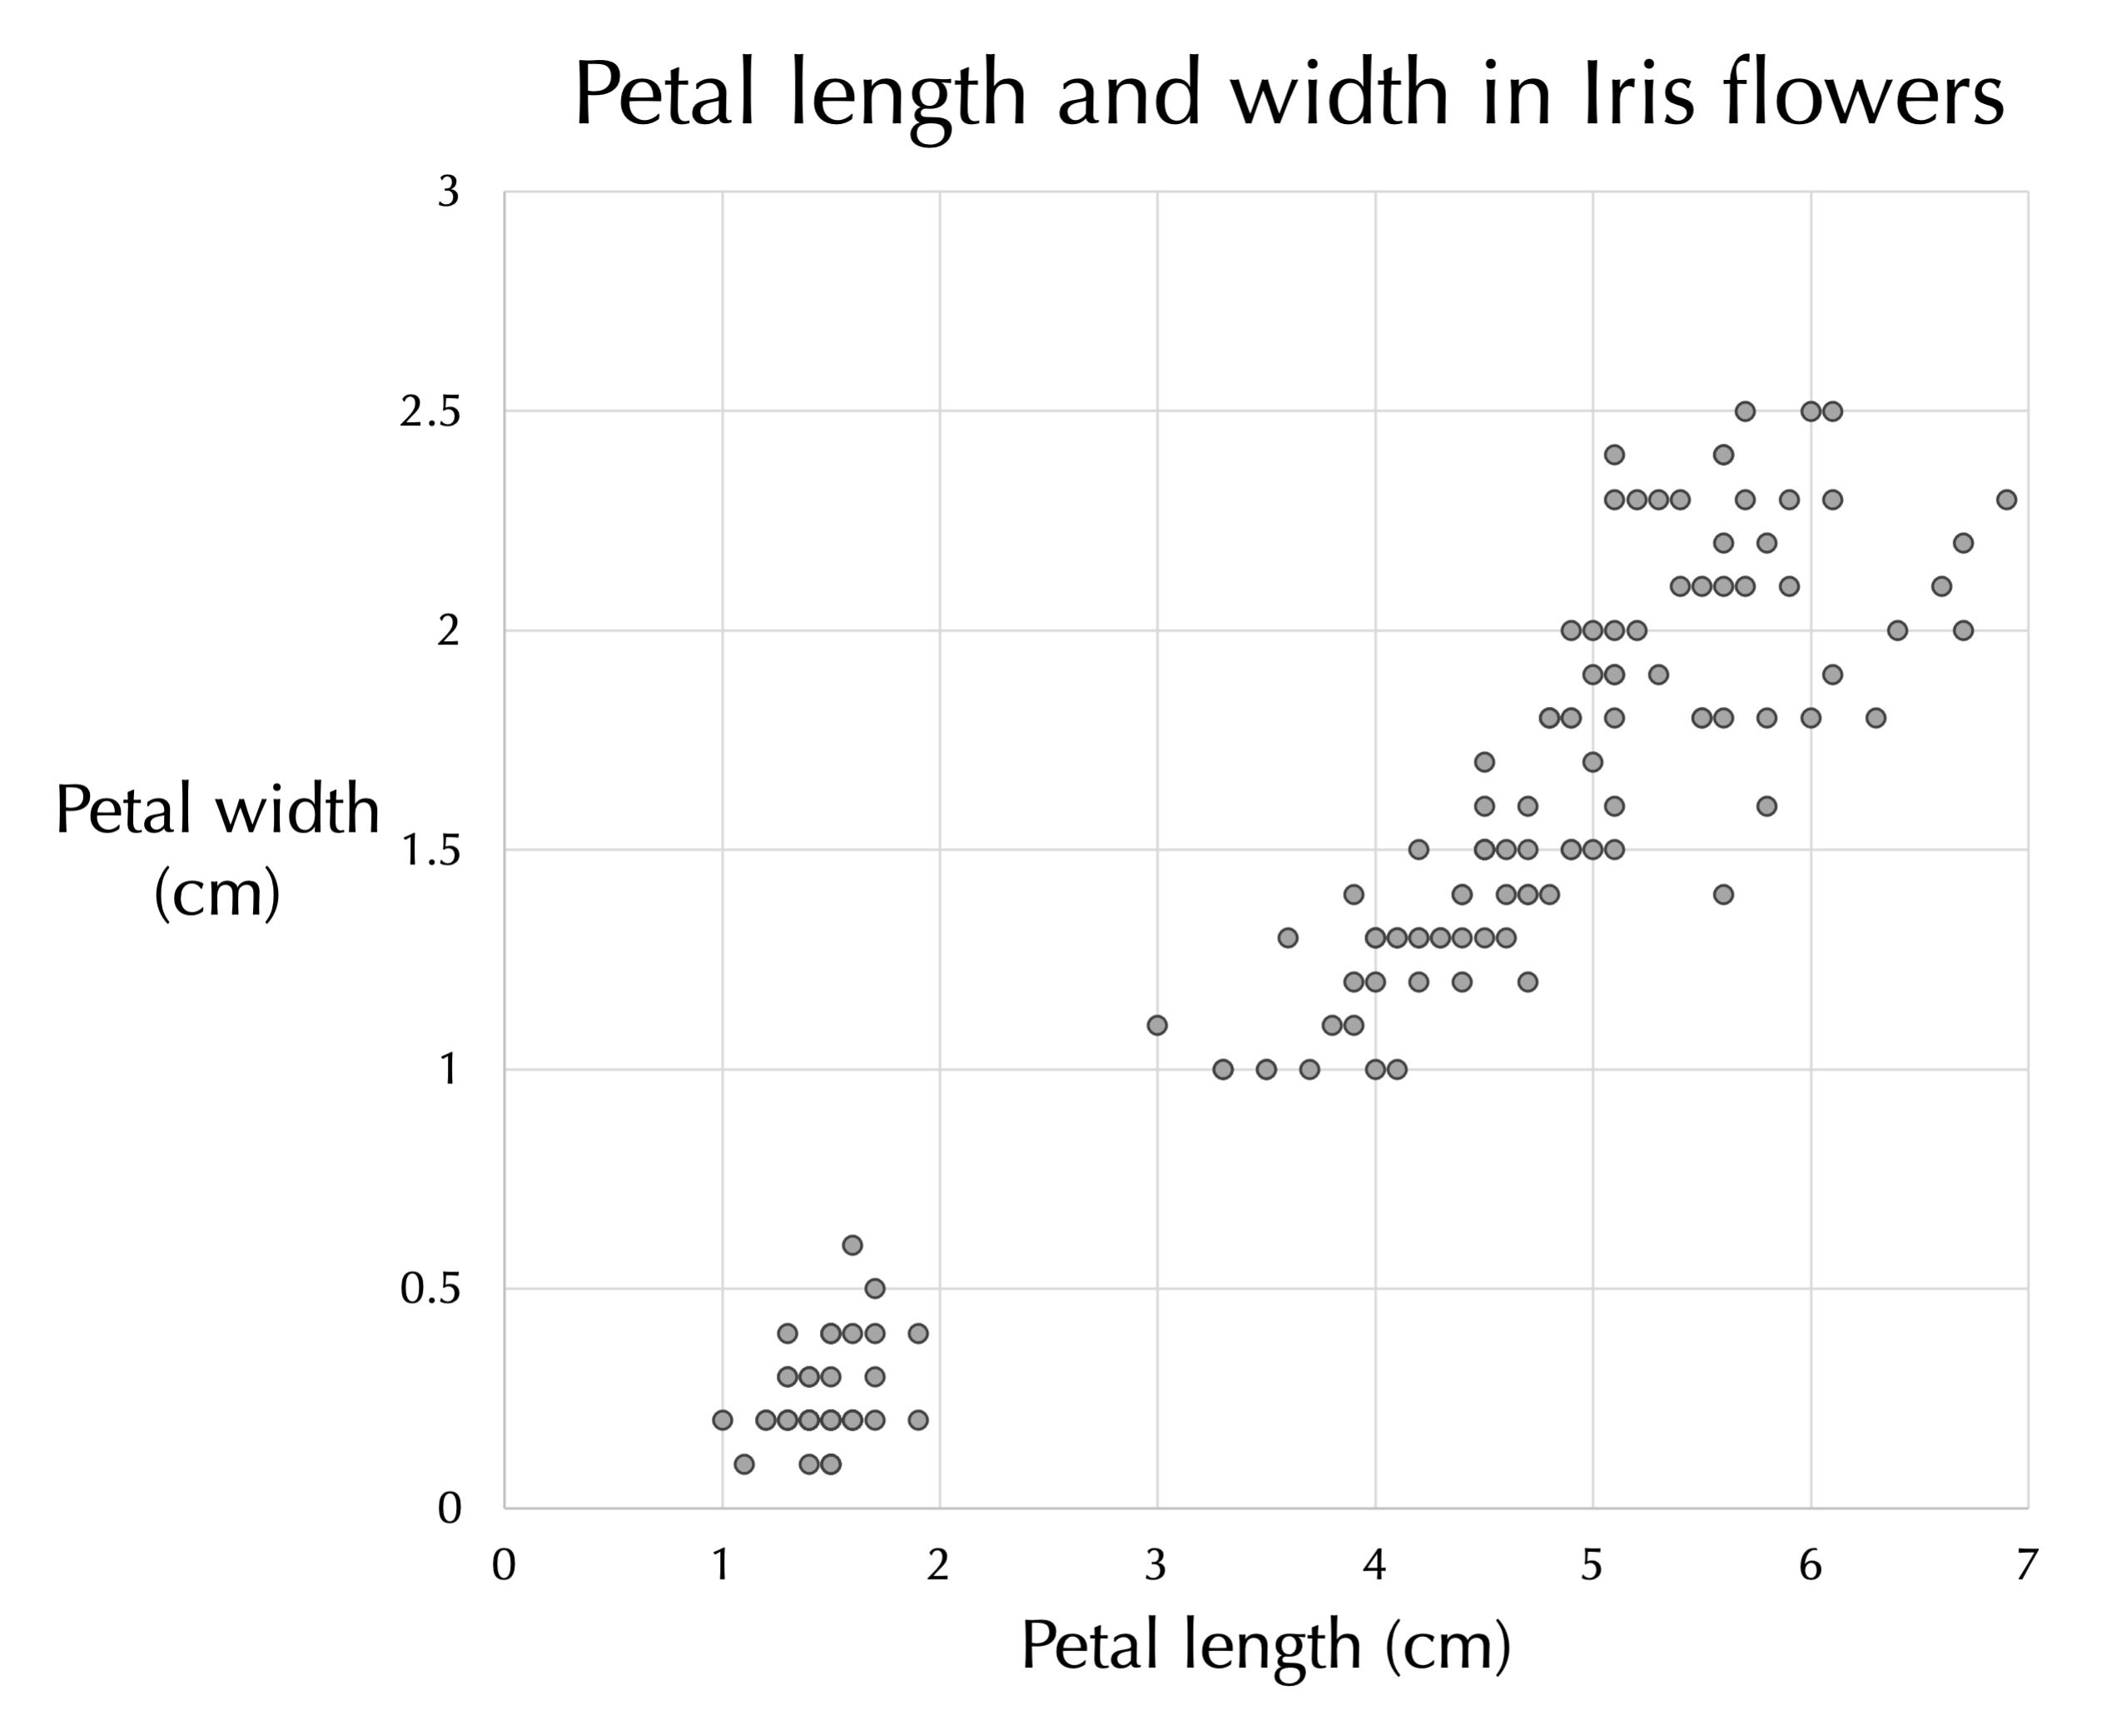
\includegraphics[width = 0.7\textwidth]{../images/iris_petal_data_unlabeled.png}
\caption{Petal width (x-axis) plotted against petal width (y-axis) for all flowers in the iris flower dataset, not labeled according to species.}
\label{fig:iris_petal_data_unlabeled}
\end{figure}

If we draw a line through the center of the data (\autoref{fig:iris_flowers_regression_line}), then the line provides a reasonable estimate of a flower's petal width given its length, and vice-versa. This line, a one-dimensional object, therefore approximates a collection of points in two dimensions.\\

\begin{figure}[h]
\centering
\mySfFamily
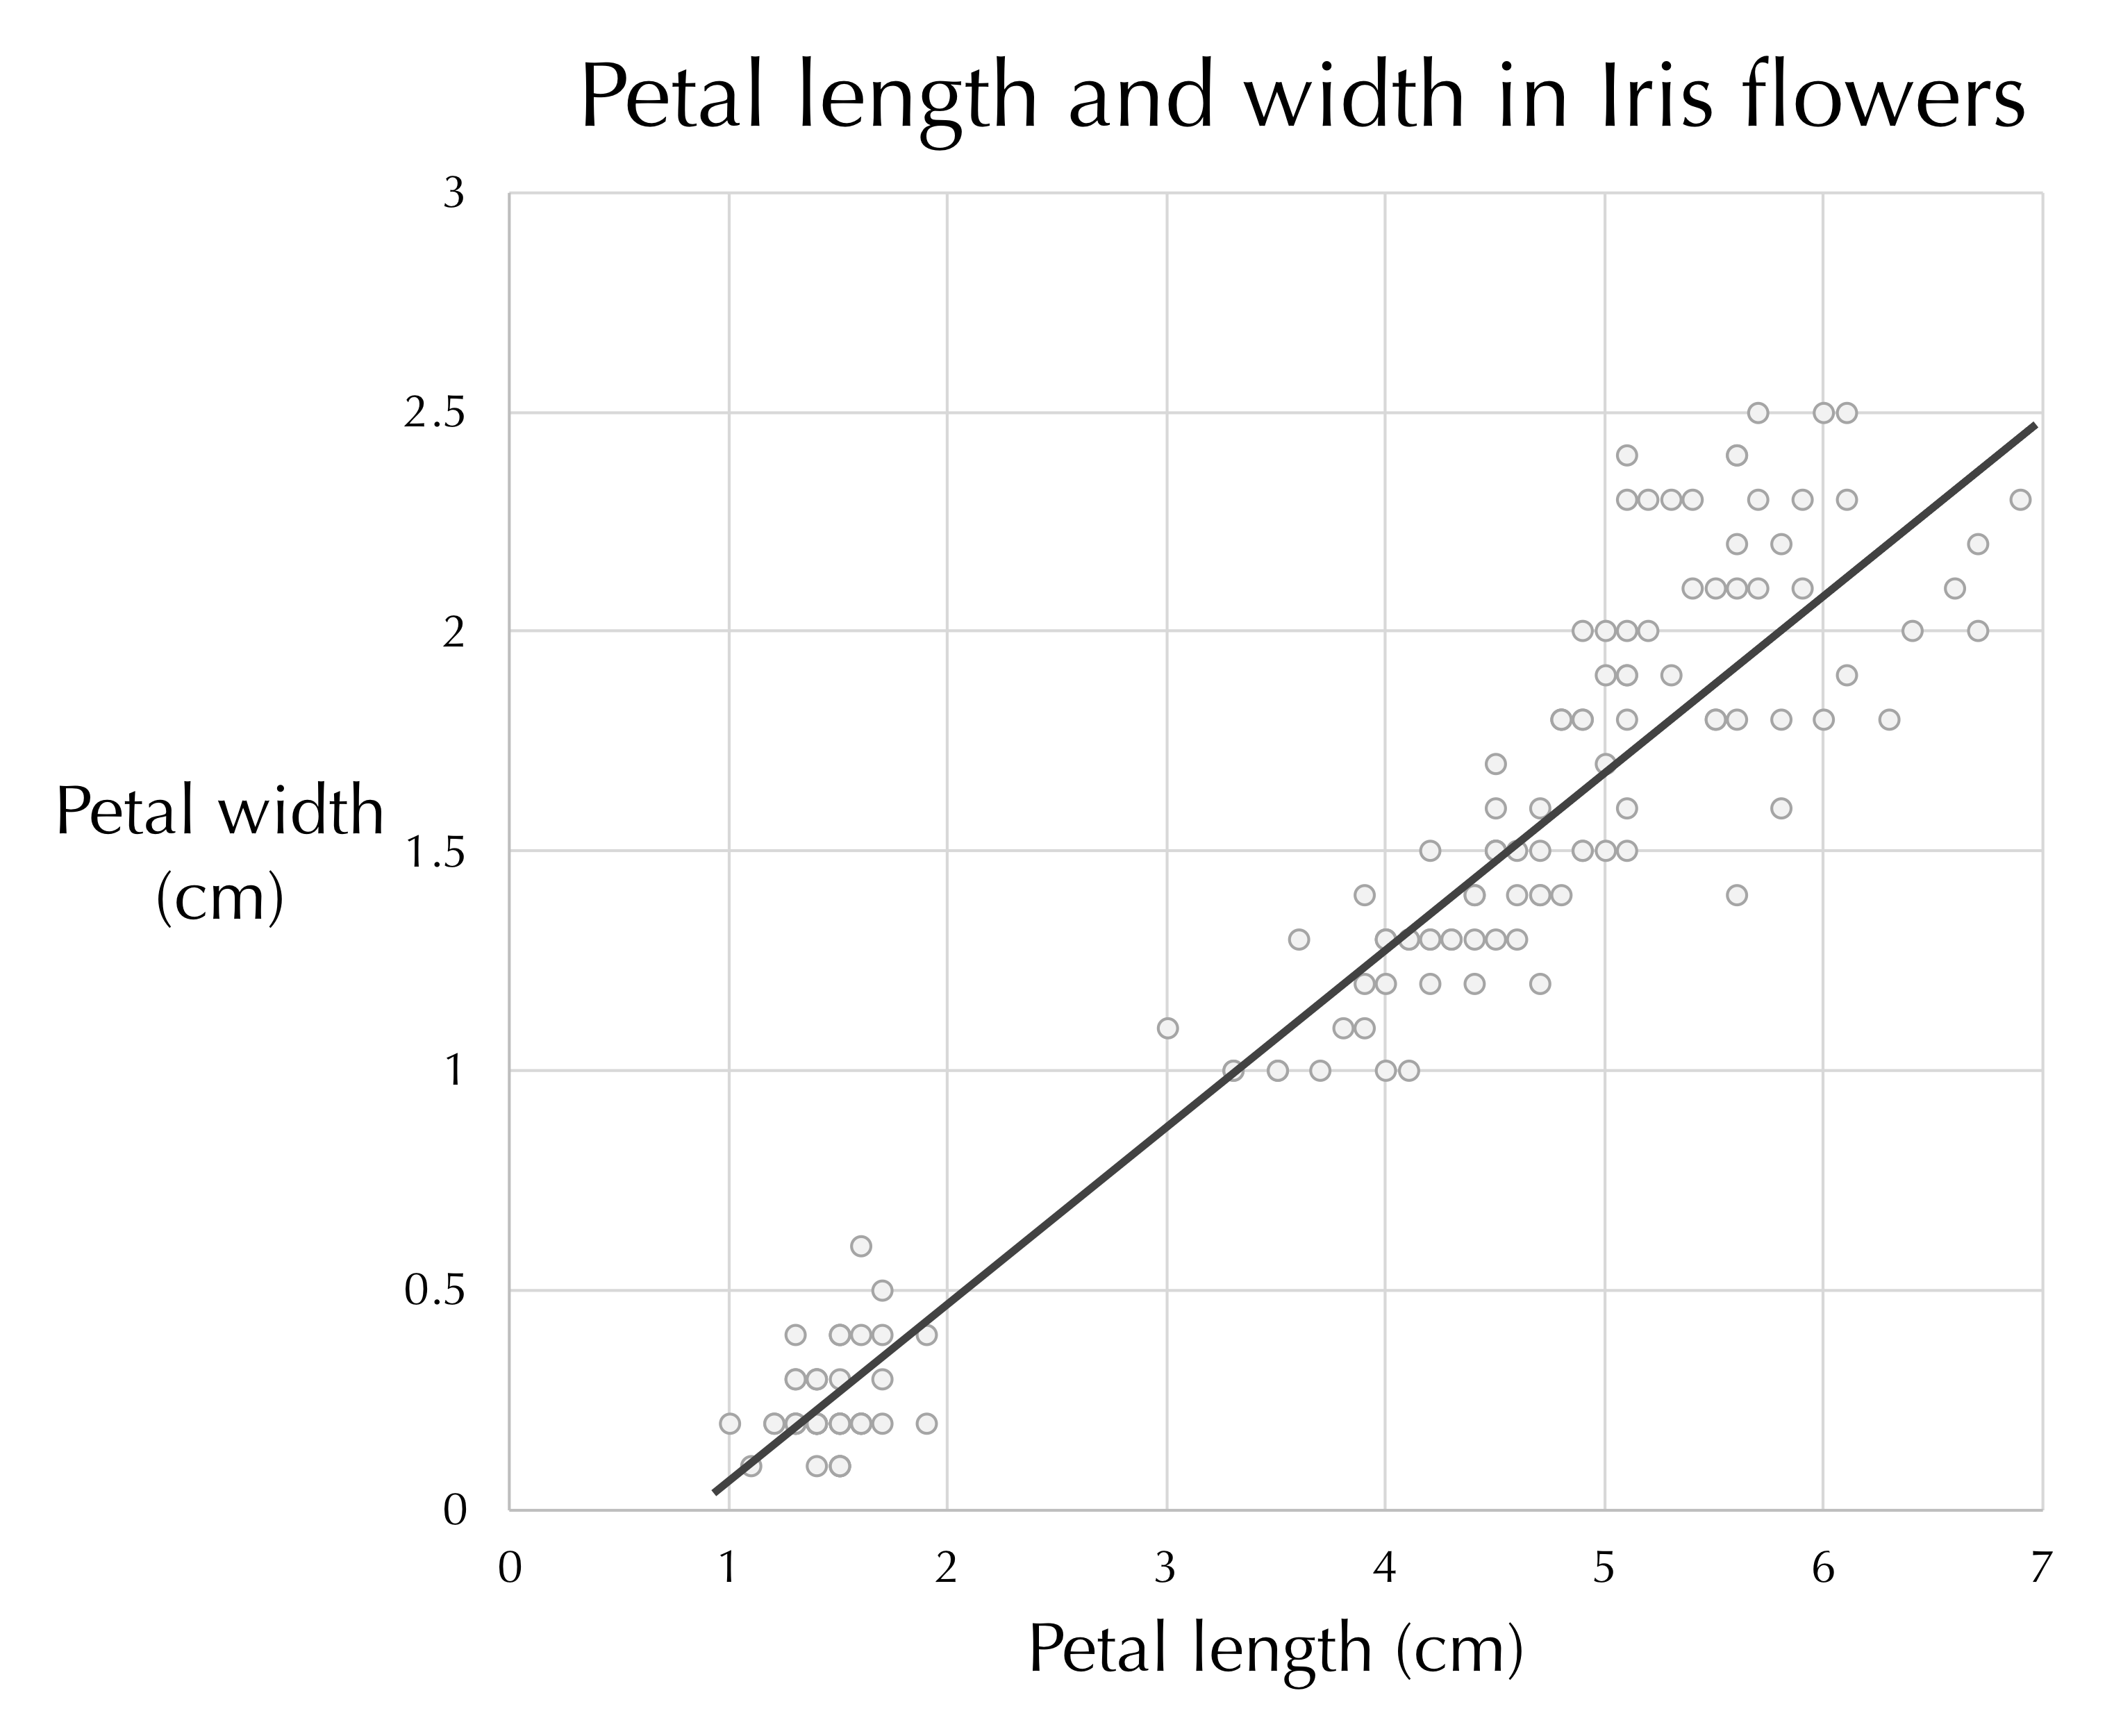
\includegraphics[width = 0.7\textwidth]{../images/iris_flowers_regression_line.png}
\caption{A line passing through the plot of iris petal length against petal width. The line tells us approximately how wide we can expect an iris petal to be given the petal's width, and vice-versa.}
\label{fig:iris_flowers_regression_line}
\end{figure}

\begin{qbox}[%
How could we have determined the line in \autoref{fig:iris_flowers_regression_line}?
]\end{qbox}

Long ago in math class, you may have learned how to choose a line to best approximate a two-dimensional dataset using \textdefnogloss{linear regression}, which we will now briefly describe. In linear regression, we first establish one variable as the \textit{dependent} variable, which is typically plotted on the y-axis. In our iris flower example, the dependent variable is petal width.

Given a line, we use $L(x)$ to denote the y-coordinate of the point on the line corresponding to a given x-coordinate. For this line, we can then define the \textdefnogloss{residual} of a data point $(x, y)$ as the difference $y - L(x)$ between its y-coordinate and the y-coordinate that the line estimates as corresponding to \textvar{x}. If a residual is positive, then the data point lies ``above'' the line, and if the residual is negative, then the point lies ``below'' the line (\autoref{fig:residuals_y_coordinates}).\\

\begin{figure}[h]
\centering
\mySfFamily
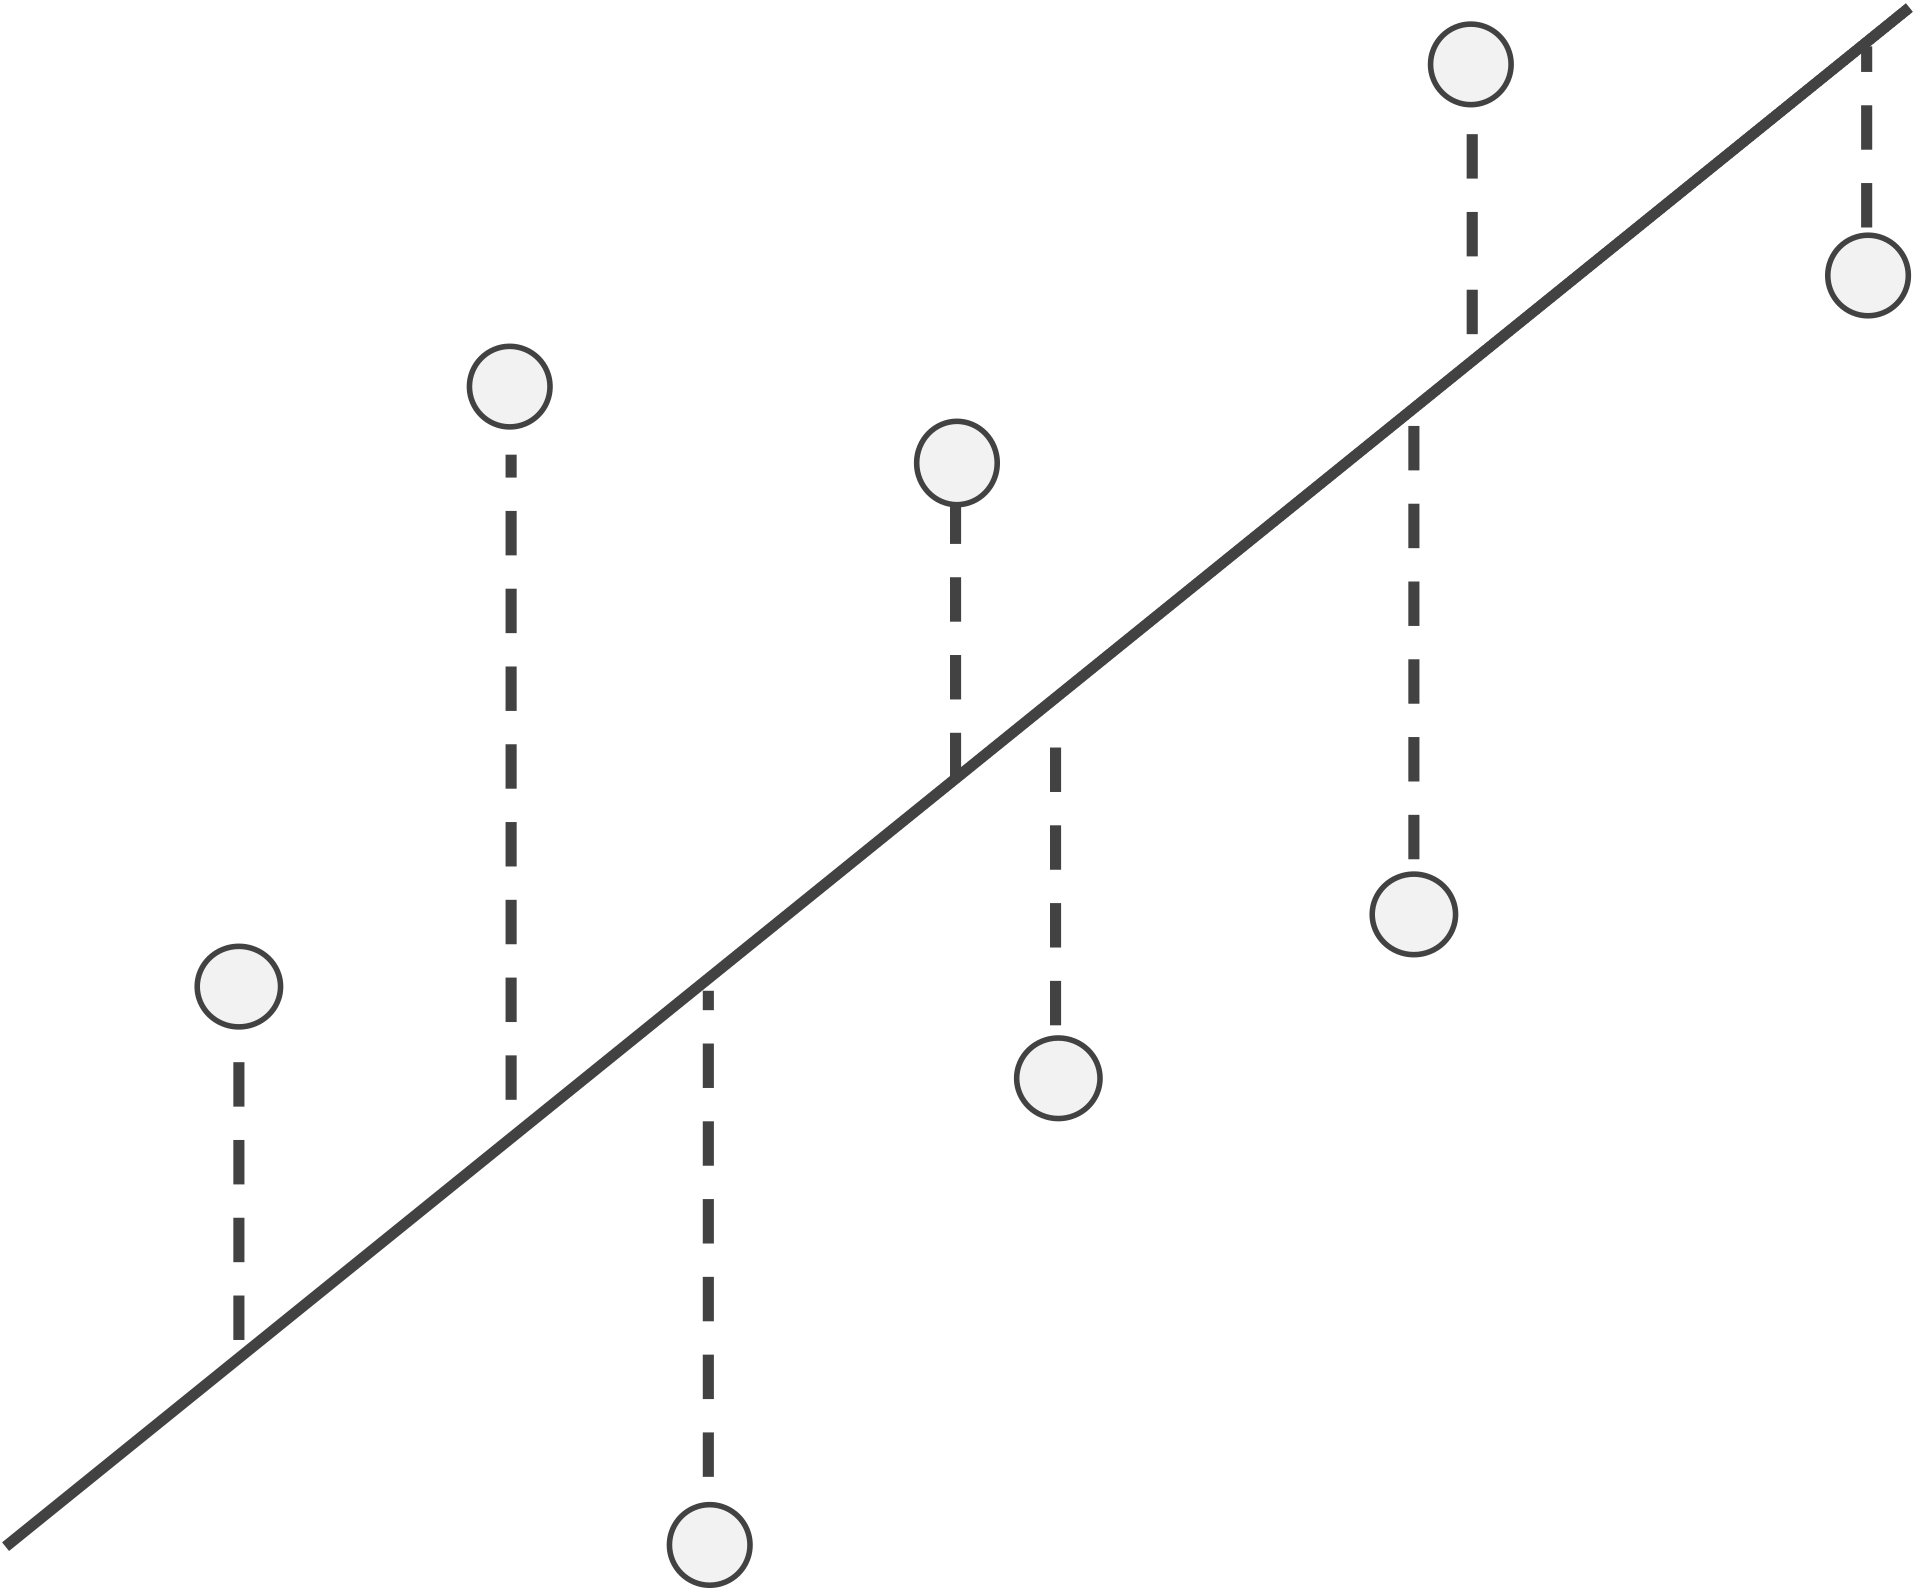
\includegraphics[width = 0.5\textwidth]{../images/residuals_y_coordinates.png}
\caption{An example line and data points with a visual depiction of the points' residuals. The absolute value of a residual is the length of its dashed line, and the sign of a residual corresponds to whether it lies above or below the line.}
\label{fig:residuals_y_coordinates}
\end{figure}

As the line changes, so will the points' residuals. The smaller the residuals become, the better the line fits the points. In linear regression, we are looking for the line that minimizes the sum of squared residuals.

Linear regression is a common approach, but it is not the only way to fit a line to a collection of data. Choosing petal width as the dependent variable makes sense if we want to explain petal width as a function of petal length, but if we were to make petal length the dependent variable instead, then linear regression would minimize the sum of squared residuals in the x-direction (\autoref{fig:residuals_x_coordinates}).\\

\begin{figure}[h]
\centering
\mySfFamily
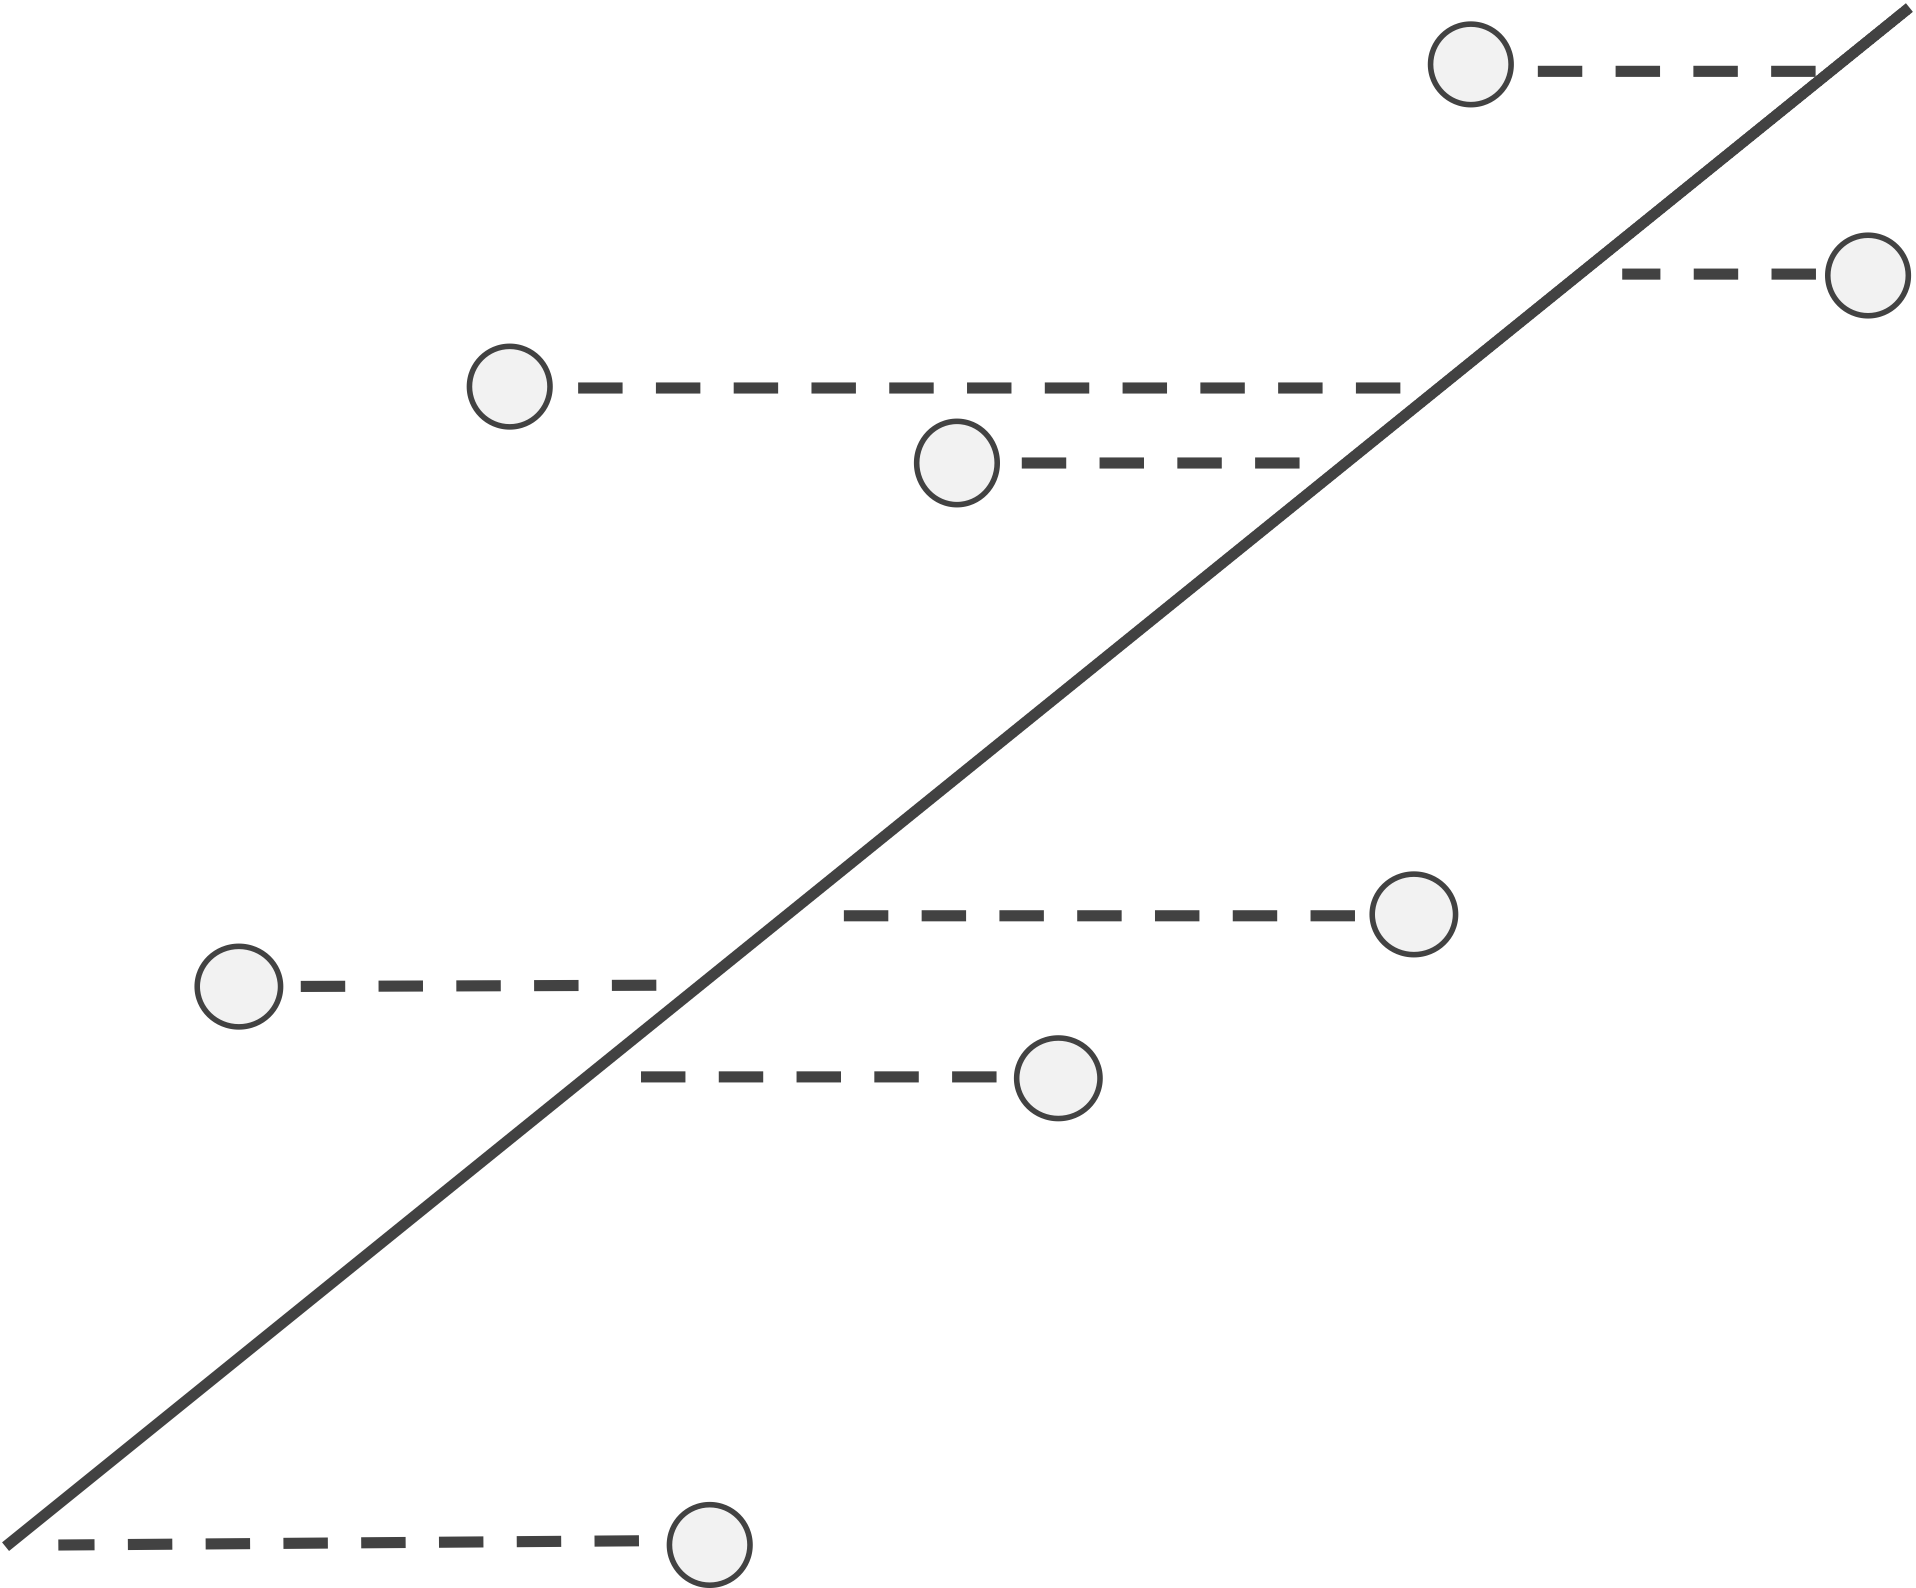
\includegraphics[width = 0.5\textwidth]{../images/residuals_x_coordinates.png}
\caption{If \textvar{x} is the dependent variable, then the residuals with respect to a line become the horizontal distances between data points and the line, and linear regression finds the line that minimizes the sum of the squares of these horizontal residuals over all possible lines through the data.}
\label{fig:residuals_x_coordinates}
\end{figure}

\begin{note}[%
The linear regression line will likely differ according to which variable we choose as the dependent variable, since the quantity that we are minimizing changes. However, if a linear pattern is present in our data, then the two regression lines will be similar.
]\end{note}

\fudgespace

\begin{qbox}[%
For the iris flower dataset, which of the two choices for dependent variable do you think is better?
]\end{qbox}

The preceding question is implying that no clear \textit{causality} underlies the correlation between petal width and petal length, which makes it difficult to prioritize one variable over the other as the dependent variable. For this reason, we will revisit how we are defining the line that best fits the data.

Instead of considering residuals based on distances to the line in only the x-direction or the y-direction, we can treat both variables equally. To do so, we examine the distance from each data point to its nearest point on the line (\autoref{fig:residuals_projections}), which is called the \textdefnogloss{projection} of the point onto the line. The line that minimizes the sum of the squares of distances between each point and its projection onto the line is called the \textdefnogloss{first principal component} of the data.

\begin{figure}[h]
\centering
\mySfFamily
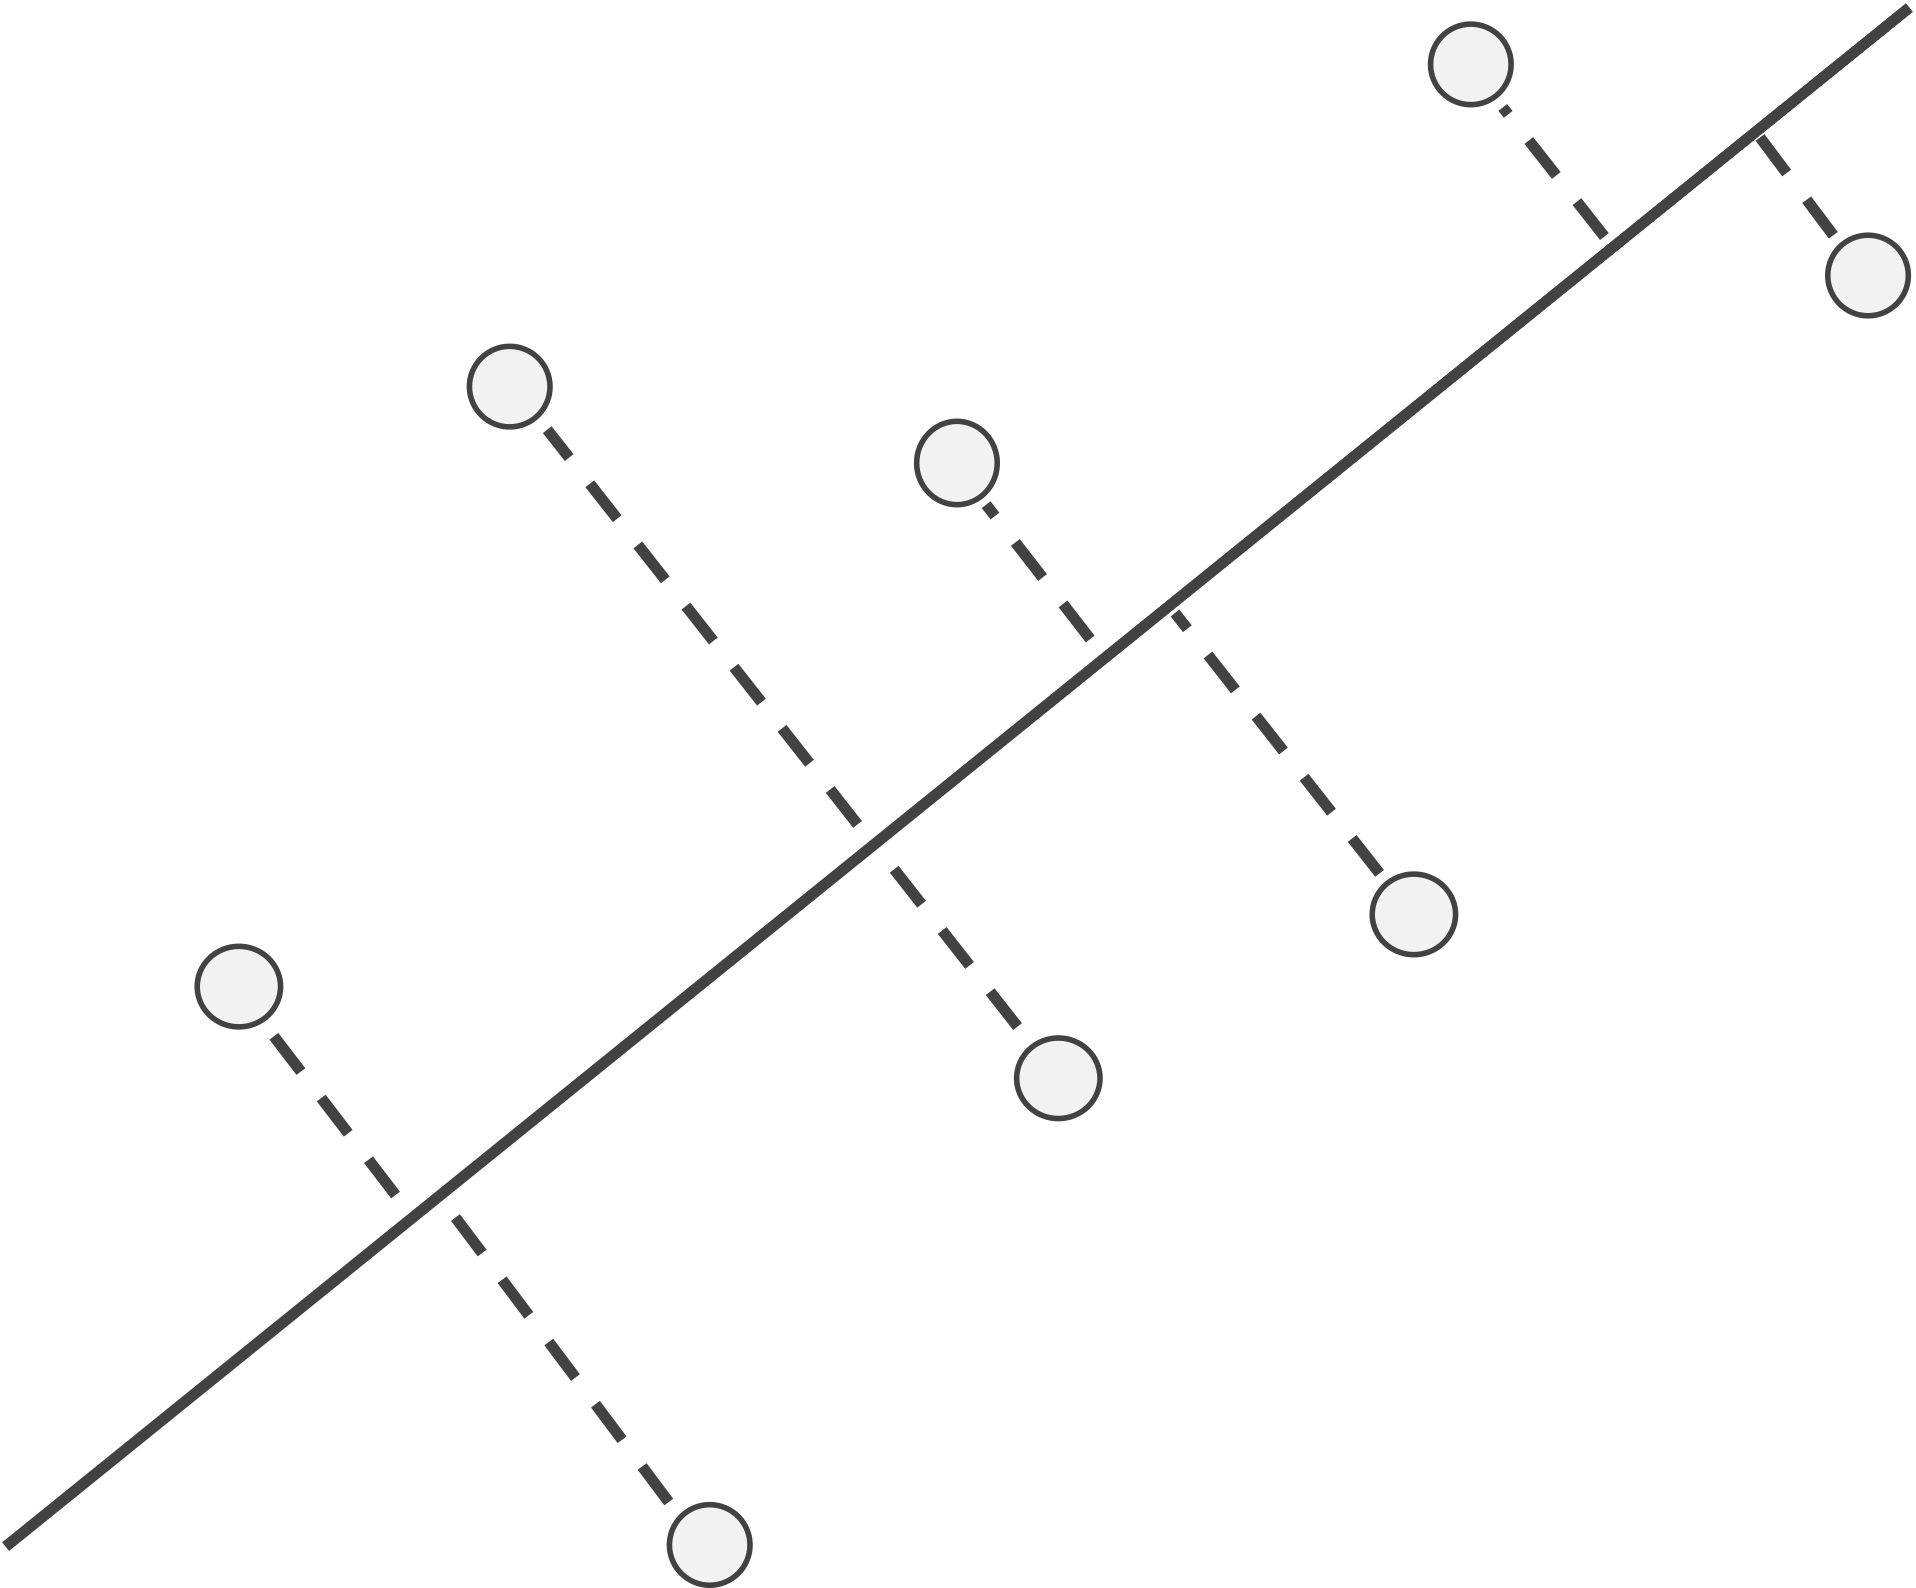
\includegraphics[width = 0.5\textwidth]{../images/residuals_projections.png}
\caption{A line along with a collection of data points; dashed lines show the shortest segments connecting each data point to its projection onto the line, which is the point on the line that is as close as possible to the data point.}
\label{fig:residuals_projections}
\end{figure}

The first principal component is often said to be the line that ``explains the most variance in the data''. If there is indeed a correspondence between lily petal width and length, then the distances from each point to the first principal component correspond to variation due to randomness. By minimizing the sum of squares of these distances, we limit the amount of variation in our data that we cannot explain.

%The following animated GIF shows a line rotating through a collection of data points, with the distance from each point to the line shown in red. As the line rotates, we can see the distances from the points to the line change.
%
%[![image-center](../assets/images/600px/pca_rotating_line_first_frame.png){: .align-center}](../assets/images/pca_rotating_line.gif)
%An animated GIF showing that the distances from points to their projections onto a line change as the line rotates. The line of best fit is the one in which the sum of the square of these distances is minimized.  Source: amoeba, StackExchange user.[^amoeba]
%{: style="font-size: medium;"}

Another benefit of finding the first principal component of a dataset is that it allows us to \textit{reduce} the dimensionality of our dataset from two dimensions to one. As a result, the projections of a collection of data points onto their first principal component gives a one-dimensional representation of the data.

Say that we wanted to generalize the ideas above to three-dimensional space. The first principal component would offer a one-dimensional explanation of the variance in the data, but perhaps a line is insufficient to this end. The points could lie very near to a plane (a two-dimensional object), and projecting these points onto the nearest plane would effectively reduce the dataset to two dimensions (\autoref{fig:three_dimensional_pca}).

\begin{figure}[h]
\centering
\mySfFamily
\tabcolsep = 1em
\begin{tabular}{m{0.4\textwidth} m{0.4\textwidth}}
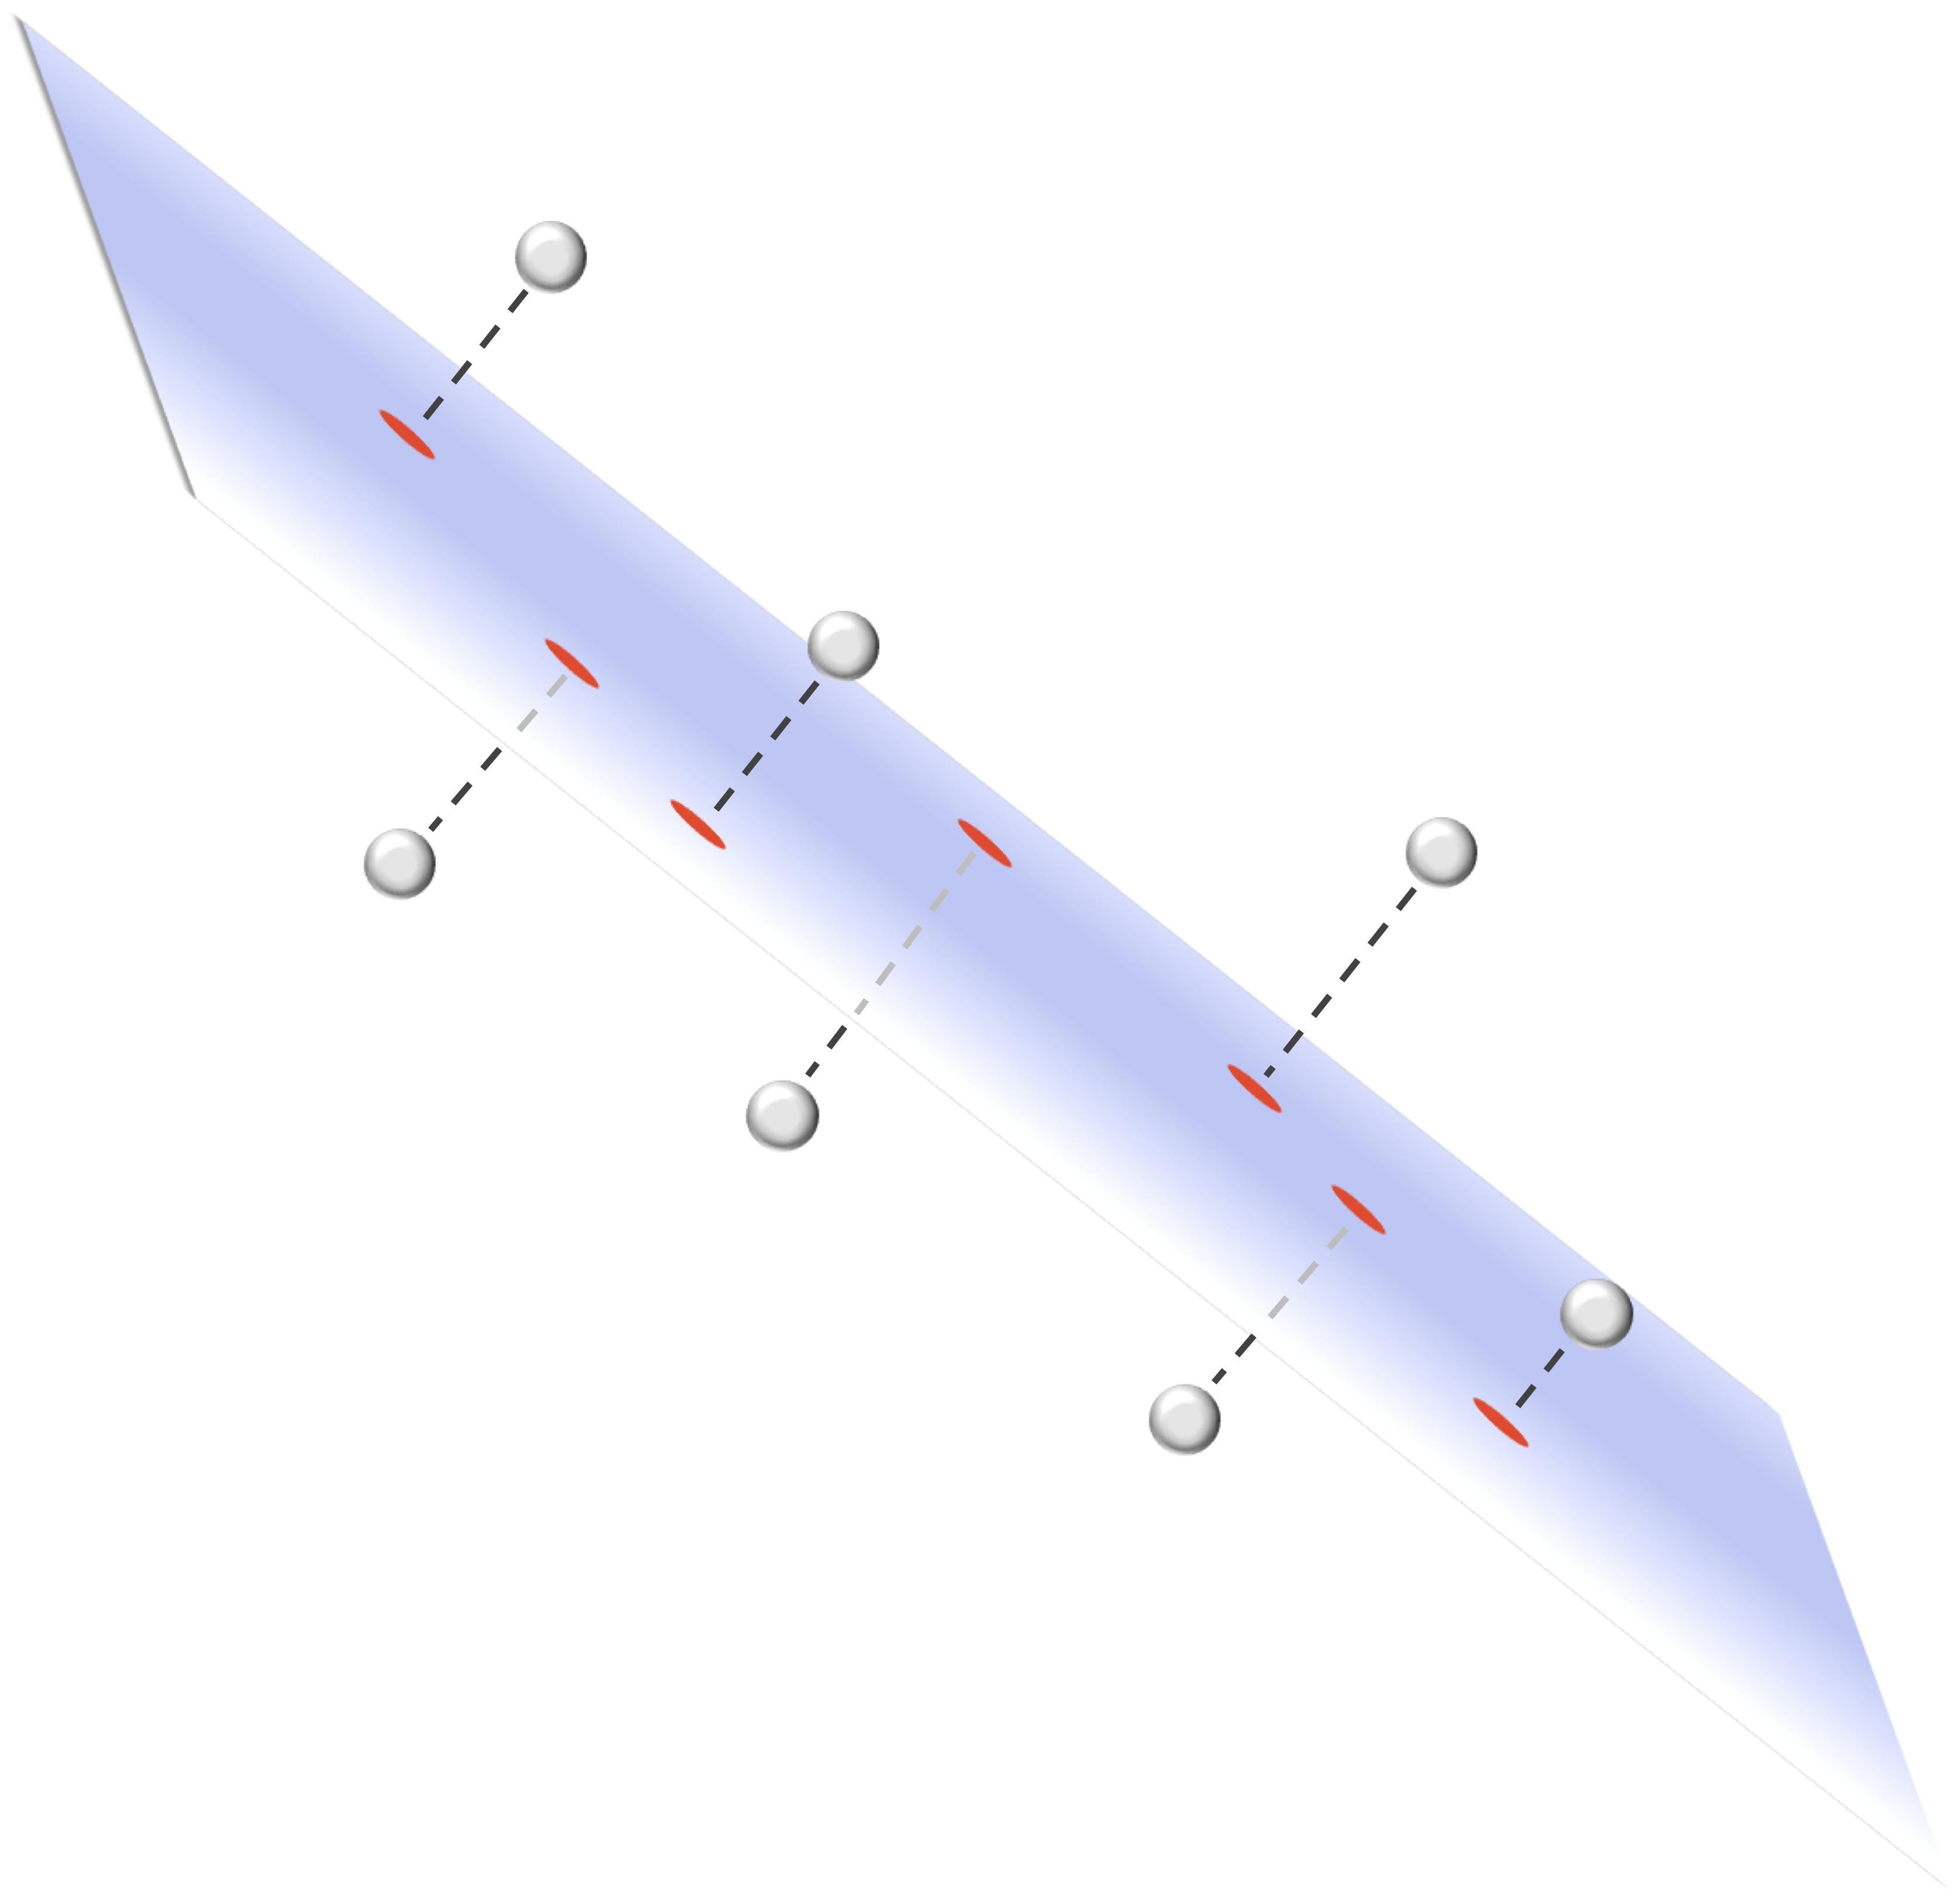
\includegraphics[width = 0.4\textwidth]{../images/three_dimensional_pca.png} &
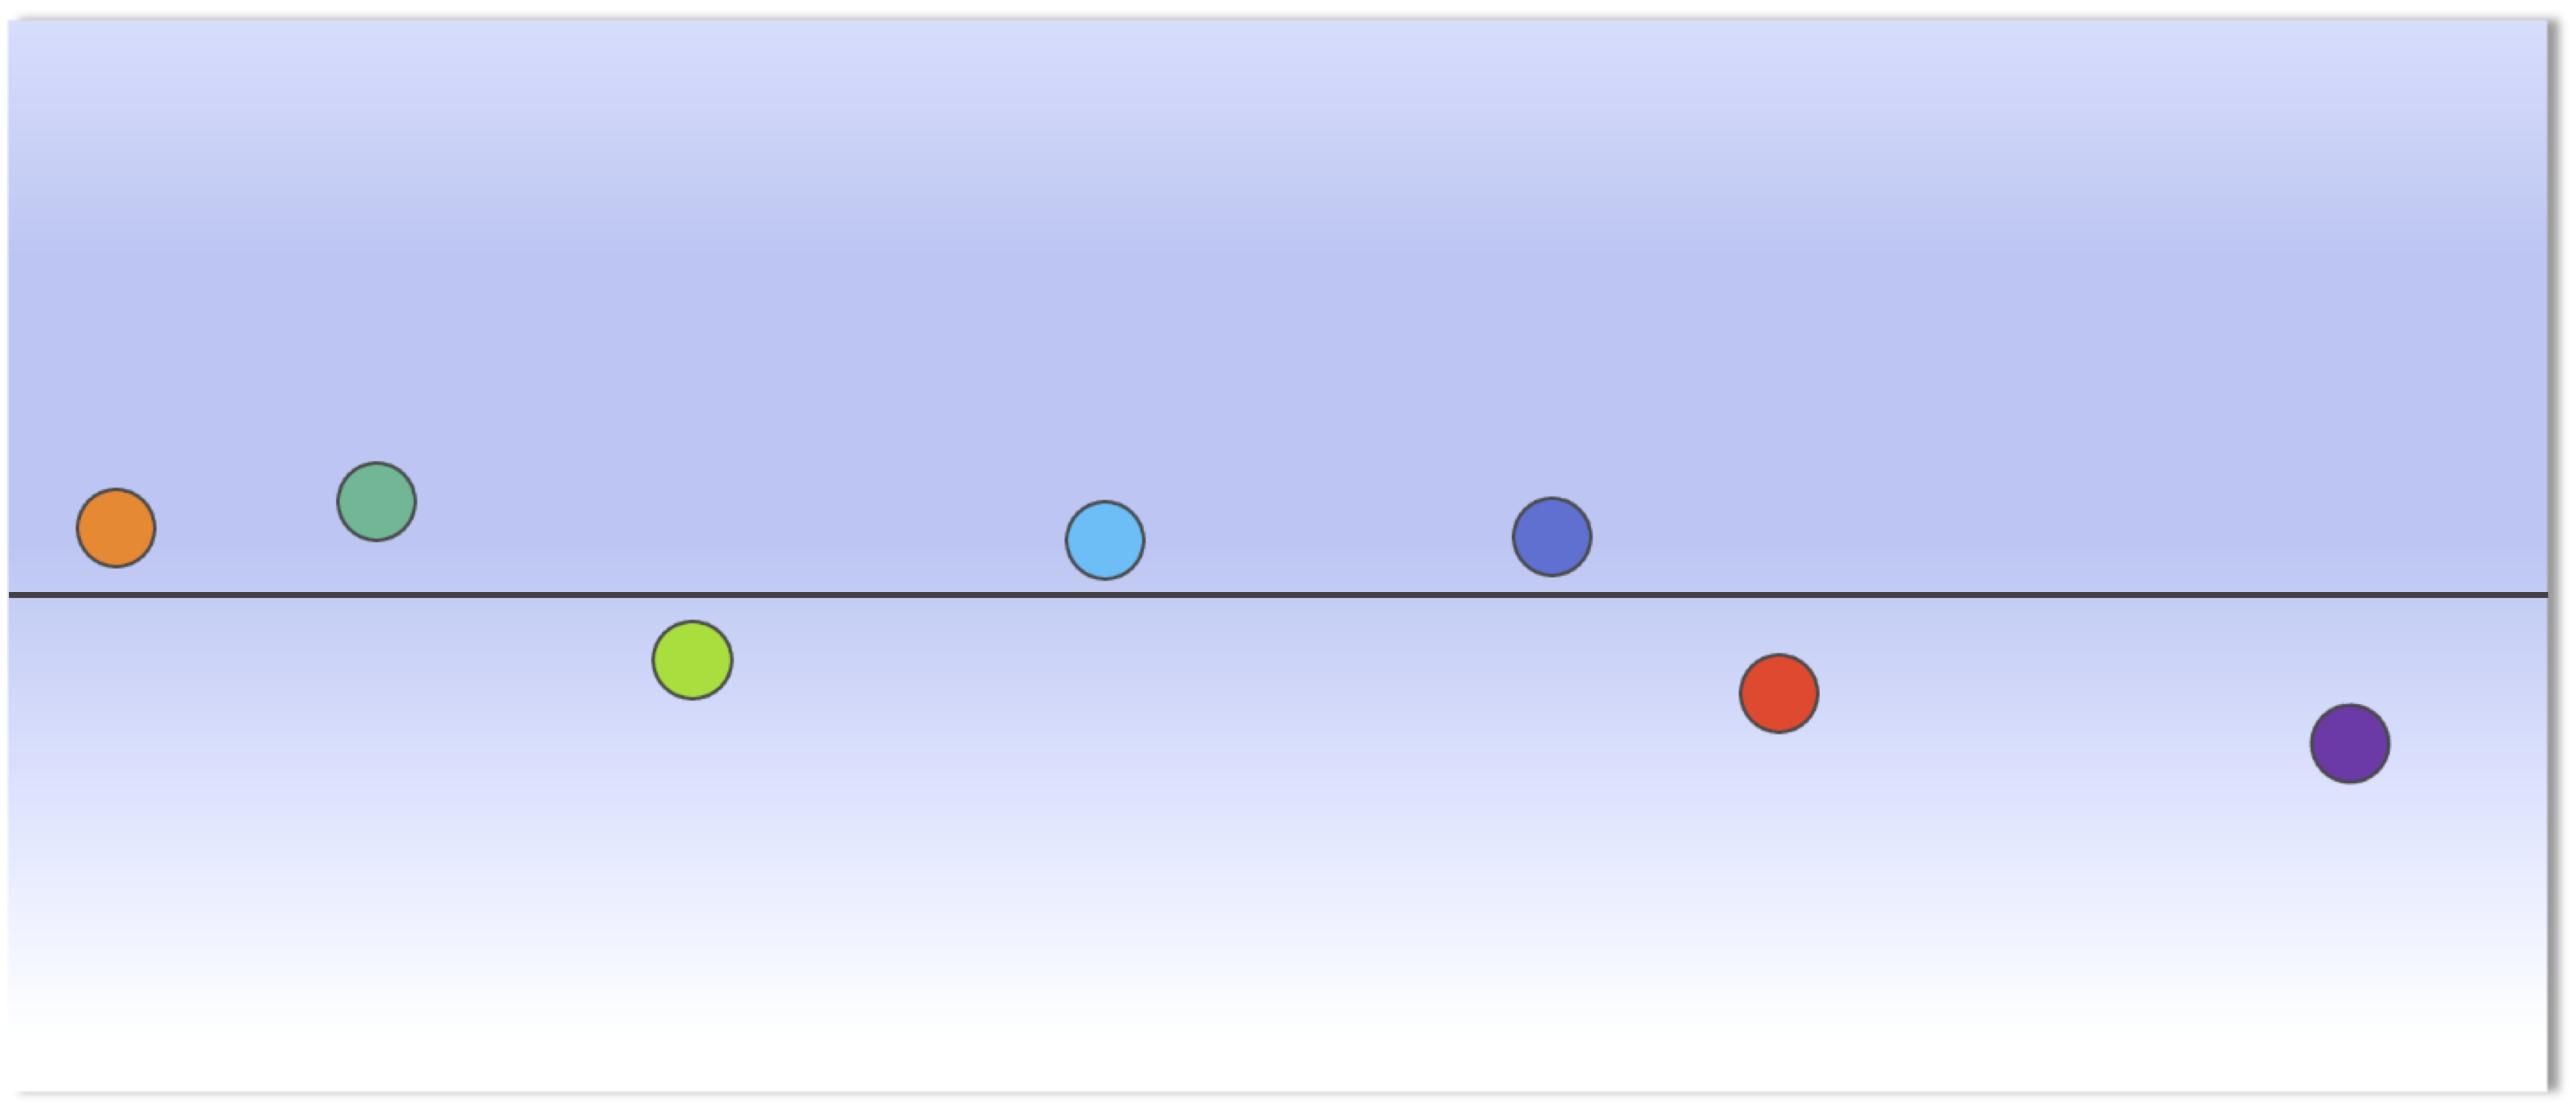
\includegraphics[width = 0.4\textwidth]{../images/three_dimensional_pca_plane.png}
\end{tabular}
\caption{(Left) A collection of seven points, each labeled with a different color. Each point is projected onto the plane that minimizes the sum of squared distances between points and the plane. The line indicated is the first principal component of the data; this line lies within the plane, which is the case for any dataset. The y-axis of this plane is the ``second principal component'' of the data. (Right) A reorientation of the plane such that the first principal component is shown as the x-axis, with colored points corresponding to the projections onto the plane from the first figure.}
\label{fig:three_dimensional_pca}
\end{figure}

Our three-dimensional minds will not permit us the intuition needed to visualize the extension of this idea into higher dimensions, but we can generalize these concepts mathematically. Given a collection of \textvar{m} data points (vectors) in \textvar{n}-dimensional space, we are looking for a \textvar{d}-dimensional \textdef{hyperplane}{hyperplane}{an embedding of \textvar{d}-dimensional space inside \textvar{n}-dimensional space}, or an embedding of \textvar{d}-dimensional space inside \textvar{n}-dimensional space, such that the sum of squared distances from the points to the hyperplane is minimized. By taking the projections of points to their nearest point on this hyperplane, we reduce the dimension of the dataset from \textvar{n} to \textvar{d}. This approach, which is over 100 years old but omnipresent in modern data science, is called \textdef{principal component analysis (PCA)}{principal component analysis (PCA)}{an approach used for finding the lower-dimensional hyperplane through a collection of data minimizing the distances from the points to the hyperplane}.\\

\begin{note}[%
It can be proven that for any dataset, when $d_1$ is smaller than $d_2$, the hyperplane provided by PCA of dimension $d_1$ is \textit{always} a subset of the hyperplane of dimension $d_2$. For example, the first principal component is always found within the plane ($d = 2$) provided by PCA, which was indicated in \autoref{fig:three_dimensional_pca} (left).
]\end{note}

\FloatBarrier
\phantomsection
\subsection{Visualizing the WBC shape space after PCA}

\autoref{fig:cellorg_pca_graph} (top) shows the shape space of WBC images, reduced to three dimensions by PCA, in which each image is represented by a point that is color-coded according to its cell family. We can also subdivide granulocytes into basophils, eosinophils, and neutrophils. Updating our labels according to this subdivision produces the plot in \autoref{fig:cellorg_pca_graph} (bottom).\tutorial[white_blood_cells/tutorial_shape_space]

\begin{figure}[p]
\centering
\mySfFamily
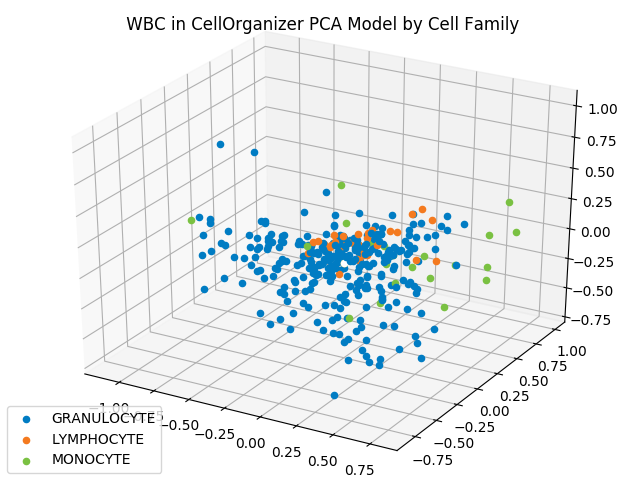
\includegraphics[width = 0.7\textwidth]{../images/cellorg_pca_graph.png}\\[4ex]
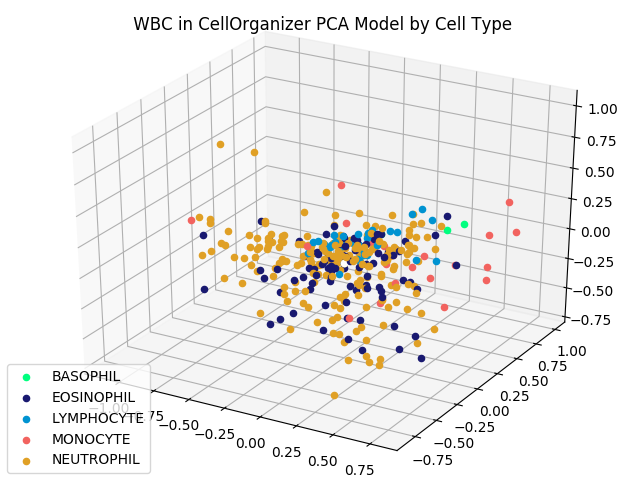
\includegraphics[width = 0.7\textwidth]{../images/cellorg_pca_graph_cell.png}
\caption{(Top) The projection of each WBC shape vector onto a three-dimensional PCA hyperplane (\textvar{d} = 3). (Bottom) The same shape space, with granulocytes subdivided into basophils, eosinophils, and neutrophils.}
\label{fig:cellorg_pca_graph}
\end{figure}



Although images from the same family do not cluster as tightly as the iris flower dataset --- which could be criticized as an unrealistic representation of real datasets --- images from the same type do appear to be nearby. This fact should give us hope that proximity in a shape space of lower dimension may help us correctly classify images of unknown type.\\

\FloatBarrier
\phantomsection

\section{Classifying White Blood Cell Images}
\label{sec:training}

\phantomsection
\subsection{Cross validation}

We would like to apply k-NN to a dimension-reduced shape space WBC images to see how often it assigns an image to the correct class. However, we already know the correct class for every image in our dataset! 

One approach for assessing how well a classification algorithm performs when the classes of each object in our dataset are known is to exclude some \textit{subset} of the data, called the \textdefnogloss{validation set}. After hiding the correct classes for elements of the validation set from the classification algorithm, we will measure how often the algorithm correctly identifies the class of each object in this set.

Yet it remains unclear which subset of the data we should use as a validation set. Random variation could cause that the classifier's accuracy will change depending on which subset we choose. After all, what makes the elements of the validation set so special as to be chosen? Ideally, we would use a more democratic approach that is not subject to random variation and that uses \textit{all} of the data for validation.

In \textdef{cross validation}{cross validation}{an approach used in classification (or other machine learning approaches) in which we divide the data into approximately equally sized groups called folds; over multiple rounds, one fold is used as a validation set, pretending that we do not know the correct class of these data points, and we then determine how well the algorithm performs at identifying the correct class of each point}, we divide our data into a collection of \textvar{f} (approximately) equally sized groups called \textdefnogloss{folds}. We use one of these folds as a validation set, keeping track of which objects the classification algorithm classifies correctly, and then we start over with a different fold as our validation set. In this way, every element in our dataset will get used as a member of a validation set exactly once.

\FloatBarrier
\phantomsection
\subsection{A first attempt at quantifying the success of a classifier}

Before applying cross validation to WBC images, we will discuss how to quantify the performance of a classifier. \autoref{fig:iris_confusion_matrix} shows the result of applying k-NN to the iris flower dataset, using \textvar{k} equal to 3 and cross validation with \textvar{f} equal to 10 (since there are 150 flowers, each fold contains 15 flowers). This table is called a \textdef{confusion matrix}{confusion matrix}{a table used to measure the results of a classification algorithm, identifying how many items from each known class were assigned to each class by the algorithm} because it visualizes whether an algorithm is ``confusing'' an object's class assignment.

\begin{figure}[h]
\centering
\tabcolsep = 1 em
\mySfFamily
\rowcolors{2}{gray!25}{white}
\begin{tabular}{r c c c}
%\rowcolor{gray!50}
%& \multicolumn{3}{c}{\textbf{Predicted class}}\\
\rowcolor{gray!50}
& \textbf{\textit{I.~setosa}} & \textbf{\textit{I.~versicolor}} & \textbf{\textit{I.~virginica}} \\
\textbf{\textit{I.~setosa}} & 50 & \phantom{5}0 & \phantom{5}0 \\
\textbf{\textit{I.~versicolor}} & \phantom{5}0 & 47 & \phantom{5}3 \\
\textbf{\textit{I.~virginica}} & \phantom{5}0 & \phantom{5}4 & 46
\end{tabular}
\caption{The confusion matrix resulting from applying k-NN to the iris flower dataset, using $\textvar{k} = \text{1}$ and cross validation with $\textvar{f} = \text{10}$.}
\label{fig:iris_confusion_matrix}
\end{figure}

In a confusion matrix, rows correspond to true classes, and columns correspond to predicted classes. For example, consider the second row in \autoref{fig:iris_confusion_matrix}, which corresponds to the flowers that we know are \textit{Iris versicolor}. k-NN predicted that none of these flowers were \textit{Iris setosa}, that 47 of these flowers were \textit{Iris versicolor}, and that three of the flowers were \textit{Iris virginica}. Therefore, it correctly predicted the class of 47 of the 50 total \textit{Iris versicolor} flowers.\\

\begin{note}[%
We did not apply dimension reduction to the iris flower dataset because it has only four dimensions.
]\end{note}

We define the \textdef{accuracy}{accuracy}{the fraction of data points that a classification algorithm correctly classifies out of the total number of data points} of a classifier as the fraction of objects that it correctly identifies out of the total. For the above iris flower example, the confusion matrix indicates that k-NN has an accuracy of $(50 + 47 + 46)/150 = 95.3\%$.

It may seem that accuracy is the only metric that we need. But if we were in a smarmy mood, then we might design a classifier for our WBC dataset that produces the confusion matrix in \autoref{fig:wbc_clown_matrix}.\\

\begin{figure}[h]
\centering
\tabcolsep = 1 em
\mySfFamily
\rowcolors{2}{gray!25}{white}
\begin{tabular}{r c c c}
\rowcolor{gray!50}
& \textbf{Granulocyte} & \textbf{Monocyte} & \textbf{Lymphocyte} \\
\textbf{Granulocyte} & 291 & 0 & 0 \\
\textbf{Monocyte} & \phantom{5}21 & 0 & 0 \\
\textbf{Lymphocyte} & \phantom{5}33 & 0 & 0
\end{tabular}
\caption{The confusion matrix for our WBC image dataset produced by classifying every image as a granulocyte.}
\label{fig:wbc_clown_matrix}
\end{figure}

\begin{qbox}[%
What is the accuracy of this classifier?
]\end{qbox}

Our clown classifier blindly assigned every image in the dataset to be a granulocyte, but its accuracy is $291/345 = 84.3\%$! To make matters worse, \autoref{fig:wbc_better_confusion_matrix} shows a confusion matrix for a hypothetical classifier on the same dataset that is clearly better but that has an accuracy of only $(232 + 17 + 26)/345 = 79.7\%$. The failure of this classifier to attain the same accuracy as the one assigning the majority class to each element owes to the WBC dataset having \textit{imbalanced} classes, which means that reporting only a classifier's accuracy may be misleading.\\

\begin{figure}[h]
\centering
\tabcolsep = 1 em
\mySfFamily
\rowcolors{2}{gray!25}{white}
\begin{tabular}{r c c c}
\rowcolor{gray!50}
& \textbf{Granulocyte} & \textbf{Monocyte} & \textbf{Lymphocyte} \\
 \textbf{Granulocyte} & 232 & 25 & 34 \\
\textbf{Monocyte} & \phantom{55}2 & 17 & \phantom{5}2 \\
\textbf{Lymphocyte} & \phantom{55}6 & \phantom{5}1 & 26
\end{tabular}
\caption{A hypothetical confusion matrix for our WBC image dataset.}
\label{fig:wbc_better_confusion_matrix}
\end{figure}

For another example, say that we design a sham medical test for some condition that always comes back negative. If 1\% of the population at a given point in time is positive for the condition, then we could report that our test is 99\% accurate. But we would fail to get this test approved for widespread use because it never correctly identifies an individual who has the condition.\\

\begin{qbox}[%
What other metrics could we design for measuring the success of a classifier?
]\end{qbox}

\FloatBarrier
\phantomsection
\subsection{Recall, specificity, and precision}

To motivate our discussion of other classifier metrics, we will continue with the analogy of medical tests, which can be thought of as classifiers with two classes (positive or negative).

First, we define some terms. A \textdef{true positive}{true positive}{a positive test in an individual who is positive for the condition} is a positive test in a patient that has the condition; a \textdef{false positive}{false positive}{a positive test in an individual who is negative for the condition} is a positive test in a patient that does not have the condition; a \textdef{true negative}{true negative}{a negative test in an individual who is negative for the condition} is a negative test in a patient that does not have the condition; and a \textdef{false negative}{false negative}{a negative test in an individual who is positive for the condition} is a negative test in a patient that does have the condition. \autoref{fig:medical_test_confusion_matrix} shows the locations of these four terms in the two-class confusion matrix for the test.\\

\begin{figure}[h]
\centering
\mySfFamily
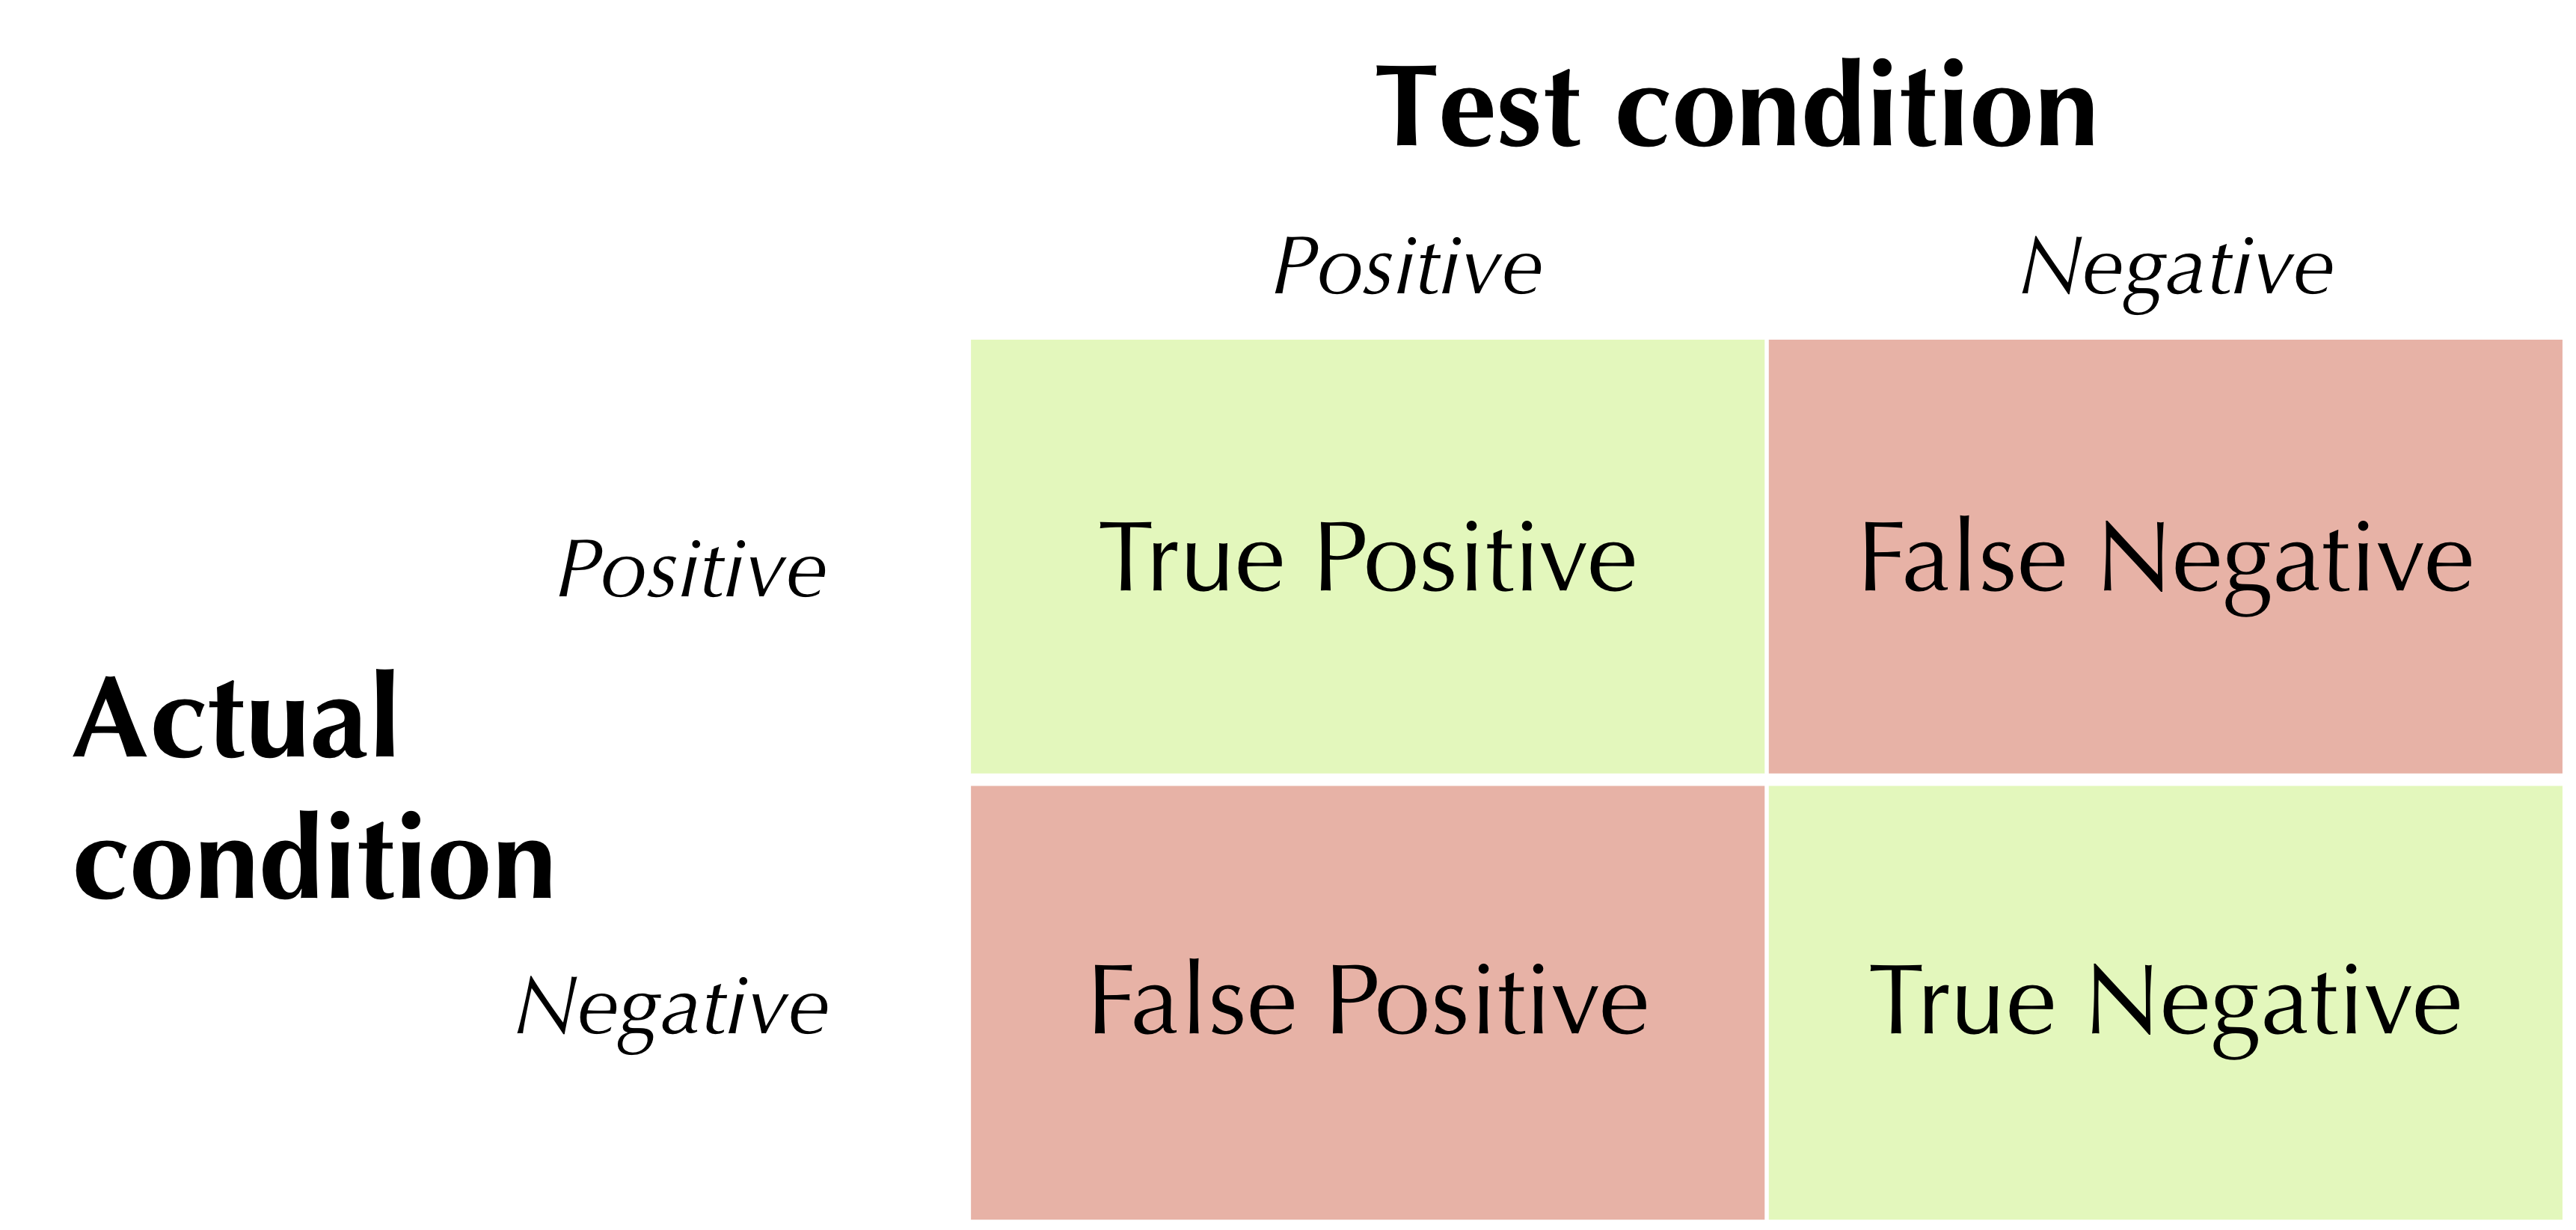
\includegraphics[width = 0.7\textwidth]{../images/medical_test_confusion_matrix.png}
\caption{The locations of true positives, true positives, true negatives, and false negatives in the confusion matrix associated with a medical test. Correct predictions are shown in green, and incorrect predictions are shown in red.}
\label{fig:medical_test_confusion_matrix}
\end{figure}

In what follows, we will work with the confusion matrix for a hypothetical medical test shown in \autoref{fig:medical_test_confusion_matrix_hypothetical}. Note that this test has lower accuracy than our sham test that returns negative for all individuals, but we will now show metrics for which it is superior.\\

\begin{figure}[h]
\centering
\tabcolsep = 1 em
\mySfFamily
\rowcolors{2}{gray!25}{white}
\begin{tabular}{r c c}
\rowcolor{gray!50}
& \textbf{Positive} & \textbf{Negative} \\
 \textbf{Positive} & 1,000 & \phantom{198,}500 \\
\textbf{Negative} & 2,000 & 198,000 \\
\end{tabular}
\caption{The confusion matrix for a hypothetical medical test.}
\label{fig:medical_test_confusion_matrix_hypothetical}
\end{figure}

%\begin{figure}[h]
%\centering
%\mySfFamily
%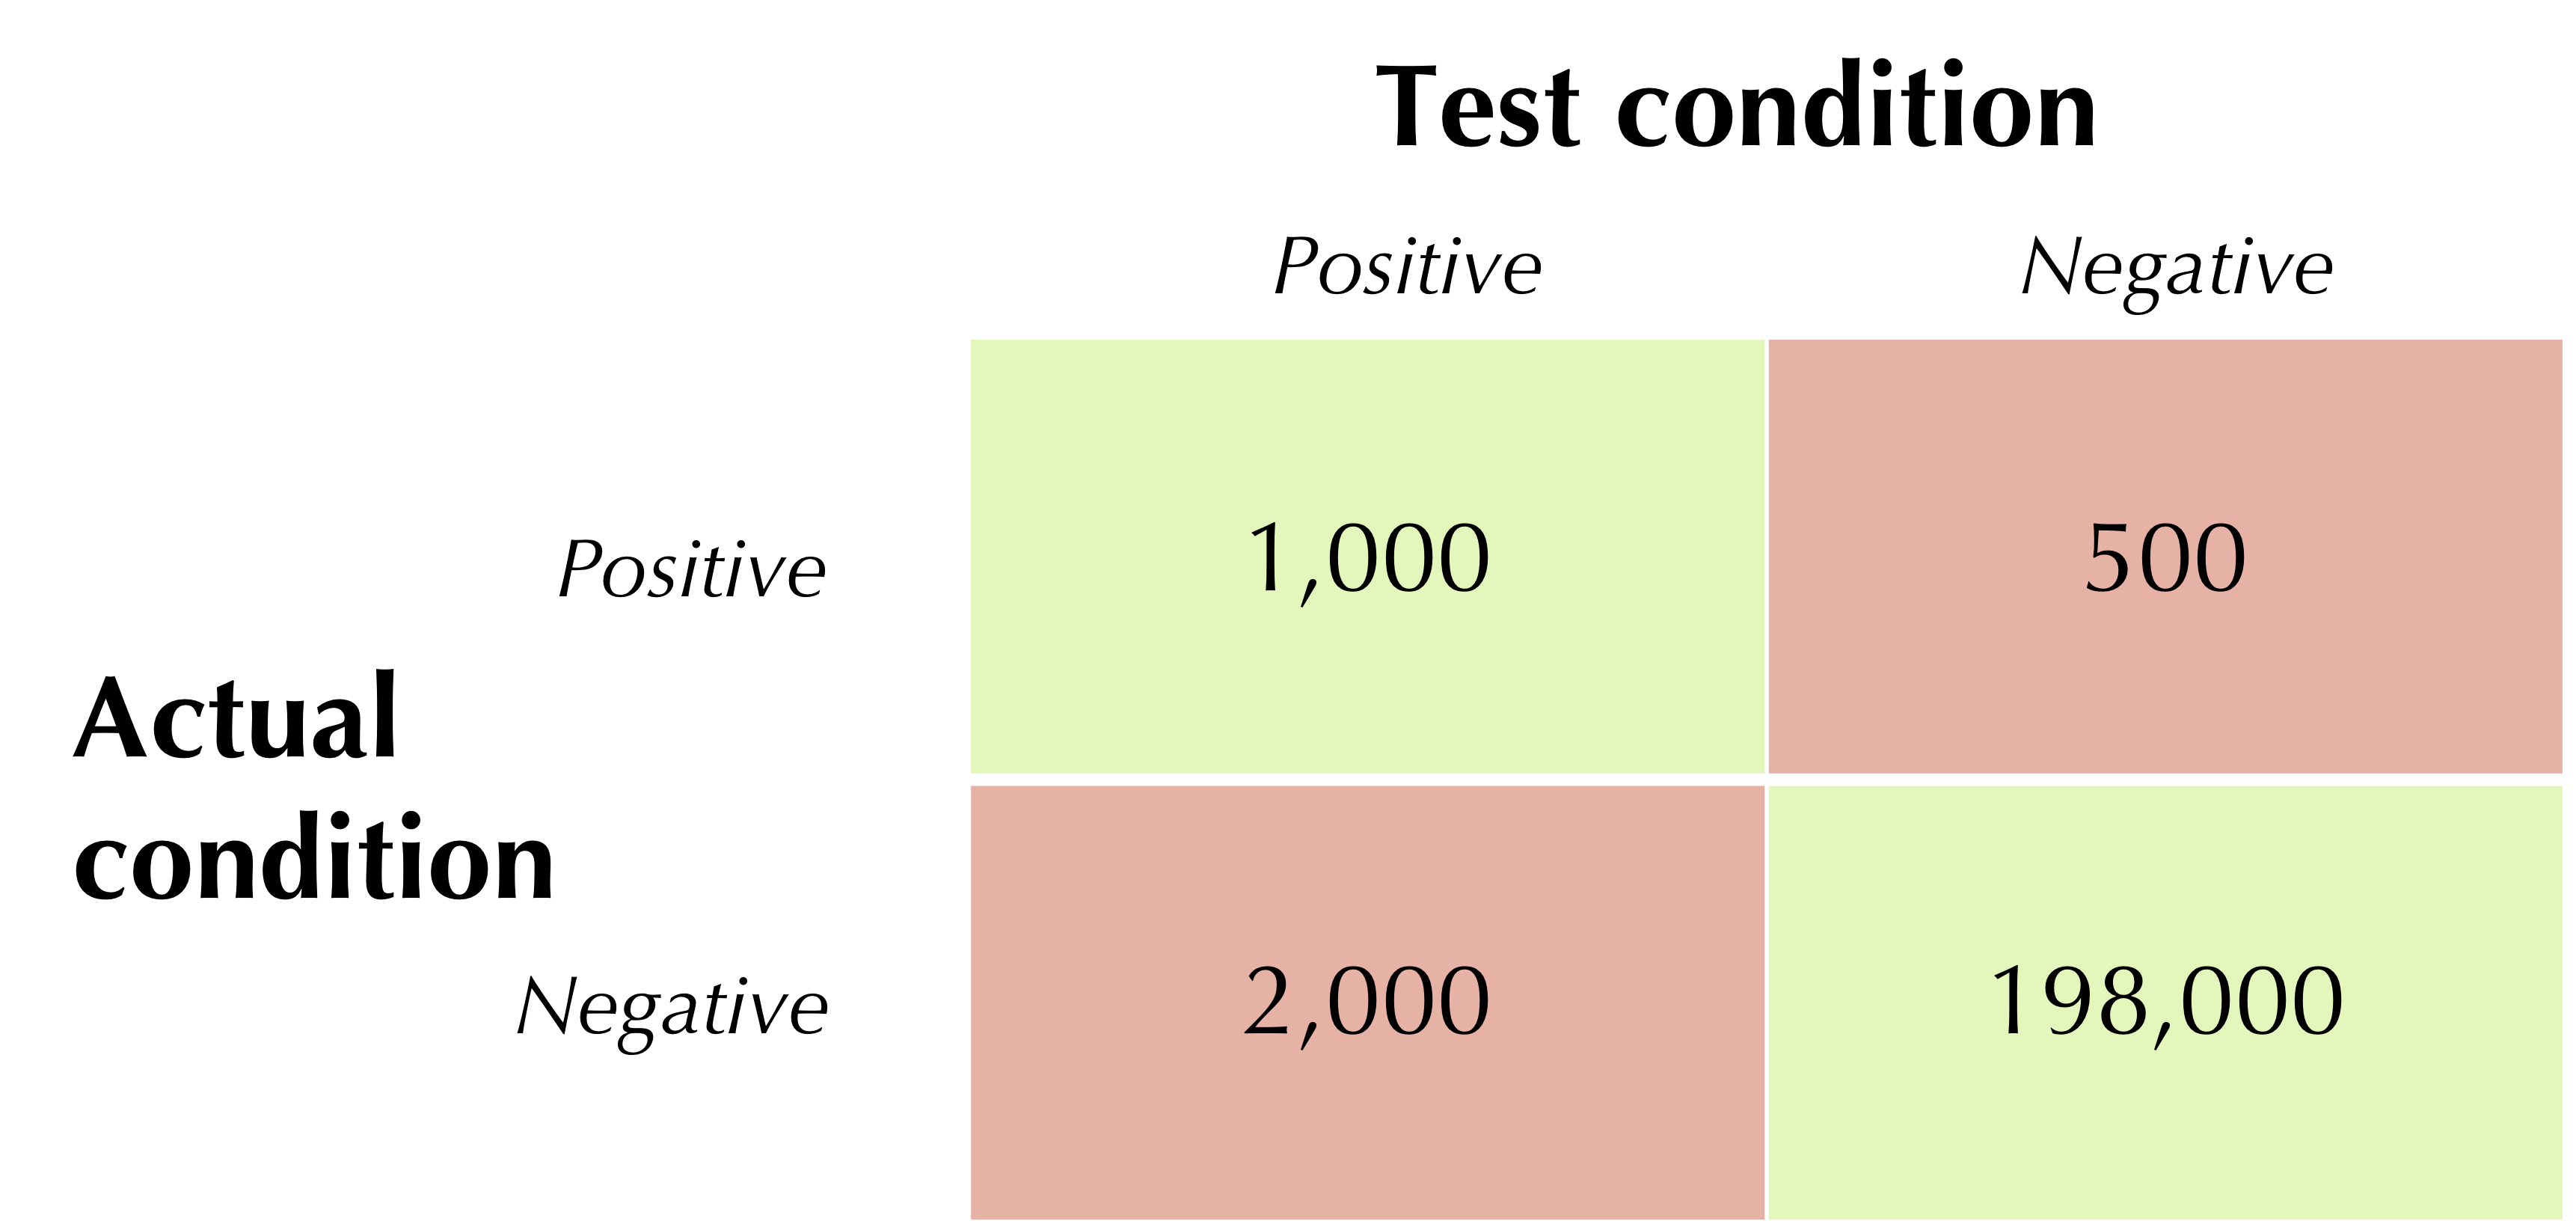
\includegraphics[width = 0.7\textwidth]{../images/medical_test_confusion_matrix_hypothetical.png}
%\caption{A hypothetical COVID test confusion matrix.}
%\label{fig:medical_test_confusion_matrix_hypothetical}
%\end{figure}

The \textdef{recall}{recall (sensitivity)}{the percentage of positive cases that a two-class classifier such as a medical test correctly identifies, or the ratio of true positives over the sum of the true positives and false negatives} (a.k.a.~\textdefnogloss{sensitivity}) of a two-class classifier is the percentage of positive cases that the test correctly identifies, or the ratio of true positives over the sum of the true positives and false negatives (found by summing the top row of the confusion matrix). For the confusion matrix in \autoref{fig:medical_test_confusion_matrix_hypothetical}, the recall is $1,000/(1,000 + 500) = 66.7\%$. Recall ranges from 0 to 1, with larger values indicating that the test is ``sensitive'', meaning that it can identify true positives from a pool of patients who actually are positive.

The \textdef{specificity}{specificity}{the ratio of true negatives to the sum of true negatives and false positives for a two-class classifier such as a medical test} of a test is an analogous metric for patients whose actual status is negative. Specificity measures the ratio of true negatives to the sum of true negatives and false positives (found by summing the second row of the confusion matrix). The test with confusion matrix in \autoref{fig:medical_test_confusion_matrix_hypothetical} has specificity equal to $198,000/(198,000 + 2,000) = 99\%$.

Finally, the \textdef{precision}{precision}{the percentage of positive tests that are correct for a two-class classifier such as a medical test, formed by taking the ratio of true positives to the sum of true positives and false positives} of a test is the percentage of positive tests that are correct, formed by taking the ratio of true positives to the total number of positive tests (found by summing the first column of the confusion matrix). For example, the test with confusion matrix in \autoref{fig:medical_test_confusion_matrix_hypothetical} has precision equal to $1,000/(1,000 + 2,000) = 33.3\%$.\\

\begin{qbox}[%
How could we trick a test to have recall, specificity, or precision close to 1?
]\end{qbox}

Just like accuracy, all three of the metrics we have just introduced are imperfect and can be fooled by frivolous tests that always return positive or negative. However, a frivolous test cannot score well on all these metrics at the same time. Therefore, in practice we will examine all these metrics, as well as accuracy, when assessing the quality of a classifier.\\

\begin{qbox}[%
Consider a dataset of 201,500 patients, 1,500 of whom have a condition. Compute the recall, specificity, and precision of a hypothetical medical test for the condition that always returns negative. How does each metric compare against those of the hypothetical test in \autoref{fig:medical_test_confusion_matrix_hypothetical}?
]\end{qbox}

You may find all these terms difficult to keep straight. You are not alone! An entire generation of scientists make copious trips to the \href{https://en.wikipedia.org/wiki/Precision_and_recall#Definition_(classification_context)}{Wikipedia page} describing these metrics as well as others used for analyzing classifiers. After all, it's called a confusion matrix for a reason\ldots

\FloatBarrier
\phantomsection
\subsection{Extending classification metrics to multiple classes}

Before we return to our example of classifying images of WBC nuclei, we need to extend the ideas discussed in the preceding section to handle more than two classes. To do so, we consider each class individually and treat this class as the ``positive'' case, and all other classes together as the ``negative'' case.

We use the iris flower dataset to show how this works. Say that we wish to compute the recall, specificity, and precision for \textit{Iris virginica} using the k-NN confusion matrix in \autoref{fig:iris_confusion_matrix}. We can simplify this confusion matrix into a two-class confusion matrix that combines the two classes corresponding to the other two species. \autoref{fig:iris_confusion_matrix_compressed}
 shows this smaller confusion matrix, with \textit{Iris virginica} moved to the first row and column.\\

 \begin{figure}[h]
\centering
\tabcolsep = 0.5em
\mySfFamily
 \rowcolors{2}{gray!25}{white}
\begin{tabular}{r c c}
\rowcolor{gray!50}
& \textbf{\textit{I.~virginica}} & \textbf{\textit{I.~setosa} and \textit{I.~versicolor}} \\
\textbf{\textit{I.~virginica}} & 46 & \phantom{5}4 \\
\textbf{\textit{I.~setosa} and \textit{I.~versicolor}} & \phantom{5}3 & 47 \\
\end{tabular}
\caption{A compressed version of the confusion matrix in \autoref{fig:iris_confusion_matrix} in which we combine \textit{Iris setosa} and \textit{Iris versicolor} into a single class.}
\label{fig:iris_confusion_matrix_compressed}
\end{figure}

This simplification allows us to compute the classifier statistics with respect to \textit{Iris virginica}: recall is $46/(46+4) = 92\%$; specificity is $97/(3+97) = 97\%$; and precision is $46/(46+3) = 93.9\%$. Once we have computed a statistic for each of the three iris species, we can then obtain a statistic for the classifier as a whole by taking the average of the statistics over all three species. For example, the overall recall of the classifier shown in \autoref{fig:iris_confusion_matrix} is the average of the recall for \textit{Iris setosa}, \textit{Iris versicolor}, and \textit{Iris virginica} (which we just computed to be 92\%). We leave the computation of the other two recall values as an exercise.\\

\begin{qbox}[%
Compute the recall, specificity, and precision for each of the other two iris species using the confusion matrix in \autoref{fig:iris_confusion_matrix}. Then, average each statistic over all three species to determine the classifier's overall recall, specificity, and precision.
]\end{qbox}

Let us consider one more example, returning to the confusion matrix in \autoref{fig:wbc_better_confusion_matrix} for a hypothetical classifier on our WBC image dataset. The table in \autoref{fig:hypothetical_wbc_classifier_statistics} shows the computation of average recall, specificity, and precision for this classifier, which we previously mentioned has an accuracy of 79.7\%.

Note that the precision statistics for monocytes and lymphocytes weigh down the overall average precision of 59.379\%; as a result, when we have imbalanced classes, we will also report the weighted average of the statistic, weighted over the number of elements in each class (see the final row in \autoref{fig:hypothetical_wbc_classifier_statistics}). For example, the weighted average of the precision statistic is

\begin{center}
$(291 \cdot 96.667\% + 21 \cdot 39.535\% + 33 \cdot 41.935\%)/(291+19+33) = 87.954\%$\,.
\end{center}

\begin{figure}[h]
\centering
\tabcolsep = 0.9em
\mySfFamily
\rowcolors{2}{gray!25}{white}
\begin{tabular}{r c c c c}
\rowcolor{gray!50}
& \textbf{Count} & \textbf{Recall} & \textbf{Specificity} & \textbf{Precision} \\
\textbf{Granulocyte} & 291 & 79.725\% & 85.185\% & 96.667\%\\
\textbf{Monocyte} & \phantom{2}21 & 80.952\% & 91.975\% & 39.535\% \\
\textbf{Lymphocyte} & \phantom{2}33 & 78.788\% & 88.462\% & 41.935\%\\
\textbf{Average} & & 79.822\% & 88.541\% & 59.379\%\\
\textbf{Weighted Av.} & & 79.710\% & 85.912\% & 87.954\%\\
\end{tabular}
\caption{Classification statistics along with their averages and weighted averages for the hypothetical confusion matrix from \autoref{fig:wbc_better_confusion_matrix} on our WBC image dataset.}
\label{fig:hypothetical_wbc_classifier_statistics}
\end{figure}

Now that we understand more about how to quantify the performance of a classifier, we are ready to apply k-NN to our WBC shape space --- post-PCA of course! --- and then assess its performance.\tutorial[white_blood_cells/tutorial_image_classification]

\FloatBarrier
\phantomsection
\subsection{Applying a classifier to the WBC shape space}

The confusion matrix shown in \autoref{fig:wbc_cellorganizer} (top) is the result of running k-NN on our WBC image shape space, using \textvar{d} (the number of dimensions in the PCA hyperplane) equal to 10, \textvar{k} (the number of nearest neighbors to consider when assigning a class) equal to 1, and \textvar{f} (the number of folds) equal to 10. k-NN has an accuracy of 84.3\% and a weighted average of recall, specificity, and precision of 84.3\%, 69.4\%, and 85.7\%, respectively (\autoref{fig:wbc_cellorganizer} (bottom)).

\begin{figure}[h]
\centering
\tabcolsep = 1 em
\mySfFamily
 \rowcolors{2}{gray!25}{white}
\begin{tabular}{r c c c}
\rowcolor{gray!50}
& \textbf{Granulocyte} & \textbf{Monocyte} & \textbf{Lymphocyte} \\
\textbf{Granulocyte} & 259 & 9 & 23 \\
\textbf{Monocyte} & \phantom{5}14 & 6 & \phantom{5}1 \\
 \textbf{Lymphocyte} & \phantom{55}5 & 2 & 26
\end{tabular}

\phantom{Test}\vspace{\baselineskip}

\tabcolsep = 0.9em
\rowcolors{2}{gray!25}{white}
\begin{tabular}{r c c c c}
\rowcolor{gray!50}
& \textbf{Count} & \textbf{Recall} & \textbf{Specificity} & \textbf{Precision} \\
\textbf{Granulocyte} & 291 & 89.003\% & 64.815\% & 93.165\%\\
\textbf{Monocyte} & 21 & 28.571\% & 96.605\% & 35.294\% \\
\textbf{Lymphocyte} & 33 & 78.788\% & 92.308\% & 52.000\%\\
\textbf{Average} & & 65.454\% & 84.576\% & 60.153\%\\
\textbf{Weighted Av.} & & 84.348\% & 69.380\% & 85.705\%\\
\end{tabular}
\caption{(Top) The confusion matrix for our WBC image dataset using k-NN with $\textvar{d} = \text{10}$, $\textvar{k} = \text{1}$, and $\textvar{f} = \text{10}$. (Bottom) A table showing the computation of recall, specificity, and precision for this confusion matrix, along with their averages and weighted averages.}
\label{fig:wbc_cellorganizer}
\end{figure}

You may like to adapt our tutorials to verify that the three values of \textvar{d}, \textvar{k}, \textvar{f} in \autoref{fig:wbc_cellorganizer} appear to be close to optimal, in that changing them does not improve the resulting classification metrics. We will examine why this is the case.

We start with \textvar{d}. If we set \textvar{d} too large, then once again the curse of dimension strikes. Using \textvar{d} equal to 344 (with \textvar{k} equal to 1 and \textvar{f} equal to 10) produces the baffling confusion matrix in \autoref{fig:wbc_baffling_confusion_matrix}, in which every element in the space is somehow closest to a lymphocyte.\\

\begin{figure}[h]
\centering
\tabcolsep = 1 em
\mySfFamily
 \rowcolors{2}{gray!25}{white}
\begin{tabular}{r c c c}
\rowcolor{gray!50}
& \textbf{Granulocyte} & \textbf{Monocyte} & \textbf{Lymphocyte} \\
\textbf{Granulocyte} & 0 & 0 & 291 \\
\textbf{Monocyte} & 0 & 0 & \phantom{5}21 \\
\textbf{Lymphocyte} & 0 & 0 & \phantom{5}33
\end{tabular}
\caption{The confusion matrix for our WBC image dataset using k-NN with $\textvar{d} = \text{344}$, $\textvar{k} = \text{1}$, and $\textvar{f} = \text{10}$.}
\label{fig:wbc_baffling_confusion_matrix}
\end{figure}

If \textvar{d} is small, then the results will not be so bad, but we will reduce the dimension so much that we start to lose the signal in the data.  \autoref{fig:wbc_dimension_too_high} shows a confusion matrix when \textvar{d} is equal to 3.

\begin{figure}[h]
\centering
\tabcolsep = 1 em
\mySfFamily
\rowcolors{2}{gray!25}{white}
\begin{tabular}{r c c c}
\rowcolor{gray!50}
& \textbf{Granulocyte} & \textbf{Monocyte} & \textbf{Lymphocyte} \\
\textbf{Granulocyte} & 257 & 15 & 19 \\
\textbf{Monocyte} & \phantom{5}16 & \phantom{5}5 & \phantom{5}0 \\
\textbf{Lymphocyte} & \phantom{5}20 & \phantom{5}0 & 13
\end{tabular}
\caption{The confusion matrix for our WBC image dataset using k-NN with $\textvar{d} = \text{3}$, $\textvar{k} = \text{1}$, and $\textvar{f} = \text{10}$.}
\label{fig:wbc_dimension_too_high}
\end{figure}

We next consider \textvar{k}. It might seem that taking more neighbors into account would be helpful, but because of the class imbalance toward granulocytes, the effects of random noise mean that as we increase \textvar{k}, we will start considering granulocytes that just happen to be relatively nearby. For example, when \textvar{k} is equal to 5 (with \textvar{d} equal to 10 and \textvar{f} equal to 10), every monocyte is classified as a granulocyte (\autoref{fig:wbc_too_many_neighbors}).

The question of the number of folds, \textvar{f}, is trickier. Increasing this parameter does not change the confusion matrix much, but in general, if we use too few folds (i.e., if \textvar{f} is too small), then we ignore too many known objects' classes.\\

\begin{figure}[h]
\centering
\tabcolsep = 1 em
\mySfFamily
\rowcolors{2}{gray!25}{white}
\begin{tabular}{r c c c}
\rowcolor{gray!50}
& \textbf{Granulocyte} & \textbf{Monocyte} & \textbf{Lymphocyte} \\
\textbf{Granulocyte} & 264 & 1 & 26 \\
\textbf{Monocyte} & \phantom{5}21 & 0 & \phantom{5}0 \\
\textbf{Lymphocyte} & \phantom{55}7 & 0 & 26
\end{tabular}
\caption{The confusion matrix for our WBC image dataset using k-NN with $\textvar{d} = \text{3}$, $\textvar{k} = \text{1}$, and $\textvar{f} = \text{10}$.}
\label{fig:wbc_too_many_neighbors}
\end{figure}

Yet we still have a problem. Although k-NN can identify granulocytes and lymphocytes quite well, it performs poorly on monocytes because of the class imbalance in our dataset. We have so few monocytes that encountering another one in the shape space simply does not happen often.

Statisticians have devised a variety of approaches to address class imbalance. We could \textdefnogloss{undersample} our data by excluding a random sample of the granulocytes. Undersampling works better when we have a large amount of data, so that throwing out some of the data does not cause problems. In our case, our dataset is small to begin with, and undersampling would risk plummeting the classifier's performance on granulocytes.

We could also try using a different classification algorithm. One idea is to use a \textdefnogloss{cost-sensitive classifier} that charges a variable penalty for assigning an element to the wrong class, and then minimizes the total cost over all elements. For example, classifying a monocyte as a granulocyte would receive a greater penalty than classifying a granulocyte as a monocyte. A cost-sensitive classifier would help increase the number of images that are classified as monocytes, although it would also incorporate incorrectly classified monocytes as well.

Yet ultimately, k-NN outperforms much more advanced classifiers on this dataset. It may be a relatively simple approach, but k-NN is a great match for classifying images within a WBC shape space, since proximity in this space indicates that two WBCs belong to the same family.

\FloatBarrier
\phantomsection
\subsection{Limitations of our WBC image classification pipeline}

Even though k-NN has performed reasonably well on our WBC image dataset, we can still make improvements to our algorithm. After all, our model requires a number of steps from the intake of data to their ultimate classification, which means that several potential failure points could arise.

We will start with data. If we have great data, then a relatively simple approach will probably give a great result; if we have bad data, then no amount of algorithmic wizardry will save us. An example of ``good data'' is the iris flower dataset; the features chosen were measured precisely and differentiate the flowers so clearly that it almost seems silly to run a classifier.

In our case, we have a small collection of very low resolution WBC images, which limits the performance of any classifier before we begin. Yet these data limitations are a feature of this chapter, not a bug, as they allow us to highlight a very common issue in data analysis. Now that we have built a classification pipeline, we should look for a larger dataset with higher-resolution images and less class imbalance.

The next failure point in our model is our segmentation pipeline. Earlier in the chapter, we saw that this pipeline did not perfectly segment the nucleus from every image, sometimes capturing only a fragment of the nucleus. Perhaps we could devise a test for incorrect segmentations, excluding an image from downstream analysis if the segmented nucleus is below some threshold size.

We then built a shape space from the vectorized boundaries of the nuclei using PCA. In this case, the low resolution of the nuclear images will mean that the vectorization of each nuclear image will be noisy.

But even if we use higher resolution images and adjust our segmentation pipeline, we are still only building a model from the \textit{shape} of the nucleus. We didn't even take the size of the nucleus into account! If we return to the three sample WBC images from \autoref{fig:three_families}, then we can see that the lymphocyte nucleus is much smaller than the other two nuclei, which is true in general. To address this concern, when vectorizing the images, we could reserve an additional coordinate of each image's vector for the size (in pixels) of the segmented nucleus. This change would hopefully help improve the performance of our classifier, especially on lymphocytes.\\

\begin{qbox}[%
What other quantitative features could we extract from our images?
]\end{qbox}

Finally, we discuss the classification algorithm itself. We used k-NN because it is intuitive to newcomers, but perhaps a more complicated algorithm could peer deeper into our dataset to find more subtle signals.

Ultimately, obtaining even moderate classification performance is impressive given the quality and size of our data, and the fact that we only modeled the shape of each cell's nucleus. It also leads us to wonder how much better we could do were we to have access to a very high-quality dataset and state-of-the-art approaches. In this chapter's conclusion, we discuss the foundations of an approach that not only constitutes the best known solution for WBC image classification but that is taking over the world.\\

\FloatBarrier
\phantomsection
\section{Conclusion: Toward Deep Learning}
\label{sec:conclusion}

\phantomsection
\subsection{A brief introduction to artificial neurons}

The best known classification algorithms for WBC image analysis use a technique called ``deep learning''. You have probably seen this term wielded with reverence, and so in this chapter's conclusion, we will briefly explain what it means and how it could be applied to classification.

\textdef{Neurons}{neuron}{a cell in the nervous system that is electrically charged and that uses this charge as a method of communication to other neurons} are cells in the nervous system that are electrically charged and that use this charge as a method of communication to other cells (\autoref{fig:components_of_neuron}). As you are reading this text, huge numbers of neurons are firing in your brain as it processes the visual information that it receives.

\begin{figure}[h]
\centering
\mySfFamily
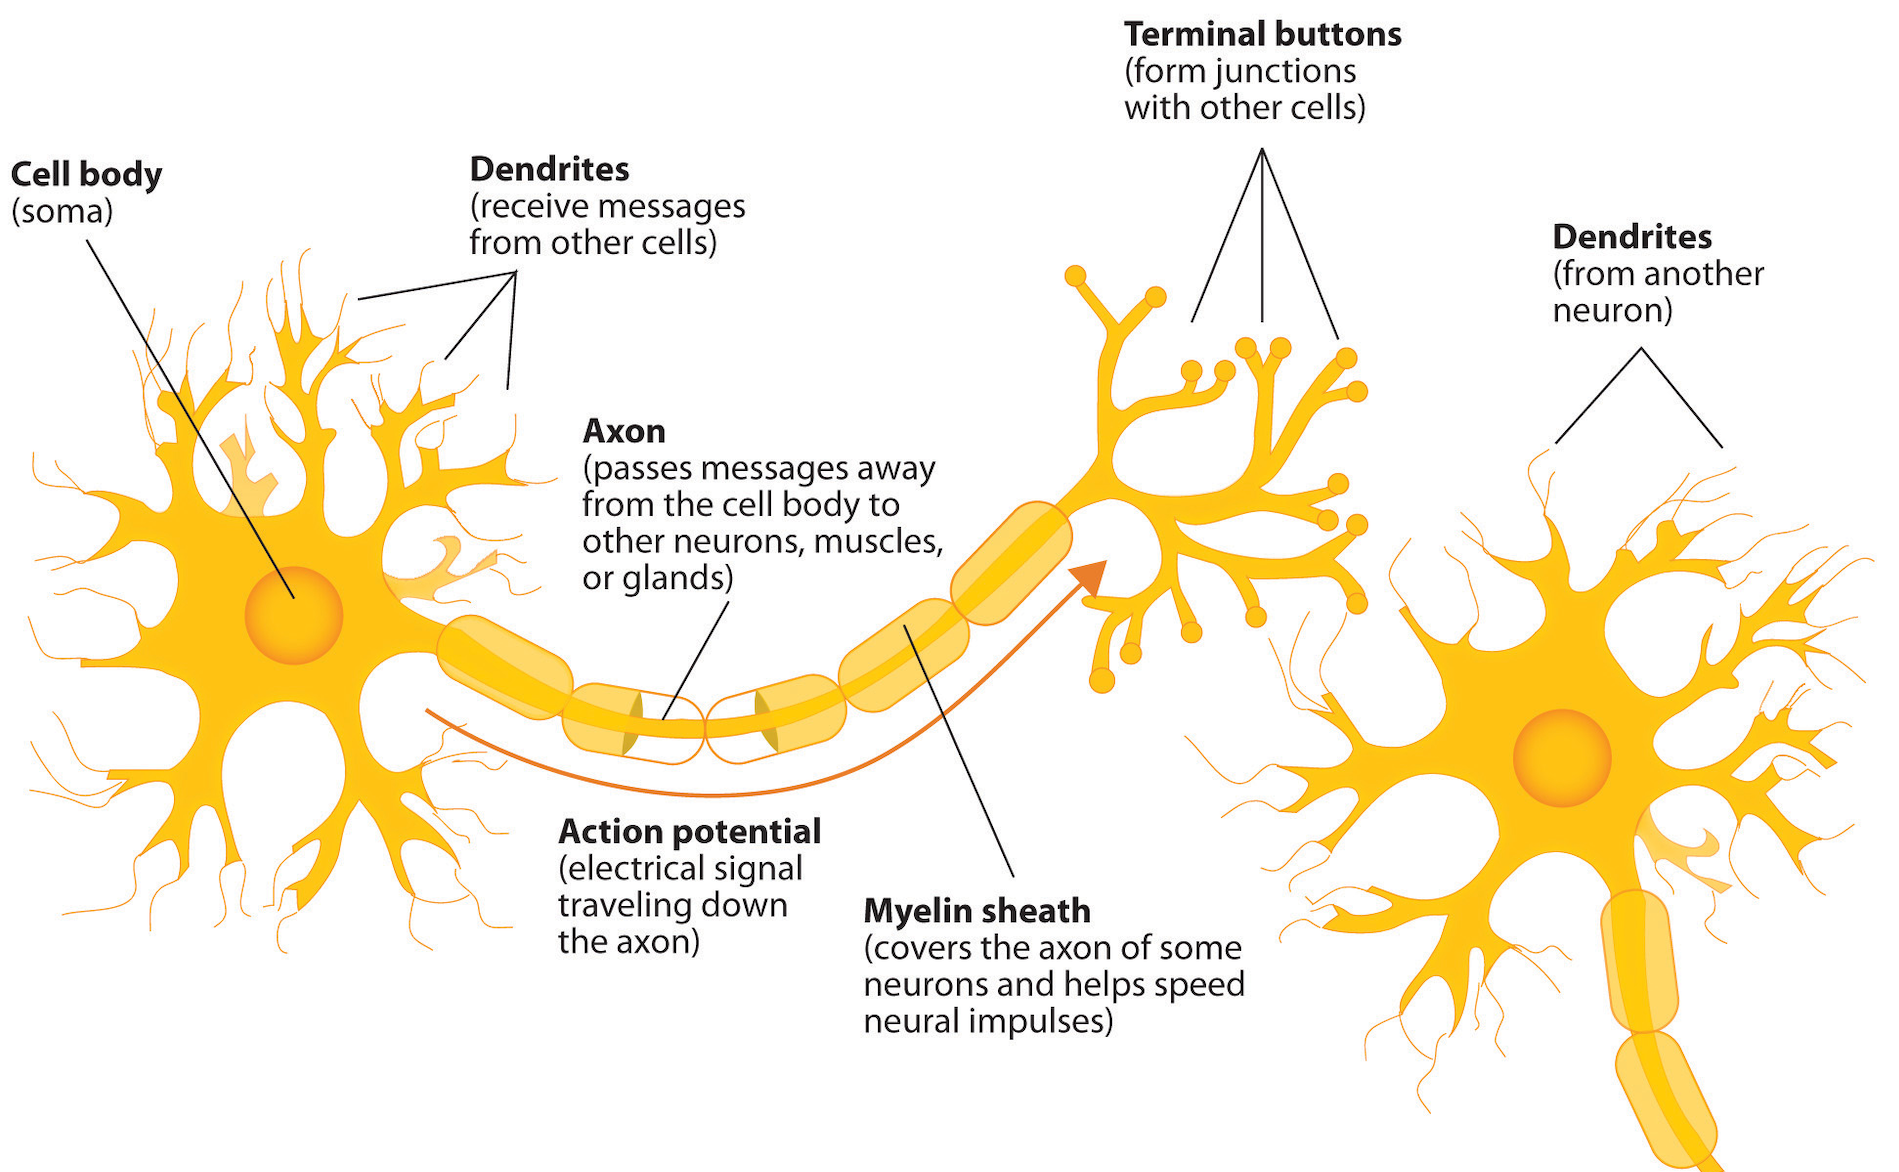
\includegraphics[width = 0.8\textwidth]{../images/components_of_neuron.png}\\[4ex]
\caption{The components of a neuron. Electrical signals are passed down axons and exchanged at terminal boundaries between neurons.}
\label{fig:components_of_neuron}
\end{figure}

In 1943, Warren McCulloch (a neuroscientist) and Walter Pitts (a logician) devised an artificial model of a neuron that is now called a \textdef{McCulloch-Pitts neuron}{McCulloch-Pitts neuron}{an early model of a neuron that aggregates a collection of input binary variables and fires a 1 or 0 based on whether the sum of inputs exceeds some fixed threshold}. A McCulloch-Pitts neuron has a fixed threshold \textvar{b} and takes as input \textvar{n} \textdefnogloss{binary variables} $x_1, \ldots, x_n$, where each of these variables is equal to either 0 or 1. The neuron outputs 1 if $x_1 + \cdots + x_n \geq b$; otherwise, it returns 0. If a McCulloch-Pitts neuron outputs 1, then we say that it \textdefnogloss{fires}. The McCulloch-Pitts neuron with \textvar{n} equal to 2 and \textvar{b} equal to 2 is shown in \autoref{fig:MP_neuron}. The only way that this neuron will fire is if both inputs $x_1$ and $x_2$ are equal to 1.\\

\begin{note}[%
The mathematically astute reader may have noticed that the output of the McCulloch-Pitts neuron in \autoref{fig:MP_neuron} is identical to the logical proposition $(x_1~\texttt{AND}~x_2)$, which explains why these neurons started as a collaboration between a neuroscientist and a logician.
]\end{note}

\begin{figure}[h]
\centering
\mySfFamily
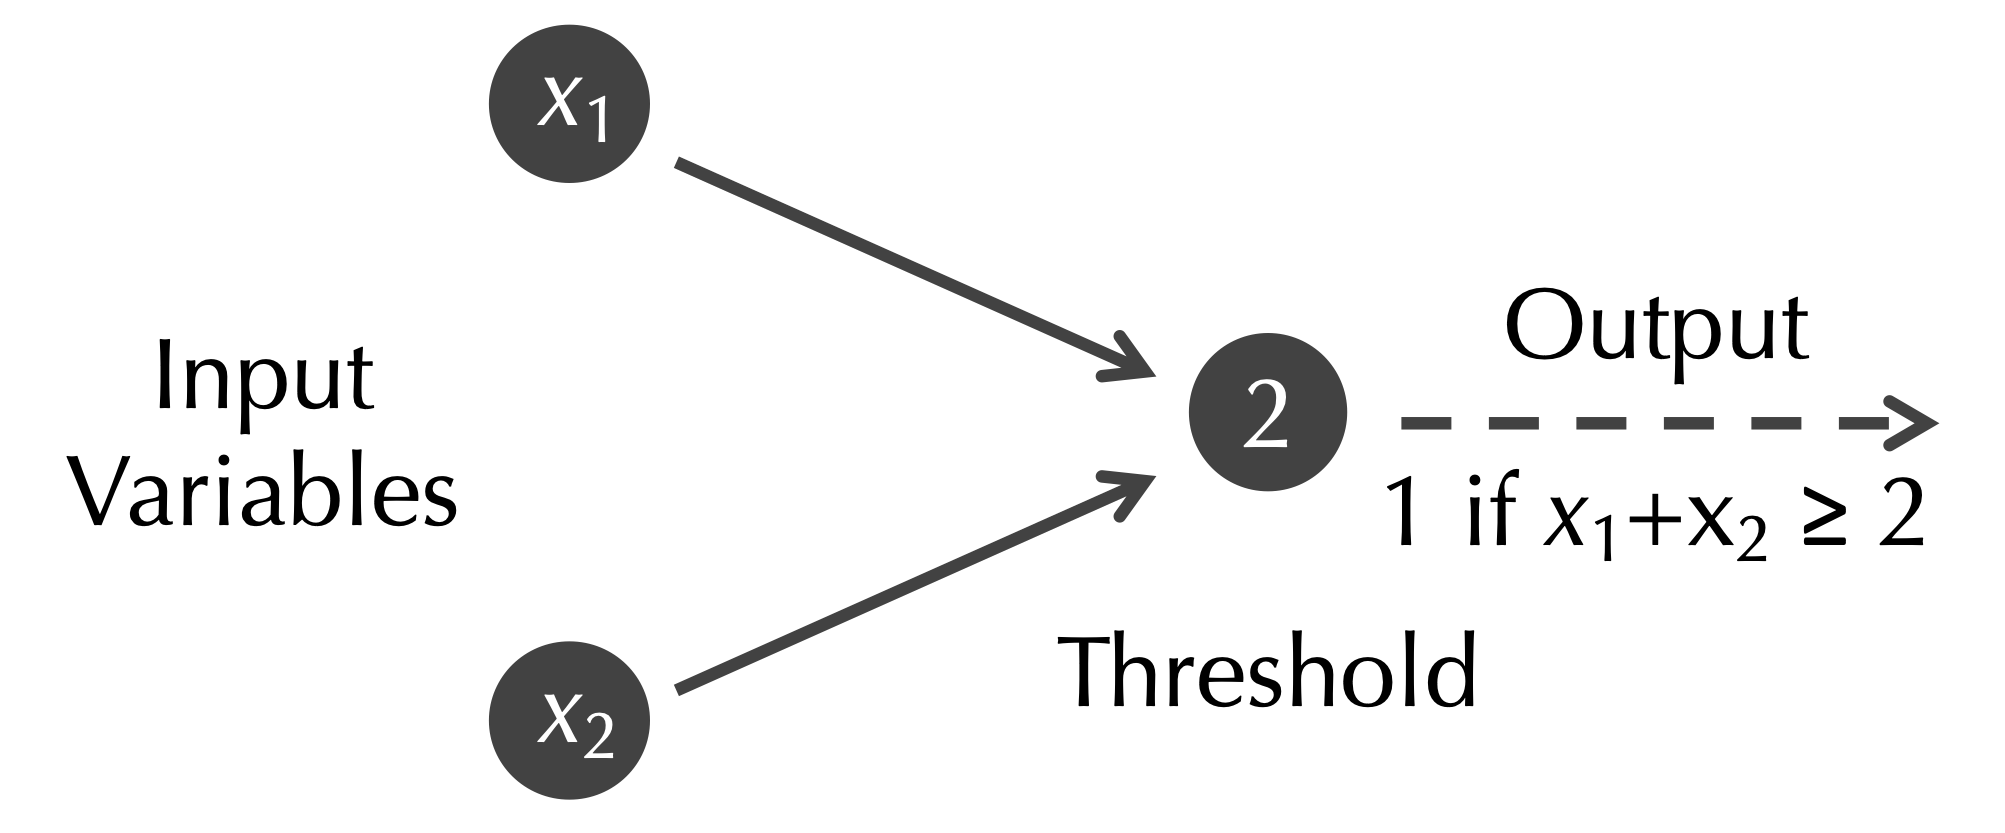
\includegraphics[width = 0.6\textwidth]{../images/MP_neuron.png}
\caption{A McCullough-Pitts neuron with \textvar{n} equal to 2 and \textvar{b} equal to 2. The neuron will fire (i.e., output 1) precisely when both input variables are equal to 1; if either input variable is equal to 0, then $x_1 + x_2$ will be less than \textvar{b} and the neuron will not fire (i.e., it will output 0).}
\label{fig:MP_neuron}
\end{figure}

In 1957, Frank Rosenblatt generalized the McCulloch-Pitts neuron into a \textdef{perceptron}{perceptron}{an artificial neuron that aggregates a weighted average of binary input variables and that outputs 1 if this average is greater than some fixed threshold and 0 otherwise}. A perceptron also has a threshold \textvar{b} and \textvar{n} binary input variables $x_i$, but it includes a collection of constant weights $w_i$, and the neuron fires precisely when the weighted sum $w_1 \cdot x_1 + w_2 \cdot x_2 + \cdots + w_n \cdot x_n$ is at least equal to \textvar{b} (\autoref{fig:perceptron}).\\

\begin{note}[%
A McCulloch-Pitts neuron is a perceptron for which all the $w_i$ are equal to 1.
]\end{note}

\begin{figure}[h]
\centering
\mySfFamily
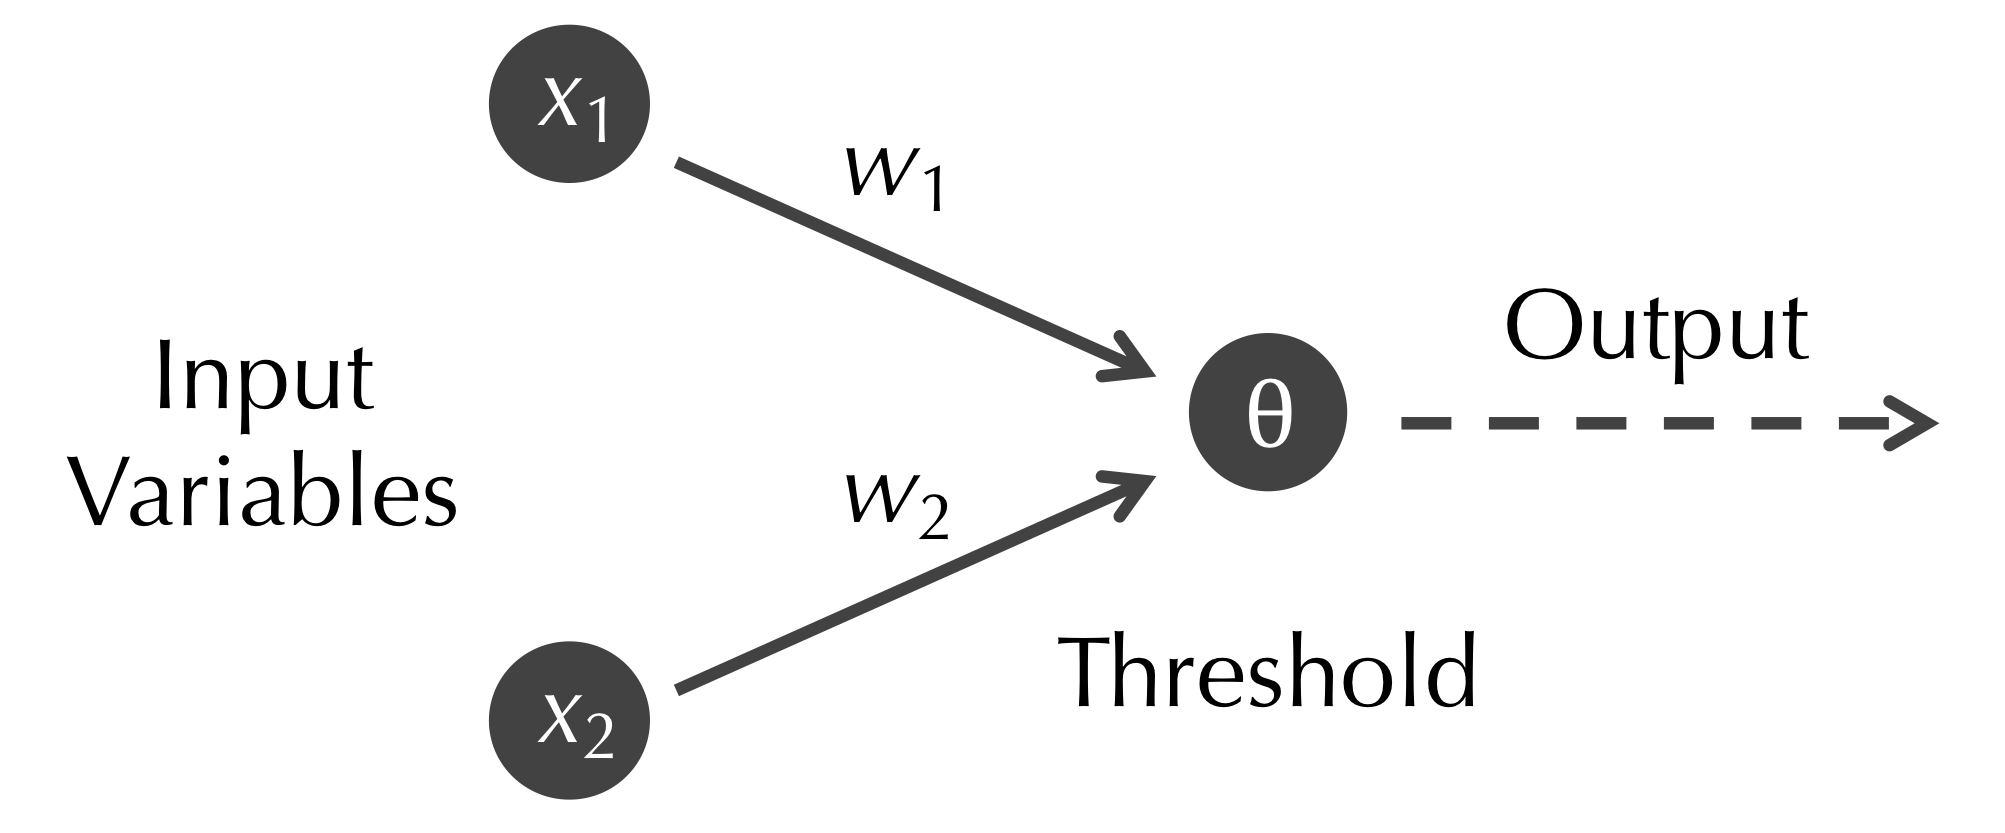
\includegraphics[width = 0.64\textwidth]{../images/perceptron.png}
\caption{A perceptron with two input variables. The perceptron includes a constant threshold and constant weights $\textvar{w}_\text{1}$ and $\textvar{w}_\text{2}$. The perceptron outputs 1 precisely when the weighted sum $\textvar{w}_\text{1} \cdot \textvar{x}_\text{1} + \textvar{w}_\text{2} \cdot \textvar{x}_\text{2}$ is greater than or equal to \textvar{b}, and it outputs 0 otherwise.}
\label{fig:perceptron}
\end{figure}

Modern artificial neurons (\autoref{fig:activation_function}) generalize the perceptron further in two ways. First, the input variables $x_i$ can have arbitrary decimal values (often, these inputs are constrained to be between 0 and 1). Second, rather than the neuron rigidly outputting 1 when $w_1 \cdot x_1 + w_2 \cdot x_2 + \cdots + w_n \cdot x_n$ is greater than or equal to \textvar{b}, we subtract \textvar{b} from the weighted sum and pass the resulting value into a function \textvar{f} called an \textdef{activation function}{activation function}{a function that takes as input a weighted average of input variables in an artificial neuron and whose output is the neuron's output}; that is, the neuron outputs $f(w_1 \cdot x_1 + w_2 \cdot x_2 + \cdots + w_n \cdot x_n - b)$. In this form of the neuron, \textvar{b} is called the \textdefnogloss{bias} of the neuron.

A commonly used activation function is the \textdefnogloss{logistic function}, $f(x) = 1/(1+e^{-x})$, shown in \autoref{fig:logistic_function}. Note that the output of this function ranges between 0 (when its input is very negative) and 1 (when its input is very positive).\\

\begin{figure}[h]
\centering
\mySfFamily
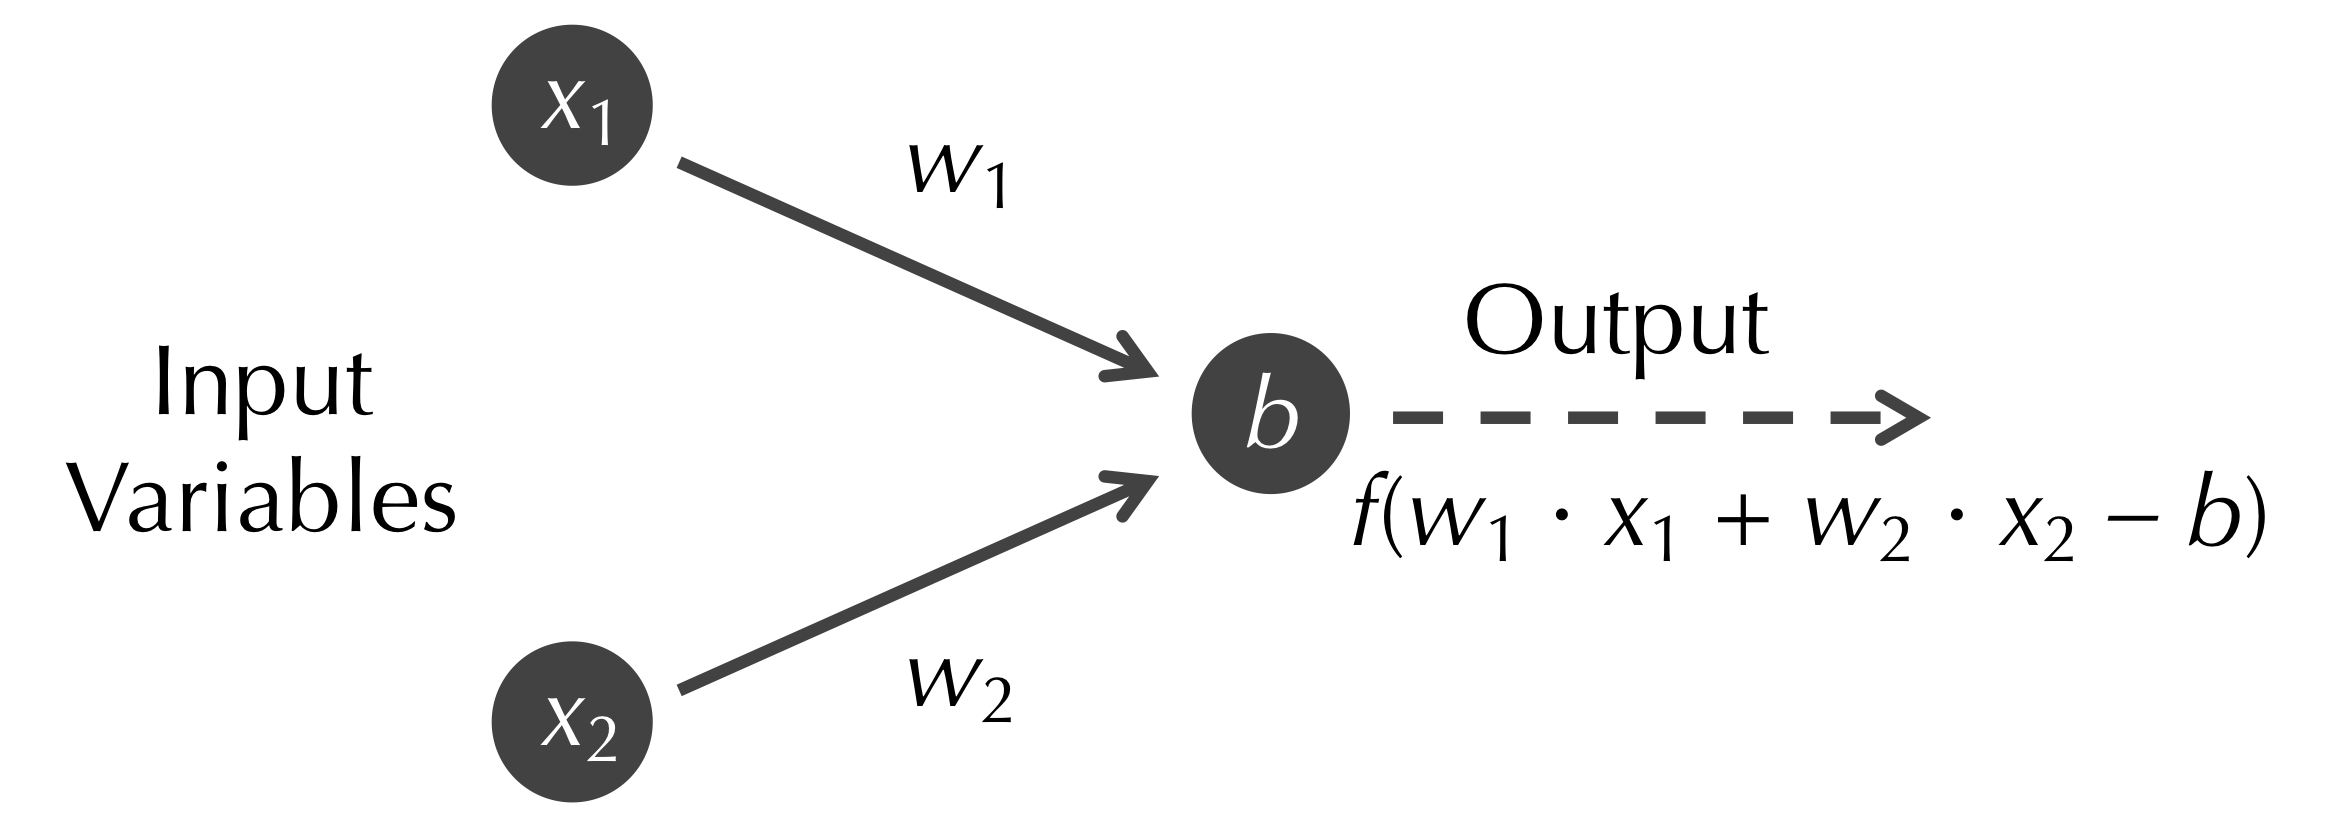
\includegraphics[width = 0.68\textwidth]{../images/activation_function.png}
\caption{A general form of an artificial neuron for two input variables $\textvar{x}_\text{1}$ and $\textvar{x}_\text{2}$, two constant weights $\textvar{w}_\text{1}$ and $\textvar{w}_\text{2}$, a bias \textvar{b}, and an activation function \textvar{f}. The output of the neuron, rather than being strictly 0 or 1, is $\textvar{f}(\textvar{w}_\text{1} \cdot \textvar{x}_\text{1} + \textvar{w}_\text{2} \cdot \textvar{x}_\text{2} - b)$.}
\label{fig:activation_function}
\end{figure}

\begin{figure}[h]
\centering
\mySfFamily
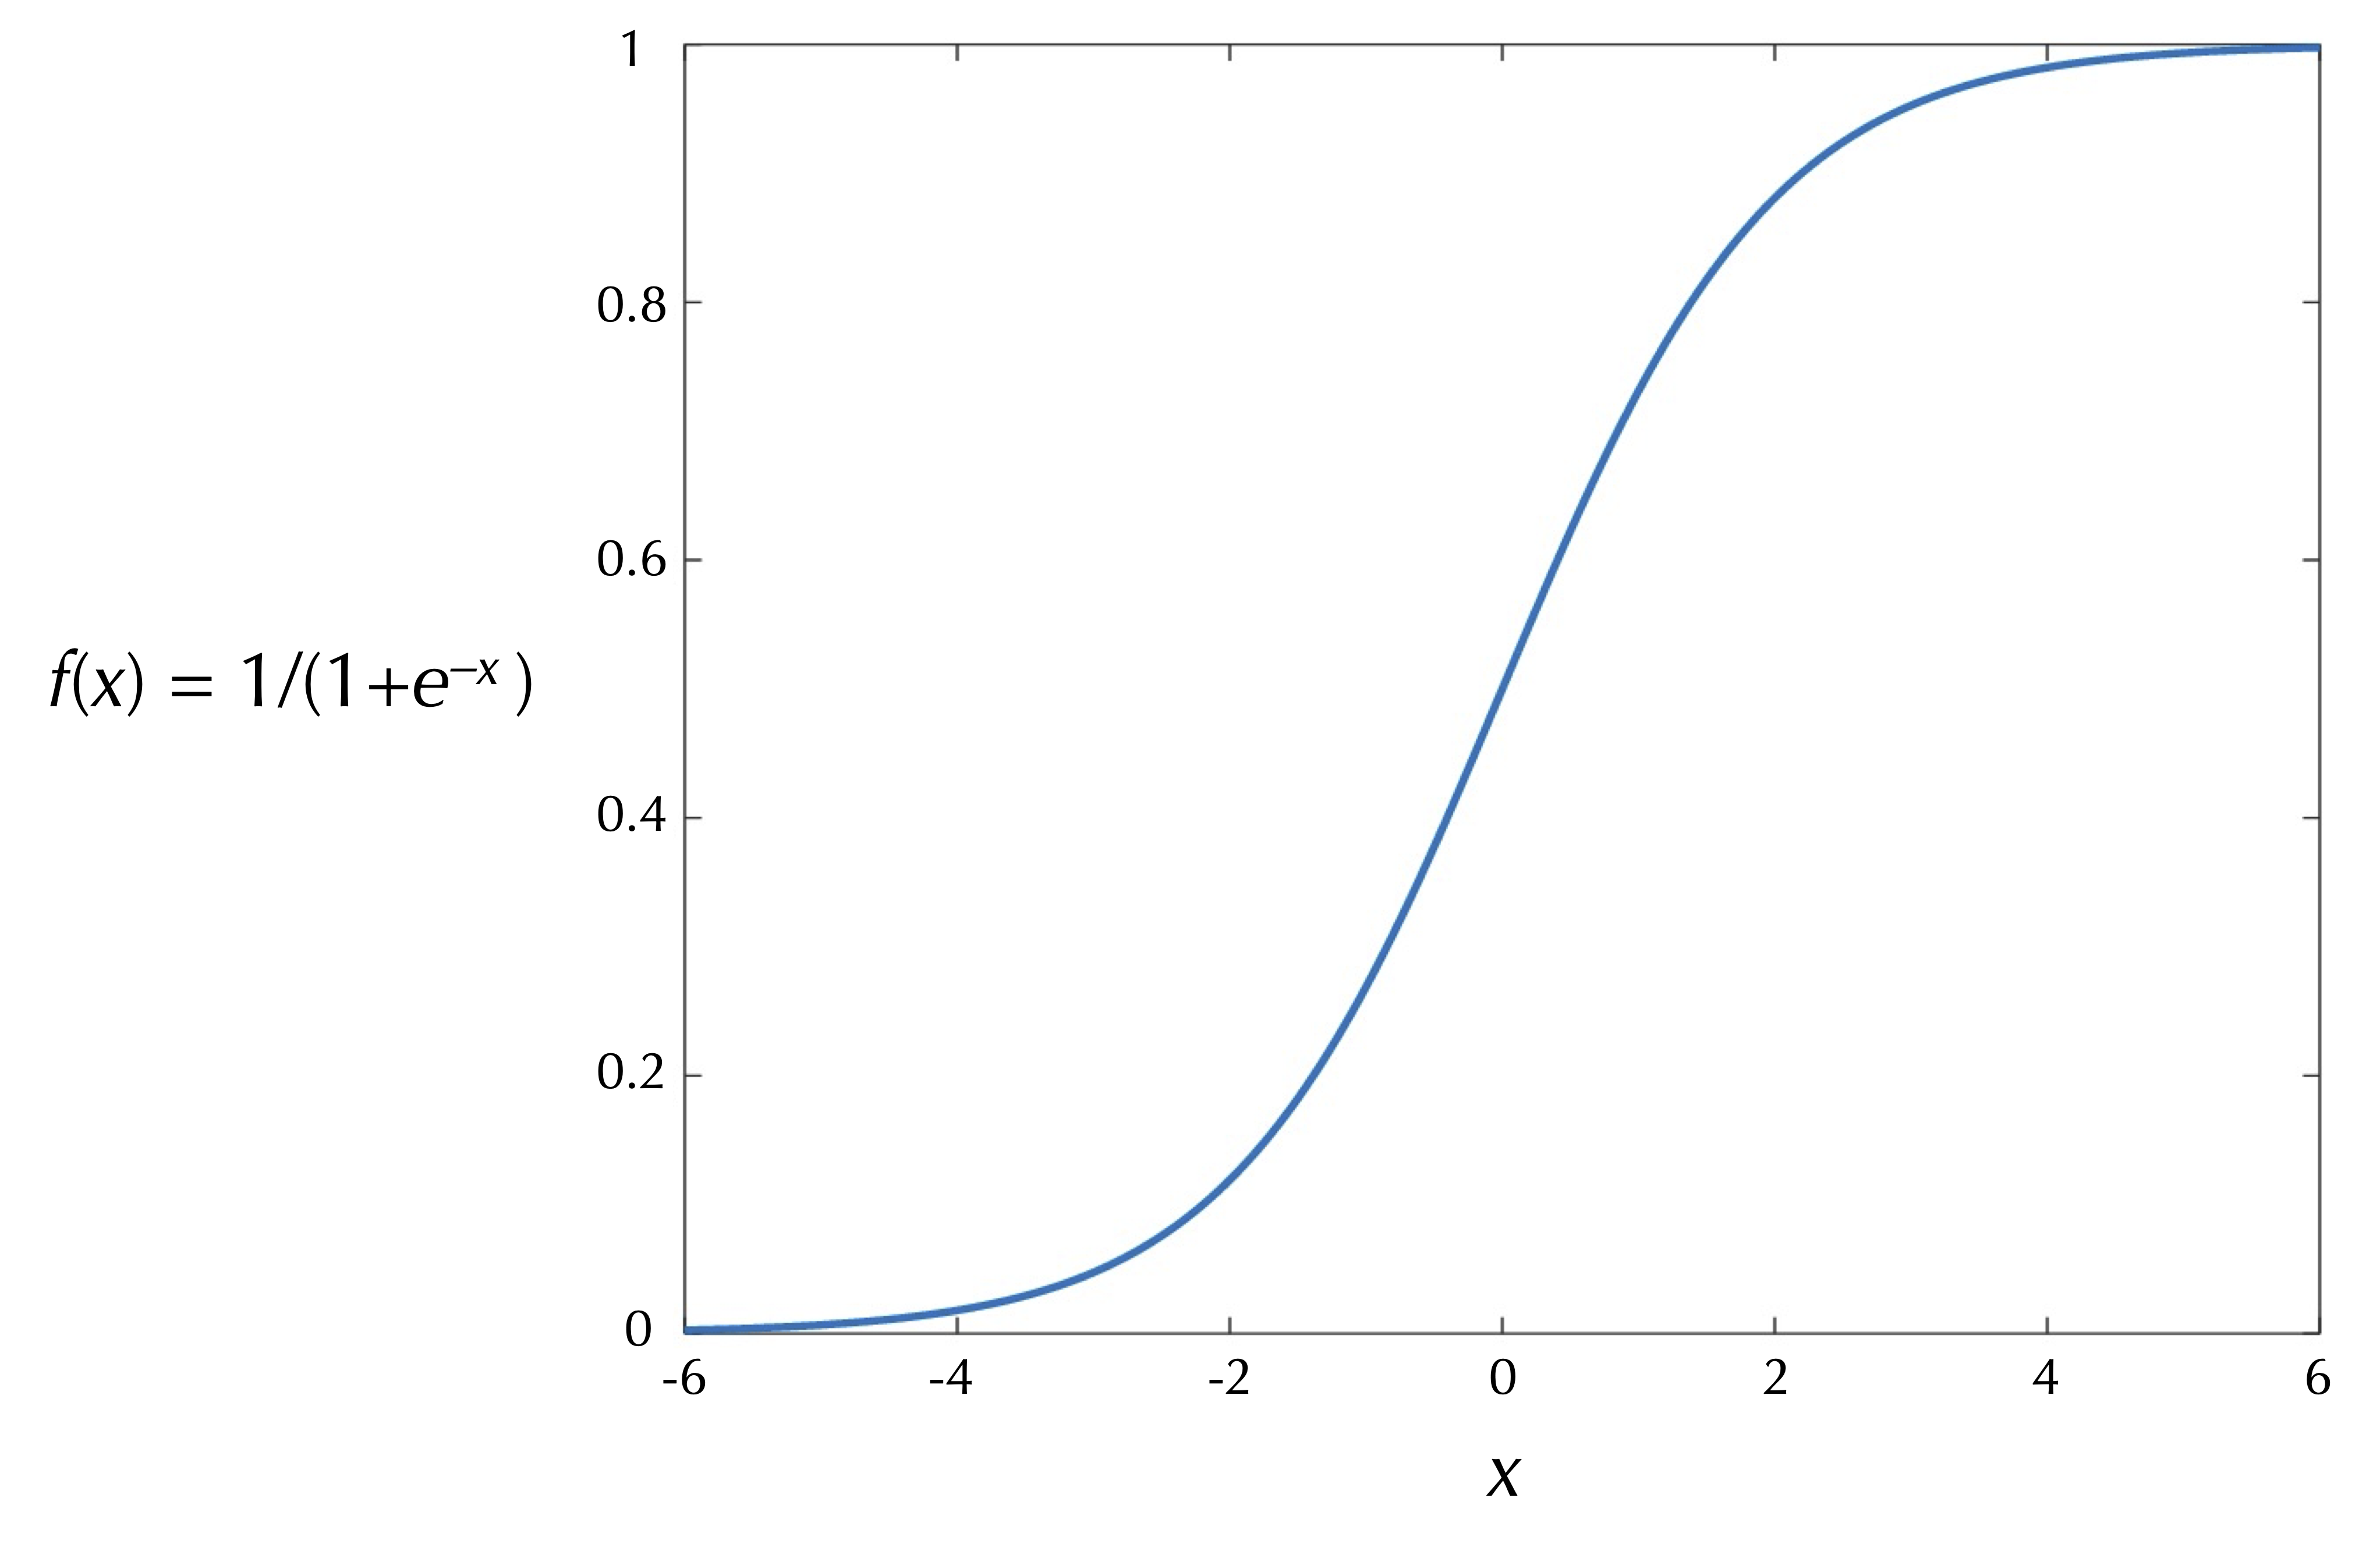
\includegraphics[width = 0.7\textwidth]{../images/logistic_function.png}
\caption{A plot of the logistic function $\textvar{f}(\textvar{x}) = 1/(1+\textvar{e}^{-\textvar{x}})$, an increasing function whose values range between 0 and 1.}
\label{fig:logistic_function}
\end{figure}

\begin{qbox}[%
Because of its simplicity, researchers now often use a ``rectifier'' function: $f(x) = \max(0, x)$. What does the graph of this function look like? What is the activation function used by a perceptron, and how does it differ from the rectifier function?
]\end{qbox}

\phantomsection
\subsection{Framing a classification problem using neural networks}

The outputs of mathematical functions can be used as inputs to other functions via function composition. For example, if $f(x) = 2x-1$, $g(x) = e^x$, and $h(x) = \cos{x}$, then $h(g(f(x))) = \cos{(e^{2x-1})}$. Similarly, we can use artificial neurons as building blocks by linking them together, with the outputs of some neurons serving as inputs to other neurons. Linking artificial neurons together in this way produces a \textdef{neural network}{neural network}{a network of artificial neurons linked together, with the outputs of some neurons used as the input variables for others} such as the one shown in \autoref{fig:neural_network_wbc}, which we will take time to explain.\\

\begin{figure}[h]
\centering
\mySfFamily
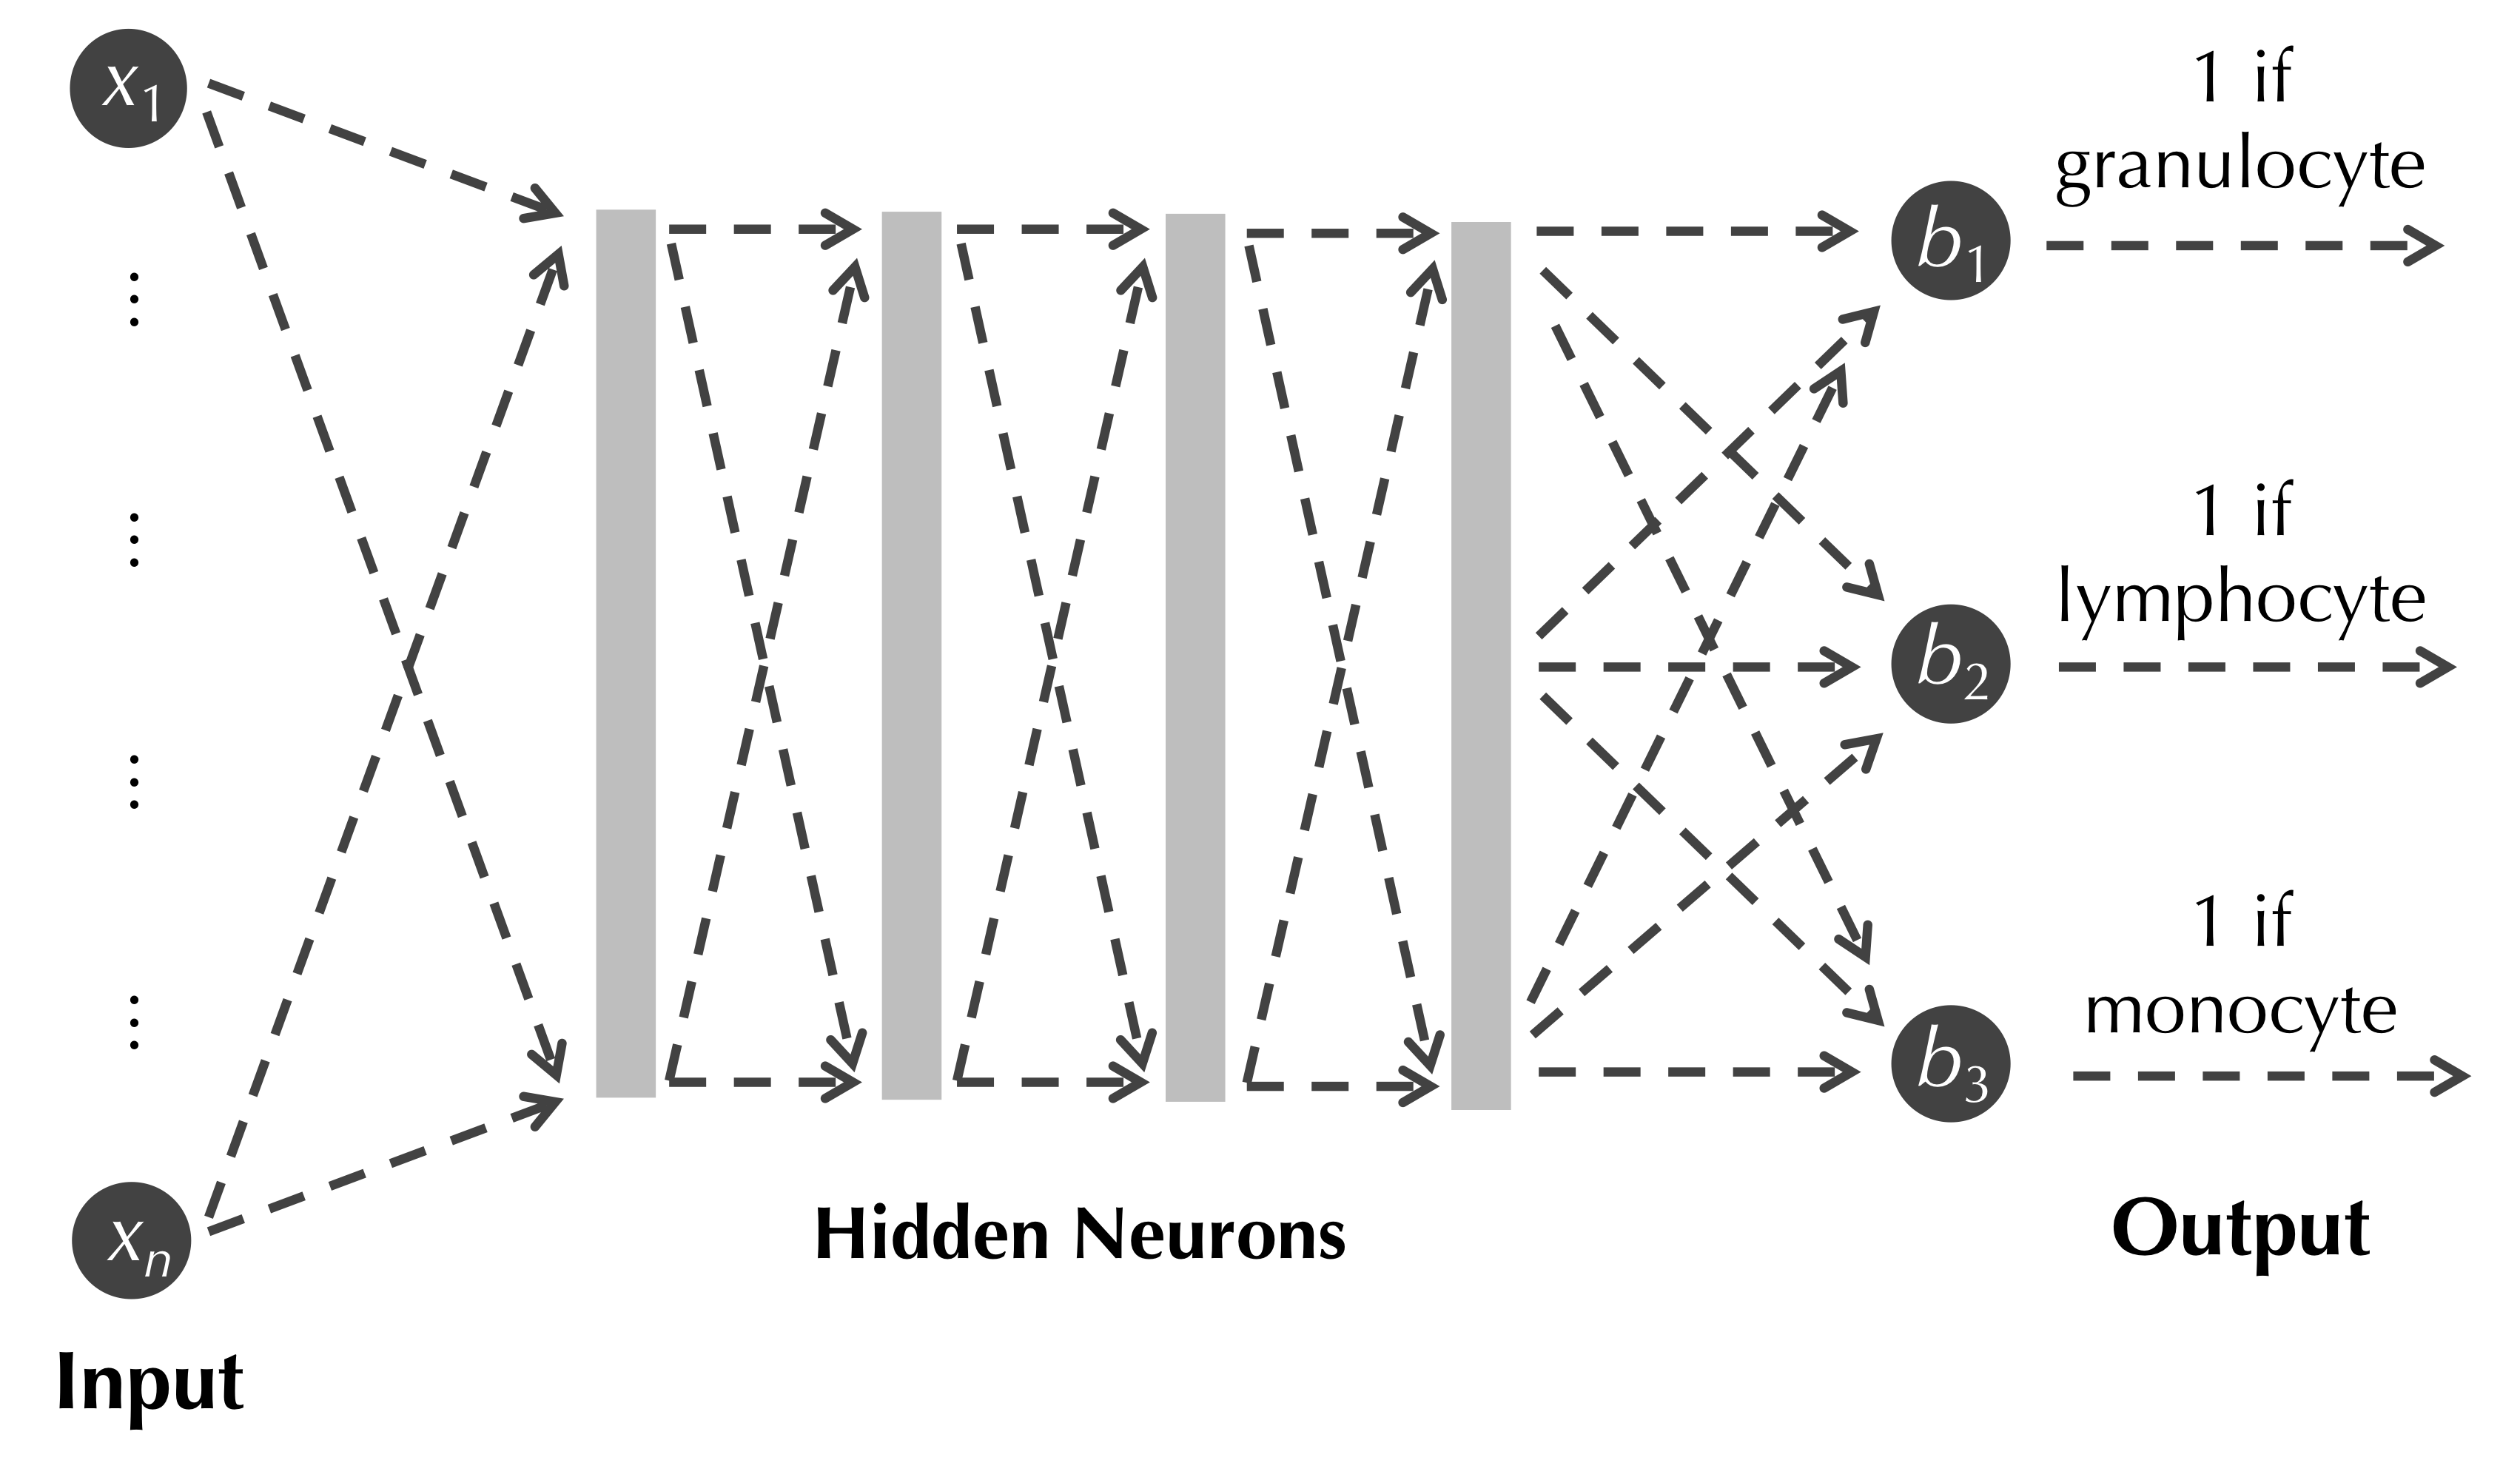
\includegraphics[width = 0.85\textwidth]{../images/neural_network_wbc.png}
\caption{An illustration of a potential neural network used for WBC image classification. This network assumes that each WBC is represented by \textvar{n} features, which serve as the input variables for the network. A number of hidden layers of additional neurons may be used, with connections between some of the neurons in adjacent layers. A final output layer of three neurons corresponds to each of the three WBC classes; our hope is that the weights of the neurons in the network are chosen so that the appropriate neuron outputs a value close to 1 corresponding to an image's class, and that the other two neurons output values close to 0.}
\label{fig:neural_network_wbc}
\end{figure}

We have discussed converting each object \textvar{x} in a dataset (such as our WBC image dataset) into a feature vector $(x_1, x_2, \ldots, x_n)$ representing each of the \textvar{n} feature values of \textvar{x}. In \autoref{fig:neural_network_wbc}, these \textvar{n} variables of the data's feature vectors become the \textvar{n} input variables of the neural network.

We typically then connect all the input variables to most or all of a collection of (possibly many) artificial neurons, called a \textdefnogloss{hidden layer}, which is shown for simplicity as a gray box in \autoref{fig:neural_network_wbc}. If we have \textvar{m} artificial neurons in the hidden layer, and \textvar{n} input variables, then we will have $m$ bias constants as well as $m \cdot n$ weights, one assigned to each edge connecting an input variable to a hidden layer neuron (all these edges are indicated by dashed edges in \autoref{fig:neural_network_wbc}. Our model has quickly accumulated an enormous number of parameters!

The first hidden layer of neurons may then be connected as inputs to neurons in another hidden layer, which are connected to neurons in another layer, and so on. As a result, practical neural networks may have several hidden layers with thousands of neurons, each with their own biases, input weights, and even different activation functions. The most common usage of the term \textdef{deep learning}{deep learning}{an approach that applies neural networks with multiple hidden layers to analyze datasets} refers to solving problems using many hidden layers of neurons; the discussion of the many challenges in designing neural networks for deep learning would cover an entire course much longer than this one.

The remaining question is what the output of our neural network should be. If we would like to apply the network to classify our data into \textvar{k} classes, then we typically will connect the final hidden layer of neurons to \textvar{x} \textdefnogloss{output neurons}. Ideally, if we know that a data point \textvar{x} belongs to the \textvar{i}-th class, then when we use the values of its feature vector as input to the network, we would like for the \textvar{i}-th output neuron to output a value close to 1, and all other output neurons to output a value close to 0. For a neural network to correctly classify objects in our dataset, we must find such an ideal choice for the biases of each neuron and the weights assigned to input variables at each neuron --- assuming that we have decided on which activation function(s) to use for the network's neurons. We will now define quantitatively what makes a given choice of neural network parameters suitable for classification.\\

\begin{qbox}[%
Say that a neural network has 100 input variables, three output neurons, and four hidden layers of 1000 neurons each. Say also that every neuron in one layer is connected as an input to every neuron in the next layer. How many bias parameters will this network have? How many weight parameters will this network have?
]\end{qbox}

\phantomsection
\subsection{Defining the best choice of parameters for a neural network}

We previously introduced cross validation to assess the results of a classification algorithm like k-NN on a collection of data with known classes. To generalize this idea to our neural network classifier, we divide our data that have known classes into a \textdef{training set}{training set}{a subset of a dataset that is used to choose parameters for a model such as a neural network} and a \textdef{test set}{test set}{a subset of a dataset that is used, once parameters have been fixed, to identify the accuracy of a model such as a neural network}, where the training set is typically much larger than the training set. We then seek the choice of parameters for the neural network that ``performs the best'' on the training set, which we will now explain.

Each data point \textvar{x} in the training set has a ground truth classification vector $\mathbf{c}(x) = (c_1, c_2, \ldots, c_k)$, where if \textvar{x} belongs to class \textvar{j}, then $c_j$ is equal to 1, and the other elements of $\mathbf{c}(x)$ are equal to 0. The point \textvar{x} also has an output vector $\mathbf{o}(x) = (o_1, o_2, \ldots, o_k)$, where for each \textvar{i}, $o_i$  is the output of the \textvar{i}-th output vector in the network when \textvar{x} is used as the network's input. The neural network is doing well at identifying the class of \textvar{x} when the classification vector $\mathbf{c}(x)$ is similar to the output vector $\mathbf{o}(x)$.

Fortunately, we have been using a method of comparing two vectors throughout this book. The RMSD between an object's classification vector and its output vector for a given neural network measures how well the network classified this data point, with a value close to 0 representing a good fit. We can obtain a good measure of how well a neural network with given weight and bias parameters performs on a training set on the whole by taking the average RMSD between classification and output vectors over every element in the training set. We therefore would like to choose the biases and input weights for the neural network that minimize this average RMSD for all objects in the training set.

Once we have chosen a collection of bias and weight parameters for our network that perform well on the training set, we then assess how well these parameters performs on the test set. To this end, we can insert the feature vector of each test set object \textit{x} as input into the network, and then consult the output vector $\mathbf{o}(x) = (o_1, o_2, \ldots, o_k)$ for this object. Whichever \textvar{i} maximizes $o_i$ for this output vector becomes the assigned class of \textvar{x}. We can then use metrics for quantifying the quality of a classifier such as accuracy, recall, specificity, and precision, to determine how well the neural network is performing at classifying objects from the test set.

This discussion has assumed that we can easily determine the best choice of network parameters to produce a low mean RMSD for the training set. But how can we find this set of parameters in the first place?

\phantomsection
\subsection{Exploring a parameter space}

The typical neural network contains anywhere from thousands to billions of biases and input weights. We can think of these weight parameters as forming the coordinates of a long vector in a high-dimensional space. From the perspective of producing low mean RMSD between output and classification vectors over a collection of training data, the vast majority of the points in this space (i.e., choices of network parameters) are worthless. In this vast landscape, a tiny number of these parameter choices will provide a good result on our training set, and even with substantial computational resources, finding one of these points is daunting.

The situation in which we find ourselves is remarkably similar to that of a bacterium exploring an environment with sparse food resources, or identifying the conformation of a protein having the lowest potential energy. Borrowing this idea, we would like to apply a \textit{local search} algorithm to explore the parameter space.

As with \textit{ab initio} structure prediction, we could start with a random choice of parameters, make a variety of small changes to the parameter values to obtain ``nearby'' parameter vectors, and then update our current parameters to the choice of nearby parameters that produce the greatest decrease in mean RMSD between output and classification vectors. We continue this process of making small parameter changes until this mean RMSD stops decreasing. This local search algorithm powers the most popular approach for determining parameters for a neural network, called \textdefnogloss{gradient descent}.\\

\begin{qbox}[%
What does a local minimum mean in the context of parameter search?
]\end{qbox}

Just as we run \textit{ab initio} structure prediction algorithms using many different initial protein conformations, to avoid getting stuck in a \textit{local minimum}, we run gradient descent for many different sets of randomly chosen initial parameters. In the end, we take the choice of parameters minimizing mean RMSD over all the runs of gradient descent.

\phantomsection
\subsection{The curse of dimensionality, Alphafold, and final reflections}

AT SOME POINT, CALL BACK TO ALPHAFOLD. Critical idea here is that a neural network can be thought of a big, bulky thing that takes some things and produces others, a complicated function. We already know how to vectorize structures, so we could train a neural network to take sequences (encoded as vectors) and produce their shape vectors. What AlphaFold does is more complicated than this, involving a few different neural networks, but the idea is still the same.

Even though neural networks have had successes, they are not a cure-all, and there are still many problems in which they are struggling to make in-roads. We have encountered many themes in this work, from emergent behavior from simple rules, to the power of randomness to solve practical problems, to how to explore a large, sparsely populated space, but we hope that above all, this is the largest one. Despite what we have had the time and space to present here, many aspects of biology and its intersection with computation still remain like a bacterium's world: an untouched universe waiting to be explored.

%MOVE THIS DOWN
%However, because the neural network has many bias and weight parameters, we should be wary of the curse of dimensionality. It may be difficult to obtain a network and parameters that perform well on the training set, and even if a model has a low mean RMSD for the training set, it may perform horribly on the test set. (The former situation is called ``underfitting'' and the latter is called ``overfitting''.)

%Neural networks aren't a cure all and they come with their own issues.

% Something about the number of parameters in the AlphaFold network (21 million). Energy usage?
%
%We have a huge amount of freedom when building neural networks, since we can link up neurons however we like, and since the weights of all incoming edges at each neuron are allowed to vary, as well as the activation function used at each neuron. This freedom will mean that the number of possible neural networks is incomprehensibly large, so that neural networks are very powerful, but they can also be difficult to interpret.



\FloatBarrier

\newpage
\phantomsection
\section{Exercises}

\phantomsection
\subsection{Neural networks and logical connectives}

One of the strengths of artificial neurons and neural networks is that it can be shown that their output can mimic, at least approximately, any function. In the case of classification, this means that if some function $g(x_1, \ldots x_n)$ exists that does a good job of classifying data with \textvar{n} features, then some neural network exists that will replicate this function: we just need to find the right set of network parameters.

We say that a neural network with input variables $x_1, \ldots x_n$ \textdefnogloss{represents} a function $g(x_1, \ldots, x_n)$ if for any choice of input variables $x_1$, the output of the neural network is equal to $g(x_1, \ldots, x_n)$. We provide two exercises providing some practice on finding neural networks that represent relatively simple functions.\\

\begin{exercise}[%
Consider the function $g(x_1, x_2)$ for binary input variables $x_1$ and $x_2$ that outputs 0 only when $x_1$ and $x_2$ are both equal to 1 and that outputs 1 for other choices of $x_1$ and $x_2$. (The function \textvar{g} is known as a ``\texttt{NAND} gate'').  Find a single perceptron that represents \textvar{g}. 
]\end{exercise}

\begin{exercise}[%
Consider the function $g(x_1, x_2)$ for binary input variables $x_1$ and $x_2$ that outputs 1 when $x_1 \neq x_2$ and 0 when $x_1 = x_2$. (The function \textvar{g} is known as an ``\texttt{XOR} gate'').  It can be shown that no single perceptron represents \textvar{g}; find a neural network of perceptrons that represents \textvar{g}.
]\end{exercise}

\phantomsection
\subsection{A little fun with lost cities}

\begin{exercise}[%
Consider the three points $x = (-8, 1)$, $y = (7, 6)$, and $z = (10, -2)$. Say that the distances from these points to some point \textvar{w} with unknown location are as follows: $d(x, w) = 13$; $d(y, w) = 3$; $d(z, w) = 10$. Where is \textvar{w}?
]\end{exercise}

\phantomsection
\subsection{More on the curse of dimensionality}

Intuitively, having a large number of features in our data (i.e., a large dimension of \textvar{n} in our feature vector) is a good thing. Yet consider \autoref{fig:curse_of_dimensionality_two_irises}, which plots the petal width and length of two iris flowers. It would be a horrible idea to extrapolate anything from the line connecting these two points, as it indicates that these two variables are inversely coordinated, the \textit{opposite} of the true correlation that we found in \autoref{fig:iris_flowers_regression_line}.

This example provides another reason why we reduce the dimension of a dataset when the number of objects in our dataset is smaller than the number of features of each object. Furthermore, when fitting a \textvar{d}-dimensional hyperplane to a collection of data, we need to be careful with selecting too large of a value of \textvar{d}, especially if we do not have many data points. \\

\begin{figure}[h]
\centering
\mySfFamily
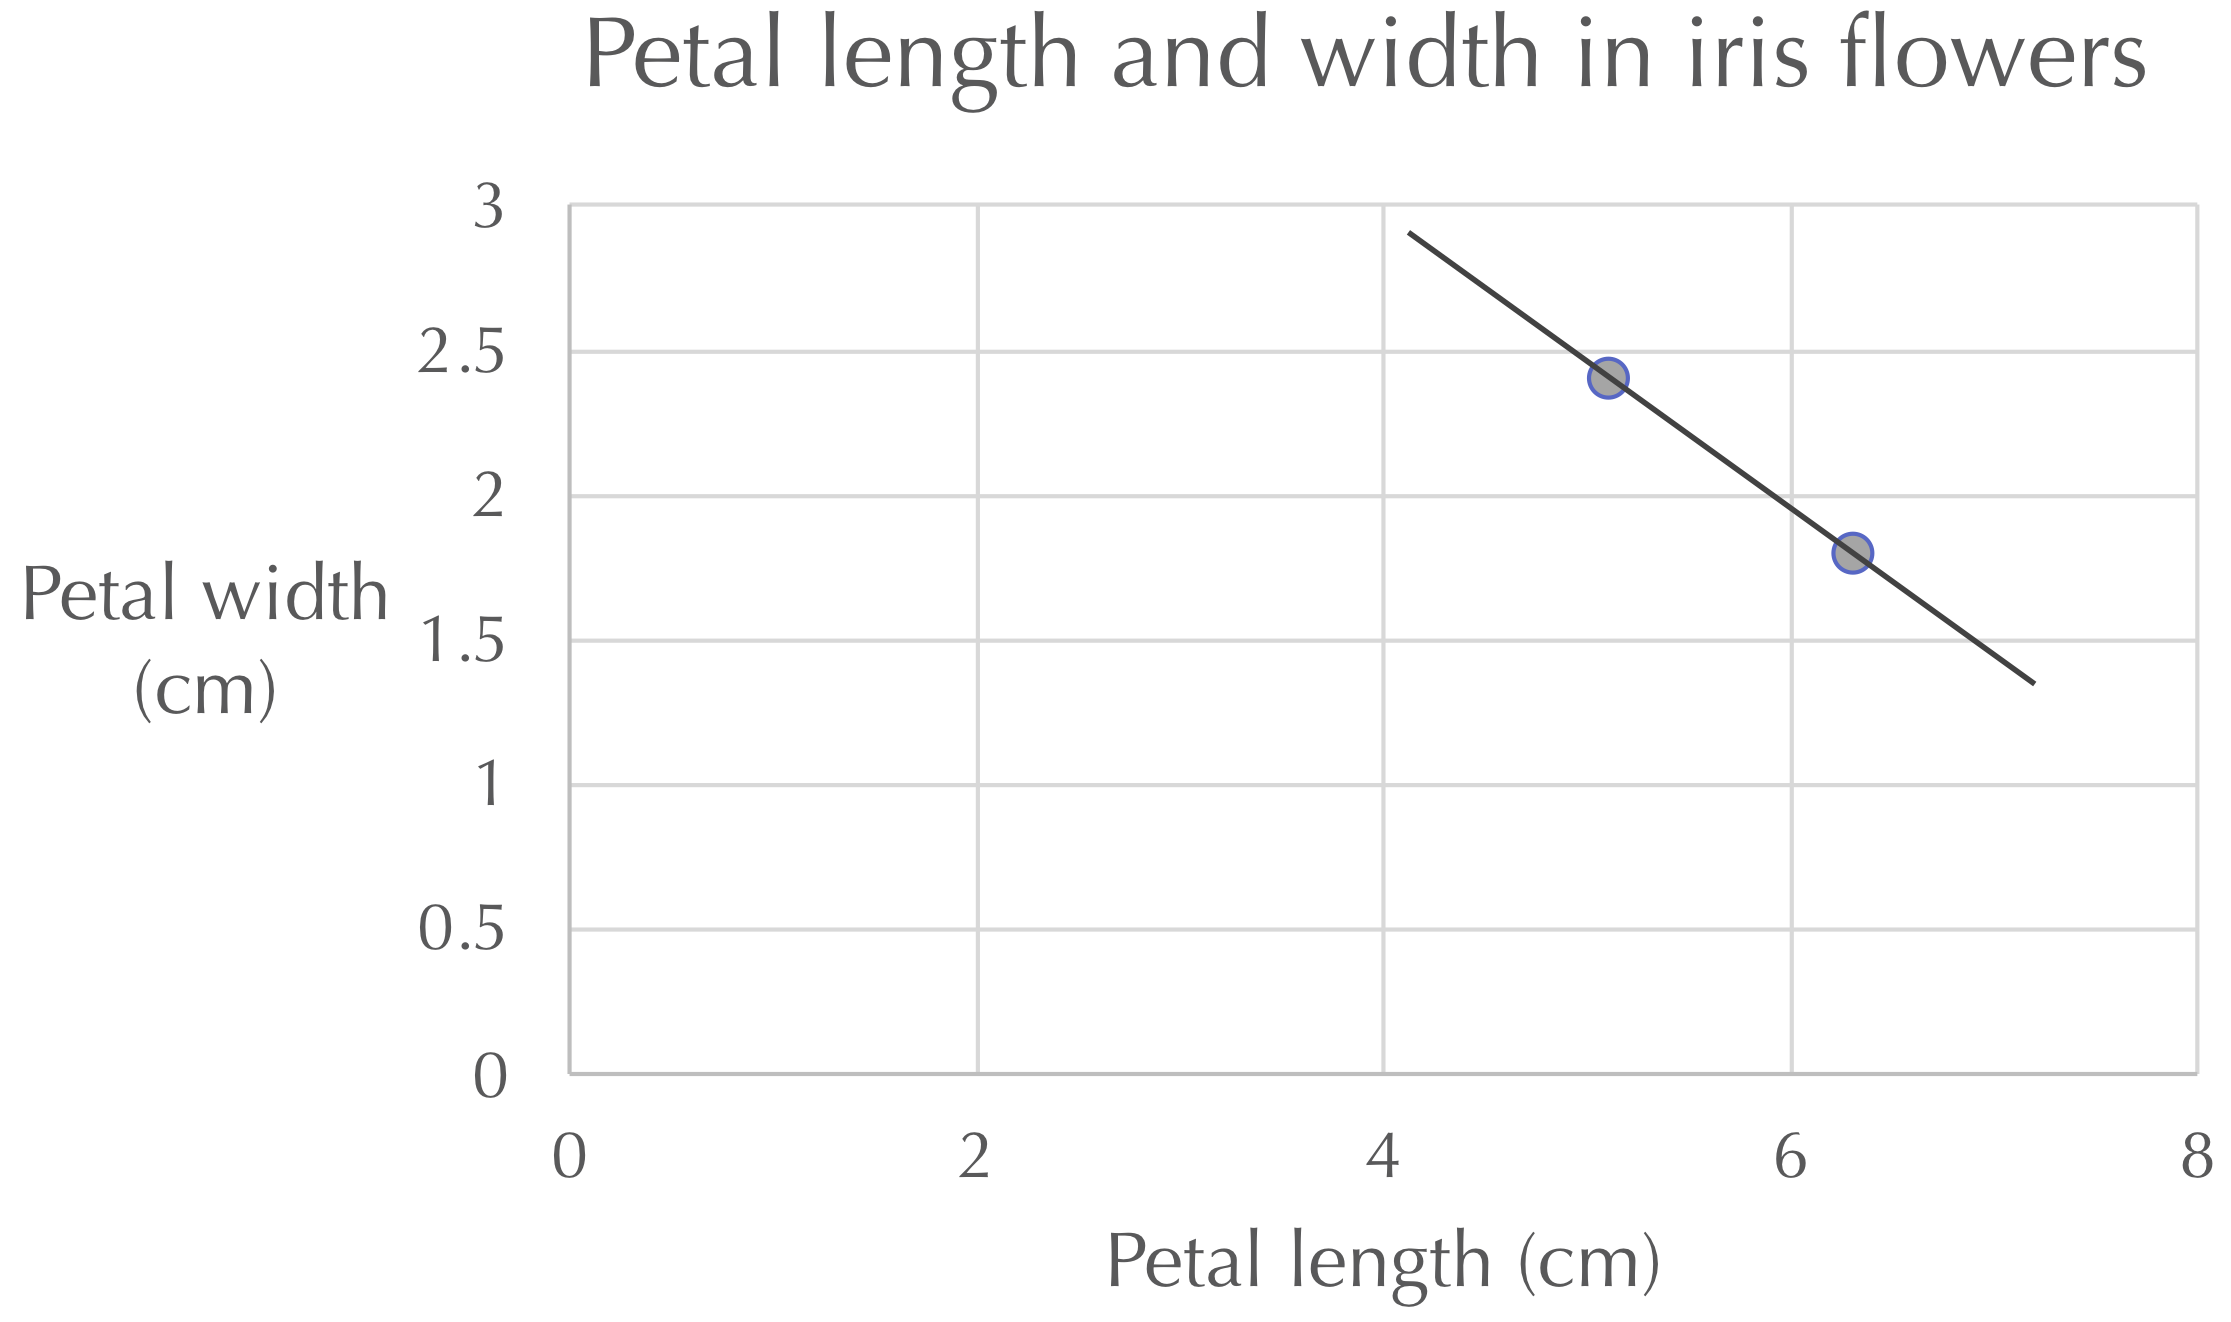
\includegraphics[width = 0.7\textwidth]{../images/curse_of_dimensionality_two_irises.png}
\caption{Petal length plotted against petal width for two flowers in the iris flower dataset. Because of random chance and small sample size, these two flowers demonstrate an inverse correlation between petal length and width, the opposite of the true correlation found in \autoref{fig:iris_flowers_regression_line}.}
\label{fig:curse_of_dimensionality_two_irises}
\end{figure}

\begin{exercise}[%
What is the minimum number of points in three-dimensional space such that we cannot guarantee that there is a plane containing them all? Provide a conjecture as to the minimum number of points in \textvar{n}-dimensional space such that we cannot guarantee that there is a \textvar{d}-dimensional hyperplane containing them all.
]\end{exercise}

\phantomsection
\subsection{Irises and feature selection}

\fudgespace

\begin{exercise}[%
The iris flower dataset has four features. Apply PCA with $d = 2$ to reduce the dimension of this dataset. Then, apply k-NN with \textvar{k} equal to 1 and cross validation with \textvar{f} equal to 10 to the resulting vectors of reduced dimension to obtain a confusion matrix. What are the accuracy, recall, specificity, and precision? How do they compare against the results of using all four iris features from \autoref{fig:iris_confusion_matrix}?
]\end{exercise}

\begin{exercise}[%
Another way to reduce the dimension of a dataset is to eliminate features from the dataset. Apply k-NN with \textvar{k} equal to 1 and cross validation with \textvar{f} equal to 10 to the iris flower dataset using only the two features petal width and petal length. Then, run the same classifier on your own choice of two iris features to obtain a confusion matrix. How do the results compare against the result of the previous exercise (which used PCA instead of feature elimination) and \autoref{fig:iris_confusion_matrix} (which used all four features)?
]\end{exercise}

%\phantomsection
%\subsection{More classification of our WBC image dataset}
%
%\begin{exercise}[%
%Add nuclear size to dataset -- call back to the main text when we mentioned this. In main text, say that we explore as an exercise?
%]\end{exercise}
%
%\begin{exercise}[%
%Yanjing's other exercise here.
%]\end{exercise}
%
%\begin{exercise}[%
%Neural network exercise on WBC image dataset.
%]\end{exercise}

